% Options for packages loaded elsewhere
\PassOptionsToPackage{unicode}{hyperref}
\PassOptionsToPackage{hyphens}{url}
%
\documentclass[
]{article}
\usepackage{amsmath,amssymb}
\usepackage{lmodern}
\usepackage{iftex}
\ifPDFTeX
  \usepackage[T1]{fontenc}
  \usepackage[utf8]{inputenc}
  \usepackage{textcomp} % provide euro and other symbols
\else % if luatex or xetex
  \usepackage{unicode-math}
  \defaultfontfeatures{Scale=MatchLowercase}
  \defaultfontfeatures[\rmfamily]{Ligatures=TeX,Scale=1}
\fi
% Use upquote if available, for straight quotes in verbatim environments
\IfFileExists{upquote.sty}{\usepackage{upquote}}{}
\IfFileExists{microtype.sty}{% use microtype if available
  \usepackage[]{microtype}
  \UseMicrotypeSet[protrusion]{basicmath} % disable protrusion for tt fonts
}{}
\makeatletter
\@ifundefined{KOMAClassName}{% if non-KOMA class
  \IfFileExists{parskip.sty}{%
    \usepackage{parskip}
  }{% else
    \setlength{\parindent}{0pt}
    \setlength{\parskip}{6pt plus 2pt minus 1pt}}
}{% if KOMA class
  \KOMAoptions{parskip=half}}
\makeatother
\usepackage{xcolor}
\usepackage[margin=1in]{geometry}
\usepackage{longtable,booktabs,array}
\usepackage{calc} % for calculating minipage widths
% Correct order of tables after \paragraph or \subparagraph
\usepackage{etoolbox}
\makeatletter
\patchcmd\longtable{\par}{\if@noskipsec\mbox{}\fi\par}{}{}
\makeatother
% Allow footnotes in longtable head/foot
\IfFileExists{footnotehyper.sty}{\usepackage{footnotehyper}}{\usepackage{footnote}}
\makesavenoteenv{longtable}
\usepackage{graphicx}
\makeatletter
\def\maxwidth{\ifdim\Gin@nat@width>\linewidth\linewidth\else\Gin@nat@width\fi}
\def\maxheight{\ifdim\Gin@nat@height>\textheight\textheight\else\Gin@nat@height\fi}
\makeatother
% Scale images if necessary, so that they will not overflow the page
% margins by default, and it is still possible to overwrite the defaults
% using explicit options in \includegraphics[width, height, ...]{}
\setkeys{Gin}{width=\maxwidth,height=\maxheight,keepaspectratio}
% Set default figure placement to htbp
\makeatletter
\def\fps@figure{htbp}
\makeatother
\setlength{\emergencystretch}{3em} % prevent overfull lines
\providecommand{\tightlist}{%
  \setlength{\itemsep}{0pt}\setlength{\parskip}{0pt}}
\setcounter{secnumdepth}{-\maxdimen} % remove section numbering
\usepackage{xcolor}
\definecolor{aliceblue}{HTML}{F0F8FF}
\definecolor{antiquewhite}{HTML}{FAEBD7}
\definecolor{aqua}{HTML}{00FFFF}
\definecolor{aquamarine}{HTML}{7FFFD4}
\definecolor{azure}{HTML}{F0FFFF}
\definecolor{beige}{HTML}{F5F5DC}
\definecolor{bisque}{HTML}{FFE4C4}
\definecolor{black}{HTML}{000000}
\definecolor{blanchedalmond}{HTML}{FFEBCD}
\definecolor{blue}{HTML}{0000FF}
\definecolor{blueviolet}{HTML}{8A2BE2}
\definecolor{brown}{HTML}{A52A2A}
\definecolor{burlywood}{HTML}{DEB887}
\definecolor{cadetblue}{HTML}{5F9EA0}
\definecolor{chartreuse}{HTML}{7FFF00}
\definecolor{chocolate}{HTML}{D2691E}
\definecolor{coral}{HTML}{FF7F50}
\definecolor{cornflowerblue}{HTML}{6495ED}
\definecolor{cornsilk}{HTML}{FFF8DC}
\definecolor{crimson}{HTML}{DC143C}
\definecolor{cyan}{HTML}{00FFFF}
\definecolor{darkblue}{HTML}{00008B}
\definecolor{darkcyan}{HTML}{008B8B}
\definecolor{darkgoldenrod}{HTML}{B8860B}
\definecolor{darkgray}{HTML}{A9A9A9}
\definecolor{darkgreen}{HTML}{006400}
\definecolor{darkgrey}{HTML}{A9A9A9}
\definecolor{darkkhaki}{HTML}{BDB76B}
\definecolor{darkmagenta}{HTML}{8B008B}
\definecolor{darkolivegreen}{HTML}{556B2F}
\definecolor{darkorange}{HTML}{FF8C00}
\definecolor{darkorchid}{HTML}{9932CC}
\definecolor{darkred}{HTML}{8B0000}
\definecolor{darksalmon}{HTML}{E9967A}
\definecolor{darkseagreen}{HTML}{8FBC8F}
\definecolor{darkslateblue}{HTML}{483D8B}
\definecolor{darkslategray}{HTML}{2F4F4F}
\definecolor{darkslategrey}{HTML}{2F4F4F}
\definecolor{darkturquoise}{HTML}{00CED1}
\definecolor{darkviolet}{HTML}{9400D3}
\definecolor{deeppink}{HTML}{FF1493}
\definecolor{deepskyblue}{HTML}{00BFFF}
\definecolor{dimgray}{HTML}{696969}
\definecolor{dimgrey}{HTML}{696969}
\definecolor{dodgerblue}{HTML}{1E90FF}
\definecolor{firebrick}{HTML}{B22222}
\definecolor{floralwhite}{HTML}{FFFAF0}
\definecolor{forestgreen}{HTML}{228B22}
\definecolor{fuchsia}{HTML}{FF00FF}
\definecolor{gainsboro}{HTML}{DCDCDC}
\definecolor{ghostwhite}{HTML}{F8F8FF}
\definecolor{gold}{HTML}{FFD700}
\definecolor{goldenrod}{HTML}{DAA520}
\definecolor{gray}{HTML}{808080}
\definecolor{green}{HTML}{008000}
\definecolor{greenyellow}{HTML}{ADFF2F}
\definecolor{grey}{HTML}{808080}
\definecolor{honeydew}{HTML}{F0FFF0}
\definecolor{hotpink}{HTML}{FF69B4}
\definecolor{indianred}{HTML}{CD5C5C}
\definecolor{indigo}{HTML}{4B0082}
\definecolor{ivory}{HTML}{FFFFF0}
\definecolor{khaki}{HTML}{F0E68C}
\definecolor{lavender}{HTML}{E6E6FA}
\definecolor{lavenderblush}{HTML}{FFF0F5}
\definecolor{lawngreen}{HTML}{7CFC00}
\definecolor{lemonchiffon}{HTML}{FFFACD}
\definecolor{lightblue}{HTML}{ADD8E6}
\definecolor{lightcoral}{HTML}{F08080}
\definecolor{lightcyan}{HTML}{E0FFFF}
\definecolor{lightgoldenrodyellow}{HTML}{FAFAD2}
\definecolor{lightgray}{HTML}{D3D3D3}
\definecolor{lightgreen}{HTML}{90EE90}
\definecolor{lightgrey}{HTML}{D3D3D3}
\definecolor{lightpink}{HTML}{FFB6C1}
\definecolor{lightsalmon}{HTML}{FFA07A}
\definecolor{lightseagreen}{HTML}{20B2AA}
\definecolor{lightskyblue}{HTML}{87CEFA}
\definecolor{lightslategray}{HTML}{778899}
\definecolor{lightslategrey}{HTML}{778899}
\definecolor{lightsteelblue}{HTML}{B0C4DE}
\definecolor{lightyellow}{HTML}{FFFFE0}
\definecolor{lime}{HTML}{00FF00}
\definecolor{limegreen}{HTML}{32CD32}
\definecolor{linen}{HTML}{FAF0E6}
\definecolor{magenta}{HTML}{FF00FF}
\definecolor{maroon}{HTML}{800000}
\definecolor{mediumaquamarine}{HTML}{66CDAA}
\definecolor{mediumblue}{HTML}{0000CD}
\definecolor{mediumorchid}{HTML}{BA55D3}
\definecolor{mediumpurple}{HTML}{9370DB}
\definecolor{mediumseagreen}{HTML}{3CB371}
\definecolor{mediumslateblue}{HTML}{7B68EE}
\definecolor{mediumspringgreen}{HTML}{00FA9A}
\definecolor{mediumturquoise}{HTML}{48D1CC}
\definecolor{mediumvioletred}{HTML}{C71585}
\definecolor{midnightblue}{HTML}{191970}
\definecolor{mintcream}{HTML}{F5FFFA}
\definecolor{mistyrose}{HTML}{FFE4E1}
\definecolor{moccasin}{HTML}{FFE4B5}
\definecolor{navajowhite}{HTML}{FFDEAD}
\definecolor{navy}{HTML}{000080}
\definecolor{oldlace}{HTML}{FDF5E6}
\definecolor{olive}{HTML}{808000}
\definecolor{olivedrab}{HTML}{6B8E23}
\definecolor{orange}{HTML}{FFA500}
\definecolor{orangered}{HTML}{FF4500}
\definecolor{orchid}{HTML}{DA70D6}
\definecolor{palegoldenrod}{HTML}{EEE8AA}
\definecolor{palegreen}{HTML}{98FB98}
\definecolor{paleturquoise}{HTML}{AFEEEE}
\definecolor{palevioletred}{HTML}{DB7093}
\definecolor{papayawhip}{HTML}{FFEFD5}
\definecolor{peachpuff}{HTML}{FFDAB9}
\definecolor{peru}{HTML}{CD853F}
\definecolor{pink}{HTML}{FFC0CB}
\definecolor{plum}{HTML}{DDA0DD}
\definecolor{powderblue}{HTML}{B0E0E6}
\definecolor{purple}{HTML}{800080}
\definecolor{red}{HTML}{FF0000}
\definecolor{rosybrown}{HTML}{BC8F8F}
\definecolor{royalblue}{HTML}{4169E1}
\definecolor{saddlebrown}{HTML}{8B4513}
\definecolor{salmon}{HTML}{FA8072}
\definecolor{sandybrown}{HTML}{F4A460}
\definecolor{seagreen}{HTML}{2E8B57}
\definecolor{seashell}{HTML}{FFF5EE}
\definecolor{sienna}{HTML}{A0522D}
\definecolor{silver}{HTML}{C0C0C0}
\definecolor{skyblue}{HTML}{87CEEB}
\definecolor{slateblue}{HTML}{6A5ACD}
\definecolor{slategray}{HTML}{708090}
\definecolor{slategrey}{HTML}{708090}
\definecolor{snow}{HTML}{FFFAFA}
\definecolor{springgreen}{HTML}{00FF7F}
\definecolor{steelblue}{HTML}{4682B4}
\definecolor{tan}{HTML}{D2B48C}
\definecolor{teal}{HTML}{008080}
\definecolor{thistle}{HTML}{D8BFD8}
\definecolor{tomato}{HTML}{FF6347}
\definecolor{turquoise}{HTML}{40E0D0}
\definecolor{violet}{HTML}{EE82EE}
\definecolor{wheat}{HTML}{F5DEB3}
\definecolor{white}{HTML}{FFFFFF}
\definecolor{whitesmoke}{HTML}{F5F5F5}
\definecolor{yellow}{HTML}{FFFF00}
\definecolor{yellowgreen}{HTML}{9ACD32}
\usepackage[most]{tcolorbox}

\usepackage{ifthen}
\provideboolean{admonitiontwoside}
\makeatletter%
\if@twoside%
\setboolean{admonitiontwoside}{true}
\else%
\setboolean{admonitiontwoside}{false}
\fi%
\makeatother%

\newenvironment{env-8a5e7adb-7713-4332-8aea-793ed113699a}
{
    \savenotes\tcolorbox[blanker,breakable,left=5pt,borderline west={2pt}{-4pt}{firebrick}]
}
{
    \endtcolorbox\spewnotes
}
                

\newenvironment{env-881a4bd6-779e-4404-ae5b-86f77846f864}
{
    \savenotes\tcolorbox[blanker,breakable,left=5pt,borderline west={2pt}{-4pt}{blue}]
}
{
    \endtcolorbox\spewnotes
}
                

\newenvironment{env-9843ce55-0506-497d-95ba-03a690b05b3c}
{
    \savenotes\tcolorbox[blanker,breakable,left=5pt,borderline west={2pt}{-4pt}{green}]
}
{
    \endtcolorbox\spewnotes
}
                

\newenvironment{env-23740ccd-d11c-4294-a684-8ca7c2f17646}
{
    \savenotes\tcolorbox[blanker,breakable,left=5pt,borderline west={2pt}{-4pt}{aquamarine}]
}
{
    \endtcolorbox\spewnotes
}
                

\newenvironment{env-7ede146d-a28c-46fa-985d-64c388b7528b}
{
    \savenotes\tcolorbox[blanker,breakable,left=5pt,borderline west={2pt}{-4pt}{orange}]
}
{
    \endtcolorbox\spewnotes
}
                

\newenvironment{env-615494ee-4c11-425d-a24a-676608cc22a4}
{
    \savenotes\tcolorbox[blanker,breakable,left=5pt,borderline west={2pt}{-4pt}{gold}]
}
{
    \endtcolorbox\spewnotes
}
                

\newenvironment{env-785438bb-4d67-4370-80ef-9aa959fc6b60}
{
    \savenotes\tcolorbox[blanker,breakable,left=5pt,borderline west={2pt}{-4pt}{darkred}]
}
{
    \endtcolorbox\spewnotes
}
                

\newenvironment{env-9a1d7316-f242-42ab-b216-19df5e12c935}
{
    \savenotes\tcolorbox[blanker,breakable,left=5pt,borderline west={2pt}{-4pt}{pink}]
}
{
    \endtcolorbox\spewnotes
}
                

\newenvironment{env-78e1ee08-0834-4cf6-abc4-429696e06528}
{
    \savenotes\tcolorbox[blanker,breakable,left=5pt,borderline west={2pt}{-4pt}{cyan}]
}
{
    \endtcolorbox\spewnotes
}
                

\newenvironment{env-99436a7e-0b1e-438d-960f-947d510b2b61}
{
    \savenotes\tcolorbox[blanker,breakable,left=5pt,borderline west={2pt}{-4pt}{cyan}]
}
{
    \endtcolorbox\spewnotes
}
                

\newenvironment{env-de3101d4-f08b-48eb-bc0e-2fa06f3bcf8e}
{
    \savenotes\tcolorbox[blanker,breakable,left=5pt,borderline west={2pt}{-4pt}{purple}]
}
{
    \endtcolorbox\spewnotes
}
                

\newenvironment{env-d1d94601-93a5-41c4-abca-0f818dd48839}
{
    \savenotes\tcolorbox[blanker,breakable,left=5pt,borderline west={2pt}{-4pt}{darksalmon}]
}
{
    \endtcolorbox\spewnotes
}
                

\newenvironment{env-d6ce83a0-f7a8-46b6-be95-b1235f1feb63}
{
    \savenotes\tcolorbox[blanker,breakable,left=5pt,borderline west={2pt}{-4pt}{gray}]
}
{
    \endtcolorbox\spewnotes
}
                
\ifLuaTeX
  \usepackage{selnolig}  % disable illegal ligatures
\fi
\IfFileExists{bookmark.sty}{\usepackage{bookmark}}{\usepackage{hyperref}}
\IfFileExists{xurl.sty}{\usepackage{xurl}}{} % add URL line breaks if available
\urlstyle{same} % disable monospaced font for URLs
\hypersetup{
  pdftitle={Background},
  hidelinks,
  pdfcreator={LaTeX via pandoc}}

\title{Background}
\author{}
\date{}

\begin{document}
\maketitle

{
\setcounter{tocdepth}{3}
\tableofcontents
}
\hypertarget{introduction}{%
\section{Introduction}\label{introduction}}

\hypertarget{conveyancing}{%
\subsection{Conveyancing}\label{conveyancing}}

Conveyancing means the transfer and creation of interests in land. Law
of property is somewhat unique, for a couple of reasons:

\begin{itemize}
\tightlist
\item
  Land is comparatively complex
\item
  Big money involved.
\end{itemize}

We'll do things chronologically. Land law is a tool to address client
needs, rather than the subject of study itself.

\hypertarget{unregistered-land}{%
\subsection{Unregistered Land}\label{unregistered-land}}

Documents proving ownership collectively called title deeds. Seller must
show buyer 15 years of their undisputed ownership. Logic: after 15
years, fair to assume that the person is indeed the owner. If anyone
else has rights, assumed they would not have let the seller remain for
so long without claiming possession. This is cumbersome and expensive,
as well as open to forgery.

\hypertarget{registered-land}{%
\subsection{Registered Land}\label{registered-land}}

Central register of land ownership with the Government. Sets out
benefits and burdens on the land.

Remember that the systems work in parallel, there remains lots of land
which is unregistered. Only from 01/04/98, changes of ownership
following death and gifts of land became compulsorily registrable.
Registration only occurs when there is a triggering event.

\hypertarget{e-conveyancing}{%
\subsection{E-conveyancing}\label{e-conveyancing}}

The Land Registration (Amendment) Rules 2018 (SI 2018/70), which came
into force on 6 April 2018, allow for registrable dispositions of
registered land to be carried out using electronic documents with
electronic signatures. However, this is only available when the Chief
Land Registrar is satisfied that adequate arrangements are in place and
publishes a notice to this effect. At the time of writing, no such\\
notice has been published by the Chief Land Registrar.

Nonetheless, certain e-services are already provided by Land Registry
through two online channels, the portal and Business Gateway. But the
process is today predominantly paper based.

\hypertarget{simple-transaction}{%
\section{Simple Transaction}\label{simple-transaction}}

\hypertarget{stages}{%
\subsection{Stages}\label{stages}}

3 stages to a typical conveyancing transaction:

\begin{enumerate}
\tightlist
\item
  Pre-contract stage
\item
  Post-contract stage
\item
  Post-completion stage.
\end{enumerate}

It is unreasonable usually to expect the transaction to take less than
6-8 weeks, due to delays caused by parties over whom the solicitor has
no control. In commercial transactions, the available time can be much
shorter.

\hypertarget{outline}{%
\subsection{Outline}\label{outline}}

\hypertarget{marketing-a-property}{%
\subsubsection{Marketing a Property}\label{marketing-a-property}}

Put the property on the market in the hope of finding a buyer. Once a
buyer is found and price agreed, the conveyancing process can begin.

\hypertarget{taking-instructions}{%
\subsubsection{Taking Instructions}\label{taking-instructions}}

All SRA regulated firms must comply with SRA Transparency Rules 2018,
requiring them to publish price and service information for certain
areas of law on their website.

One of these areas is residential conveyancing. Detailed cost
information is required, such as the total cost of the service (or the
average cost or range of costs), the basis for the charges, including
any hourly rates or fixed fees, a description of, and the cost of, any
likely disbursements (or the average cost or range of costs) and whether
any fees or disbursements attract VAT.

Instructions must be taken. These should be confirmed to the client in
writing, together with written information relating to the costs. Obtain
proof of client identity.

\hypertarget{pre-contract-stage}{%
\subsubsection{Pre-contract Stage}\label{pre-contract-stage}}

Prepare the pre-contract package for the buyer. Include:

\begin{itemize}
\tightlist
\item
  Draft contract
\item
  Evidence of seller's legal title to the property
\item
  Results of pre-contract searches and other information about the
  property.
\item
  Other items such as copy local authority planning permissions.
\end{itemize}

Although the seller has a limited duty to disclose defects in legal
title, \emph{caveat emptor} principle applied (``let the buyer
beware'').

\hypertarget{title}{%
\subsubsection{Title}\label{title}}

The buyer should check proof of ownership sent by the seller. Resolve
queries through 'requisitions'. These are questions or requests
addressed to the seller, requiring them to resolve any apparent problems
with the seller's ownership, or 'title'.

\begin{env-7ede146d-a28c-46fa-985d-64c388b7528b}

Warning

The contract normally includes a clause excluding the buyer from
questioning the seller's title once contracts for sale and purchase have
been entered into.

\end{env-7ede146d-a28c-46fa-985d-64c388b7528b}

\hypertarget{searches}{%
\subsubsection{Searches}\label{searches}}

Caveat emptor makes pre-contract searches necessary. Double check
everything. The National Land Information Service (NLIS) provides an
Internet-based `one-stop shop', enabling information kept by a variety
of public and other bodies to be accessed more efficiently and speedily
than by requesting the information separately from each individual body.

\hypertarget{buyers-finances}{%
\subsubsection{Buyer's Finances}\label{buyers-finances}}

The buyer's solicitor must check the client is able to proceed with the
transaction. The client must also be able to fund the deposit which
traditionally is payable on entering into a contract to buy land.
Traditionally, this was 10\% of the purchase price and a sum that
lenders would expect the buyer to provide separately to the amount
advanced under the mortgage. N.B. can be 5\% for a first time buyer of a
residential property.

\hypertarget{draft-contract}{%
\subsubsection{Draft Contract}\label{draft-contract}}

Once the draft contract has been agreed, it is prepared for the client's
signature. Two copies: the buyer signs one and the seller signs another.
These are then exchanged.

\begin{env-78e1ee08-0834-4cf6-abc4-429696e06528}

Tip

Prior to physical exchange, which is effected through the post, it is
usual for the parties to agree over the telephone that the contract
should come into existence at the moment of the telephone call. This is
often referred to as `telephonic exchange'.

\end{env-78e1ee08-0834-4cf6-abc4-429696e06528}

\hypertarget{exchange-of-contracts}{%
\subsubsection{Exchange of Contracts}\label{exchange-of-contracts}}

The exchange of contracts marks the stage in the transaction at which a
binding contract comes into existence. Note that this is widely
criticised: that up until this point (which could be weeks or months
into the transaction), either party could withdrawal at the last minute.

\hypertarget{post-contract}{%
\subsubsection{Post-contract}\label{post-contract}}

Although it is often necessary for the buyer to insure the property on
exchange, the first step is normally for the buyer to `raise
requisitions' with the seller. Historically, the purpose of requisitions
was to clarify any queries which had arisen out of the seller's proof of
ownership of the property, but in modern conveyancing, where proof of
title is invariably a pre-contract issue, requisitions are more likely
to be directed at the resolution of procedural queries relating to the
mechanics of completion itself.

\hypertarget{draft-transfer-deed}{%
\subsubsection{Draft Transfer Deed}\label{draft-transfer-deed}}

Although it was the seller's solicitor's duty to prepare the contract,
customarily it was the buyer's solicitor who prepared the transfer deed
itself. However, it is increasingly common for the contract to provide
that the seller will draft the transfer. This will then be provided to
the buyer at the same time as the draft contract. This can help to
prevent delays between exchange and completion.

\begin{env-881a4bd6-779e-4404-ae5b-86f77846f864}

Note

The contract states what the parties have agreed to do; the transfer
deed\\
carries it out. In other words, the transfer deed activates the terms of
the contract and brings\\
them alive.

\end{env-881a4bd6-779e-4404-ae5b-86f77846f864}

The transfer deed can then be `engrossed', i.e., a copy is prepared
containing any agreed amendments; this is the copy which will be signed
by the parties.

\hypertarget{signing}{%
\paragraph{Signing}\label{signing}}

The seller must always sign the transfer deed, otherwise the legal
estate in the land will not pass. Usually the buyer also signs, but
there are circumstances in which it is not necessary for him to do so.

\hypertarget{buyers-lender}{%
\paragraph{Buyer's Lender}\label{buyers-lender}}

The lender needs to be certain that the property which it is accepting
as security for the loan has a good title. Also, paperwork to do
regarding mortgage.

\hypertarget{acting-for-buyer-or-lender}{%
\paragraph{Acting for Buyer or
Lender}\label{acting-for-buyer-or-lender}}

\begin{env-d6ce83a0-f7a8-46b6-be95-b1235f1feb63}

Is it a conflict of interest to act as solicitor for both the buyer and
the buyer's lender?

Frequently, in a residential transaction, the solicitor who is acting
for the buyer will also be instructed to act for the buyer's lender.
Acting for more than one party in a transaction is restricted by para
6.2 of the SRA Codes of Conduct, but acting for buyer and lender in a
residential transaction is usually permitted.

\end{env-d6ce83a0-f7a8-46b6-be95-b1235f1feb63}

\hypertarget{buyers-lenders-solicitor}{%
\subparagraph{Buyer's Lender's
Solicitor}\label{buyers-lenders-solicitor}}

The solicitor who is acting for the buyer's lender must:

\begin{enumerate}
\tightlist
\item
  draw up the mortgage deed for signature by the borrower (buyer);
\item
  certify to the lender that the legal title to the property is in order
  (a report on title); and
\item
  obtain a clear bankruptcy search against the borrower, since the
  lender will be reluctant to lend money to a person who is the subject
  of bankruptcy proceedings.
\end{enumerate}

\hypertarget{buyers-solicitor}{%
\subparagraph{Buyer's Solicitor}\label{buyers-solicitor}}

\begin{itemize}
\tightlist
\item
  Ensure they put in funds to complete the transaction.
\item
  The seller's solicitor will have informed them of the exact amount of
  money needed to complete the transaction, either in answer to the
  buyer's requisitions or on a separate document called a `completion
  statement'.
\item
  The money which the client has to pay the solicitor to make up the
  balance due on completion must be paid to the solicitor in sufficient
  time before completion to allow that money to be cleared before the
  solicitor uses that money to complete the transaction.

  \begin{itemize}
  \tightlist
  \item
    Though usually the mortgage balance is transferred directly to the
    solicitor's bank account.
  \end{itemize}
\end{itemize}

\hypertarget{discharge-of-sellers-mortgage}{%
\paragraph{Discharge of Seller's
Mortgage}\label{discharge-of-sellers-mortgage}}

\begin{itemize}
\tightlist
\item
  The seller's solicitor must now confirm with the seller's lender the
  exact amount of money which is required to discharge the seller's
  mortgage (usually referred to as the `redemption figure'), and
  generally make sure that they have in their possession all the
  documents required to complete the transaction.
\item
  This may involve the preparation of a form of discharge of the
  seller's mortgage if (as is usual) the seller's solicitor is also
  acting for the seller's lender in connection with the discharge.
\end{itemize}

\hypertarget{completion}{%
\paragraph{Completion}\label{completion}}

It is more common today for the parties to agree to complete `through
the post'. In effect, a postal completion means that the seller's
solicitor is temporarily appointed to be the agent for the buyer's
solicitor, and while acting as such must carry out all the steps which
the buyer's solicitor instructs them to do.

The method by which completion is to be effected will have been agreed
by the respective solicitors at the `requisitions' stage of the
transaction. If a postal completion is to take place, the time at which
completion is due will have been agreed in the course of a telephone
conversation between the parties' solicitors, and the buyer's solicitor
will have given the seller's solicitor precise instructions as to what
is required to be done. This is in accordance with the guidelines for
postal completions issued by The Law Society (the `Code for Completion
by Post').

On the morning of completion day, the first priority is to transmit to
the seller's solicitor the money which is required to complete the
transaction. With a postal completion, the money is usually sent to the
seller's solicitor's bank account by an electronic transmission of funds
from the buyer's solicitor's bank account to the seller's solicitor's
account.

When the seller's solicitor's bank receives the funds from the buyer's
solicitor's bank, the bank should notify the seller's solicitor that the
funds have arrived, so that the seller's solicitor can proceed with
completion itself. In practice, this is little more than a formality.
The clients themselves do not attend completion, but should be informed
by telephone immediately after completion that it has taken place.

\hypertarget{post-completion}{%
\paragraph{Post-completion}\label{post-completion}}

Seller's solicitor:

\begin{itemize}
\tightlist
\item
  Must send to the seller's lender the amount required to pay off the
  seller's mortgage, obtain a receipt for that money and send the
  receipt to the buyer's solicitor, who will need this receipt to prove
  to Land Registry that the mortgage has been discharged.
\item
  Account to their client for the proceeds of sale and, if not already
  done, prepare and submit their bill of costs.
\item
  A solicitor who delays in returning money to a client may have to pay
  interest on that sum to the client under the SRA Accounts Rules 2019.
\end{itemize}

Buyer's solicitor:

\begin{itemize}
\tightlist
\item
  Deal with the payment of stamp duty land tax (SDLT).

  \begin{itemize}
  \tightlist
  \item
    Where SDLT is payable, it must usually be paid within 14 days of
    completion; failure to pay within this time attracts fines and
    penalties.
  \end{itemize}
\item
  Particulars of the transaction (i.e., who has sold what to whom and at
  what price) must be delivered to HMRC after completion in the form of
  a land transaction return.

  \begin{itemize}
  \tightlist
  \item
    A certificate is then issued by HMRC as proof that these
    requirements have been complied with. Without this certificate it is
    not possible to register the transaction at Land Registry.
  \item
    Without registration the buyer will not acquire legal ownership to
    the property
  \end{itemize}
\item
  The buyer's solicitor must apply to Land Registry for their client's
  title to be registered.

  \begin{itemize}
  \tightlist
  \item
    Land Registry will provide the buyer with a Title Information
    Document.
  \item
    This should be forwarded after checking by the solicitor to the
    lender or buyer for safekeeping.
  \end{itemize}
\end{itemize}

\hypertarget{linked-transactions}{%
\subsection{Linked Transactions}\label{linked-transactions}}

Often when the client is moving house, they will be using the sale
proceeds to buy the new house (but also doesn't want to sell until she
has bought the new one).

So the sale and purchase transactions should be synchronised. Failure to
achieve synchronisation will prima facie be negligence on the part of
the solicitor.

\hypertarget{conveyancing-quality-scheme}{%
\subsection{Conveyancing Quality
Scheme}\label{conveyancing-quality-scheme}}

In 1990, The Law Society issued the first edition of the National
Protocol for residential conveyancing. The Protocol was designed to
standardise the conveyancing process, using uniform documentation under
the brand logo `TransAction'.

A new version, entitled `The Law Society Conveyancing Protocol', was
issued in 2011 and updated in 2019. All firms that undertake residential
conveyancing and want to be members of The Law Society's TransAction --
Conveyancing Quality Scheme (CQS) are required to sign up to comply with
the Protocol, a Client Service Charter, and mandatory training and
enforcement procedures. Membership of CQS is essential for any firm
wanting to be on the panels of solicitors approved by the residential
mortgage lenders to act for lenders where the buyer is taking out a\\
residential mortgage.

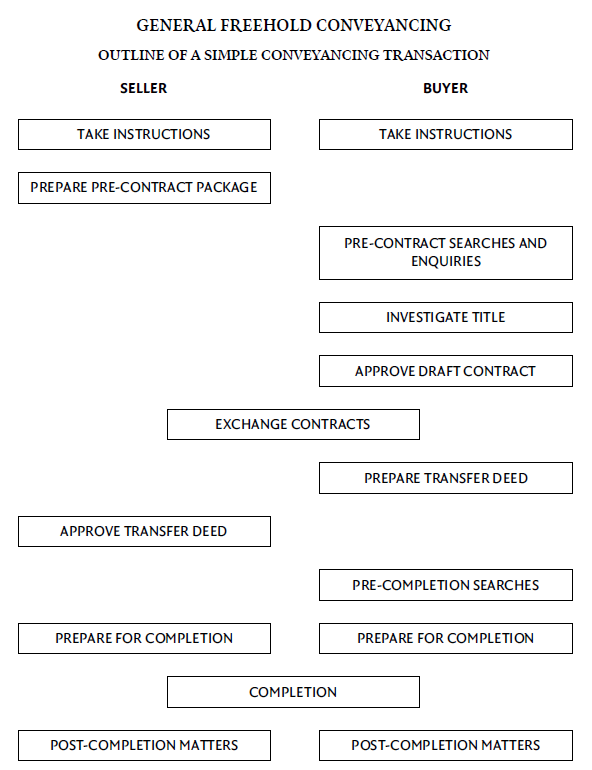
\includegraphics{C:/Users/shiva/Filen/MEGA/LegalPracticeCourse/conveyancing-outline.png}

\hypertarget{land-law}{%
\section{Land Law}\label{land-law}}

\hypertarget{freehold-covenants}{%
\subsection{Freehold Covenants}\label{freehold-covenants}}

\begin{itemize}
\tightlist
\item
  Covenantor and covenantee
\item
  Positive or restrictive

  \begin{itemize}
  \tightlist
  \item
    Hand in pocket test.
  \end{itemize}
\item
  Enforceable as contract between the original parties

  \begin{itemize}
  \tightlist
  \item
    But want it to be enforceable against the current owner of the land.
  \end{itemize}
\item
  May be enforceable against successors in title.
\end{itemize}

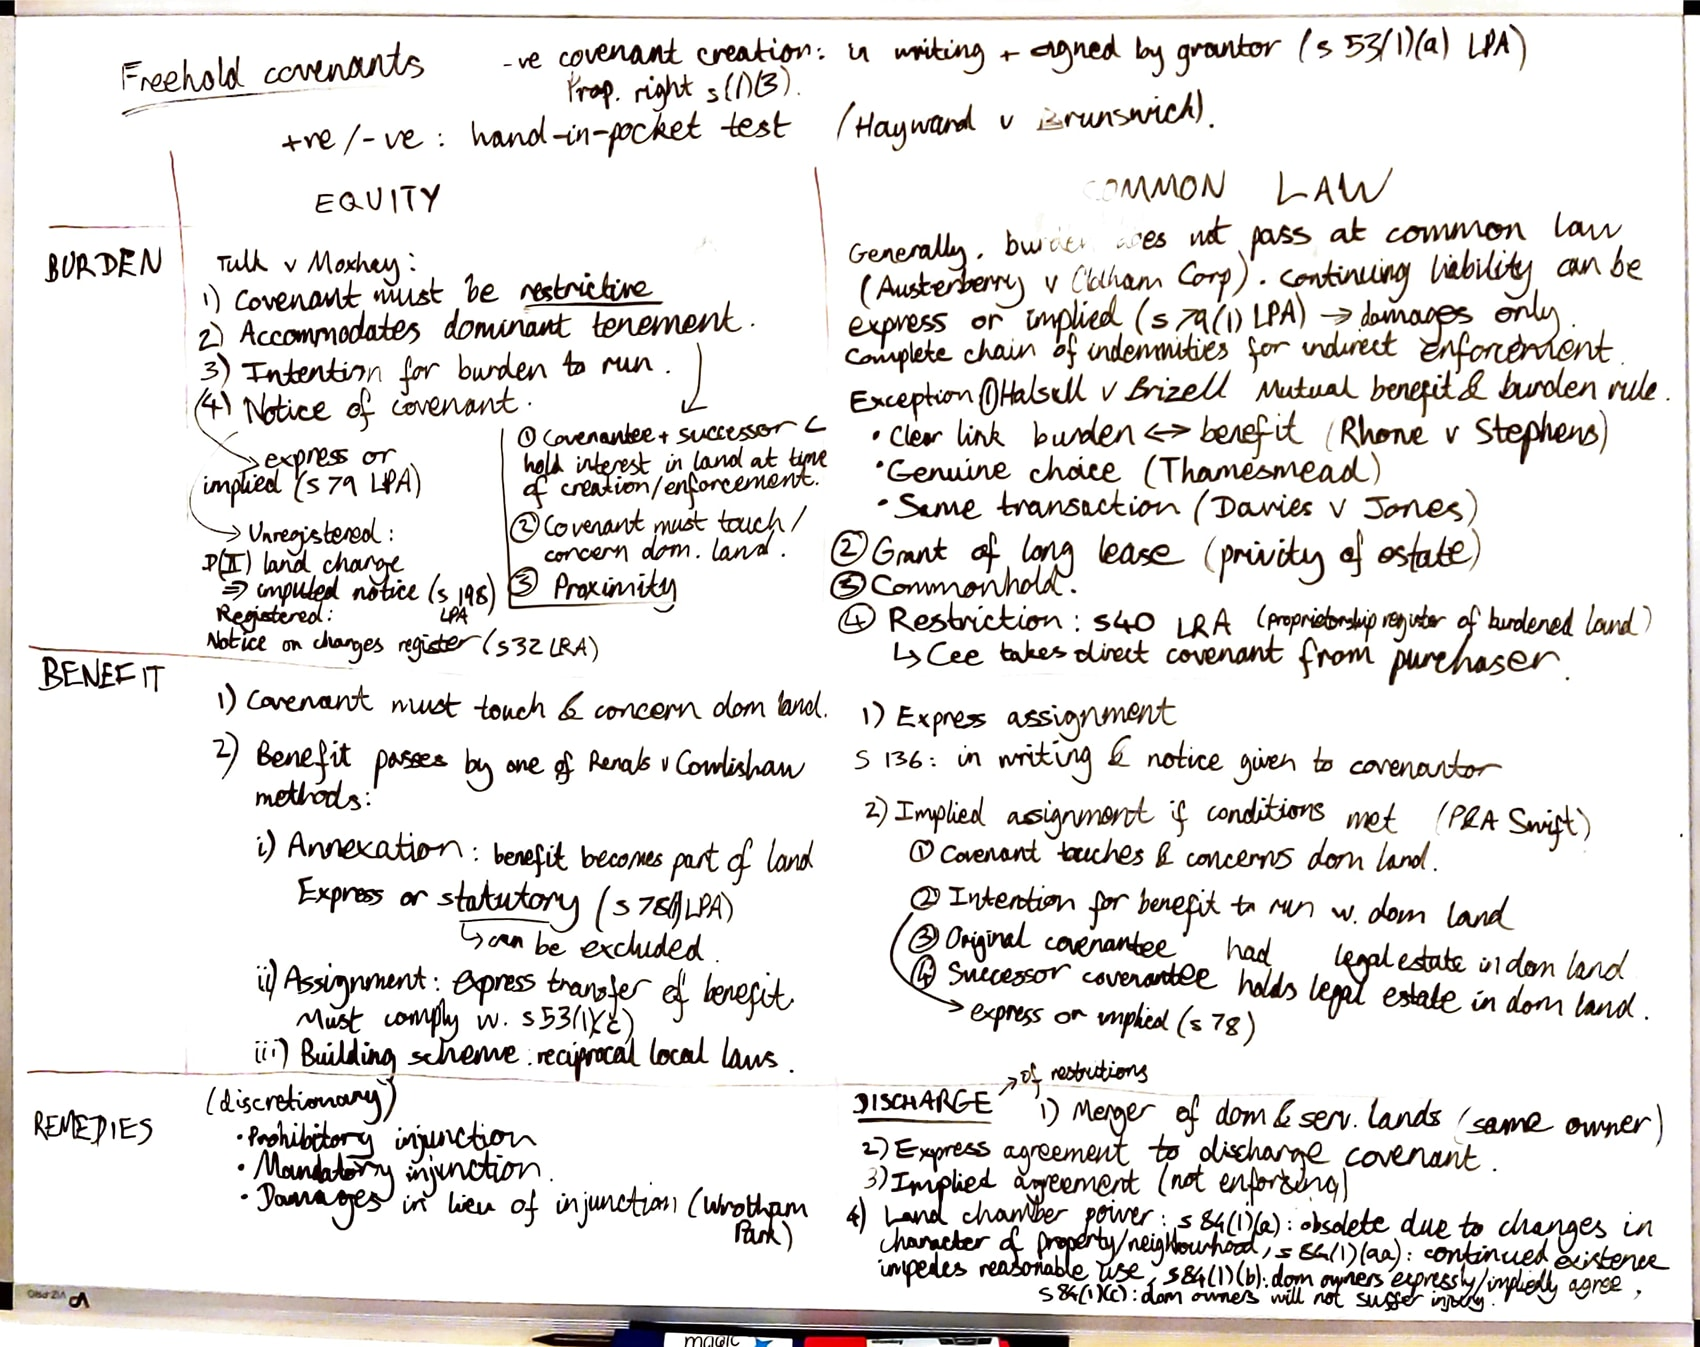
\includegraphics{C:/Users/shiva/Filen/MEGA/LegalPracticeCourse/freehold covenants_1.jpg}

\hypertarget{introduction-1}{%
\subsubsection{Introduction}\label{introduction-1}}

A covenant is a promise relating to land. Covenants are usually
contained in a transfer deed made when someone sells part of their land
and wants to control what happens on the land sold off. The seller makes
it part of the sale deal that the buyer will enter into covenants which
have the effect of preserving the amenity and value of the land retained
by the seller. Covenants are in effect a means of private control of
land use.

\hypertarget{context}{%
\paragraph{Context}\label{context}}

This is an area of law which arose at the time of the industrial
revolution in the mid-nineteenth century, when landowners were selling
part of their land for industrial and housing development. In order to
preserve the quality and value of what they had left, the landowners
imposed strict covenants as to what could and could not be done on the
land sold off.

\begin{env-de3101d4-f08b-48eb-bc0e-2fa06f3bcf8e}

Example

For example, they might require the buyer to covenant not to develop the
land without the consent of the seller; or may covenant not to use the
land for manufacturing or industrial purposes; or may covenant to use it
for residences, maybe even restricting the number of houses which can be
built on the land. All of these covenants have the effect of preserving
the value of the seller's retained land because they eliminate the
possibility of the adjoining land being used for a purpose which would
reduce the attractiveness, quality and value of the retained land.

\end{env-de3101d4-f08b-48eb-bc0e-2fa06f3bcf8e}

\hypertarget{terminology}{%
\paragraph{Terminology}\label{terminology}}

\begin{longtable}[]{@{}ll@{}}
\toprule()
Term & Definition \\
\midrule()
\endhead
Covenantee & Person who has sold part of their land and has required the
buyer to enter into the covenant. The covenantee is the person entitled
to sue for breach of covenant. \\
Dominant land & Land owned by the covenantee. \\
Covenantor & Person giving the promise and entering into the covenant.
Often referred to as the grantor of the covenant. Can be sued if
covenant is breached. \\
Servient land & Land owned by the covenantor which is burdened by the
covenant. \\
\bottomrule()
\end{longtable}

Almost inevitably, the dominant and servient land will be sold or
transferred to new owners at some point. When the dominant land is
transferred, the new owner is successor-in-title to the original
covenantee, and is known as the successor covenantee. If the relevant
rules have been observed, that person now has the ability to sue for
breach of covenant. The rules on the burden of a covenant passing to a
successor covenantor are complex.

\hypertarget{positive-and-restrictive-covenants}{%
\subsubsection{Positive and Restrictive
Covenants}\label{positive-and-restrictive-covenants}}

Covenants impose two main types of obligation: positive and negative. A
positive covenant is a promise actively to do something.

\begin{env-de3101d4-f08b-48eb-bc0e-2fa06f3bcf8e}

Example

The promise to do something will usually involve spending money: it
could be a direct obligation to pay money, perhaps towards the upkeep of
a shared facility such as a driveway, a parking area, or a communal
garden. The covenant could involve payment of money, which is not
directly stated. For example, there could be an obligation for the
covenantor to maintain a fence, a wall, or a roof; or to paint the
exterior of a house every two years. This will inevitably involve some
sort of expenditure. But it does not necessarily involve money. A
covenant to keep a garden tidy may not involve expenditure but it does
require time and effort to fulfil and is therefore a positive
obligation.

\end{env-de3101d4-f08b-48eb-bc0e-2fa06f3bcf8e}

A negative or, more properly, a restrictive covenant is a promise not to
do a specific thing on the land. It restricts the use of the land in
some way.

\begin{env-de3101d4-f08b-48eb-bc0e-2fa06f3bcf8e}

Example

There are many examples: not to use land for industrial, or retail, or
hot food takeaways, or manufacturing; not to build above a certain
height, or above a certain density of housing; not to install a window
overlooking the dominant land...

\end{env-de3101d4-f08b-48eb-bc0e-2fa06f3bcf8e}

\begin{quote}
`Only such a covenant as can be complied with without expenditure of
money will be enforced' against a successor covenantor.'\\
Lindley LJ, Haywood v Brunswick Permanent Benefit Building Society
(1881) 8 QBD 403
\end{quote}

\begin{env-9a1d7316-f242-42ab-b216-19df5e12c935}

Hand in pocket test

The test for identifying whether a covenant is positive or restrictive
is set out in Haywood v Brunswick Permanent Benefit Building Society
(1881) 8 QBD 403

This is known as the `hand in pocket' test. If covenantors have to put
their hands in their pockets to find money to spend to perform the
covenant, it is positive.

`Time is money' so any covenant which requires expenditure of money,
effort or time falls within the definition of positive covenants'.

\end{env-9a1d7316-f242-42ab-b216-19df5e12c935}

Deciding whether a covenant is positive or restrictive is a matter of
looking at the substance not form: look beyond the words used and ask
`what is the essence of the obligation?'

Mixed covenants, which impose positive and restrictive obligations, can
be interpreted in one of two ways:

\begin{enumerate}
\tightlist
\item
  as separate covenants or
\item
  as one obligation with a condition attached
\end{enumerate}

\hypertarget{separate-covenants}{%
\paragraph{Separate Covenants}\label{separate-covenants}}

Shepherd Homes Ltd v Sandham (No 2) {[}1971{]} 2 All ER 1267

This approach can be taken if the positive and restrictive aspects of
the obligation can be separated to create two separate `stand alone'
covenants; one positive and one restrictive.

\begin{env-de3101d4-f08b-48eb-bc0e-2fa06f3bcf8e}

Example

A covenant to paint the exterior of a building every two years and not
to paint the front door red\\
This covenant can be split.

\begin{itemize}
\tightlist
\item
  To paint the exterior every two years: positive.
\item
  Not to paint the front door red: restrictive.
\end{itemize}

\end{env-de3101d4-f08b-48eb-bc0e-2fa06f3bcf8e}

\hypertarget{one-obligation-with-condition}{%
\paragraph{One Obligation with
Condition}\label{one-obligation-with-condition}}

Powell v Hemsley {[}1909{]} 2 Ch 252

This approach is taken if the mixed covenant cannot be split into two
separate obligations. The covenant is interpreted as being overall
positive or restrictive, depending on whether it obliges the covenantor
to do or not do something.

The additional element, which cannot stand alone as a covenant, is
viewed as being simply a condition attached to an overall positive or
restrictive obligation.

\begin{env-de3101d4-f08b-48eb-bc0e-2fa06f3bcf8e}

Example

A covenant not to build on the servient land without the consent of the
dominant owner. This covenant cannot be split.

\begin{itemize}
\tightlist
\item
  Not to build' is the main obligation: restrictive covenant.
\item
  `Without consent' is not a stand alone obligation. Seeking consent
  only operates as part of the main obligation: positive condition
  attached.
\end{itemize}

\end{env-de3101d4-f08b-48eb-bc0e-2fa06f3bcf8e}

\hypertarget{enforceability-of-freehold-covenants}{%
\subsubsection{Enforceability of Freehold
Covenants}\label{enforceability-of-freehold-covenants}}

Suppose there is a covenant between A and B. Suppose A sells the
dominant land to C and B sells the servient land to D. There is now no
direct legal relationship between C and D; there is no contract between
them. This presents a problem for enforceability.

To enforce such a covenant, it must be shown that:

\begin{itemize}
\tightlist
\item
  C has the benefit of the covenant, and
\item
  D has the burden of the covenant.
\end{itemize}

There are two sets of rules which must be applied to see whether the
benefit and burden have passed to the successor covenantee and
covenantor, respectively. One set is the rules of equity, and the other
is the common law rules. It is vitally important that these rules are
not muddled or used on a mix and match basis. It is not possible, for
example, to apply the common law rules to pass the benefit to C and the
rules of equity to pass the burden to D. If the equity rules are applied
to pass the burden, then they must be applied to pass the benefit.

\hypertarget{equitable-rules-burden}{%
\subsubsection{Equitable Rules: Burden}\label{equitable-rules-burden}}

As a general rule, the burden of a covenant does not pass to a successor
at common law: Austerberry v Oldham Corporation {[}1885{]} AC 29 ChD
750. This means that at common law, the covenant is unenforceable
against a successor in title to the covenantor.

Equity has developed rules which allow the burden of certain covenants
to pass to successors, which allows the covenant to be enforced direct
against the person in breach. It is equity's intervention which has
created the proprietary right, which we know as the \textbf{restrictive
covenant}.

The formalities for creating a restrictive covenant are set out in
\href{https://www.legislation.gov.uk/ukpga/Geo5/15-16/20/section/53}{LPA
1925, s 53(1)(a)}: in writing and signed by the grantor. A restrictive
covenant is a proprietary right:
\href{https://www.legislation.gov.uk/ukpga/Geo5/15-16/20/section/1}{LPA
1925, s 1(3)}.

\begin{env-9a1d7316-f242-42ab-b216-19df5e12c935}

Tulk v Moxhay rules

The equitable rules began with the case of Tulk v Moxhay (1848) 2 Ph
774. There are 4 aspects to the rule:

\begin{enumerate}
\tightlist
\item
  The covenant must be restrictive
\item
  It must accommodate the dominant tenement
\item
  There must be intention for the burden to run
\item
  There must be notice of the covenant
\end{enumerate}

\end{env-9a1d7316-f242-42ab-b216-19df5e12c935}

\hypertarget{the-covenant-must-be-restrictive}{%
\paragraph{The Covenant Must Be
Restrictive}\label{the-covenant-must-be-restrictive}}

In Rhone v Stephens {[}1994{]} AC 310 Lord Templemen said

\begin{quote}
`For over 100 years it has been accepted law that equity will enforce
negative covenants against freehold land but has no power to enforce
positive covenants against successors in title of the land'.
\end{quote}

This means that to enforce a covenant in equity, it must be shown that
the substance of the covenant is restrictive. If a covenant is positive,
then the common law rules will apply to its enforcement. Positive
covenants can only be enforced at common law.

\hypertarget{accommodate-dominant-tenement}{%
\paragraph{Accommodate Dominant
Tenement}\label{accommodate-dominant-tenement}}

There are three aspects:

\begin{enumerate}
\tightlist
\item
  The covenantee and successor covenantee must hold an interest in land
  at the time of creation and enforcement.

  \begin{itemize}
  \tightlist
  \item
    The original covenantee and successors must have retained an
    interest in dominant land at the time of creation and enforcement of
    the covenant.
  \item
    LCC v Allen {[}1914{]} 3 KB 642.
  \end{itemize}
\item
  The covenant must touch and concern the dominant land

  \begin{itemize}
  \tightlist
  \item
    This means that it is the land, and not simply the dominant owner,
    which must benefit from the covenant.
  \item
    P\&A Swift Investments Ltd v Combined English Stores Group plc
    {[}1989{]} AC 632
  \end{itemize}
\item
  The dominant land and the servient land must be in proximity.

  \begin{itemize}
  \tightlist
  \item
    The two pieces of land must be near to each other, although they do
    not need to share a common boundary, or be directly next to each
    other
  \item
    Bailey v Stephens (1862) 12 CB (NS) 91
  \end{itemize}
\end{enumerate}

\hypertarget{intention-for-burden-to-run}{%
\paragraph{Intention for Burden to
Run}\label{intention-for-burden-to-run}}

This can be shown expressly or impliedly.

\hypertarget{expressly}{%
\subparagraph{Expressly}\label{expressly}}

The covenant is worded in such a way as to make it clear that successors
are to be bound:

\begin{env-de3101d4-f08b-48eb-bc0e-2fa06f3bcf8e}

Example

\begin{itemize}
\tightlist
\item
  `A hereby covenants with B for himself and his successors in title to
  land known as\ldots' or
\item
  `A hereby covenants with the intention of binding land known as\ldots'
\end{itemize}

\end{env-de3101d4-f08b-48eb-bc0e-2fa06f3bcf8e}

\hypertarget{impliedly}{%
\subparagraph{Impliedly}\label{impliedly}}

\href{https://www.legislation.gov.uk/ukpga/Geo5/15-16/20/section/79}{LPA
1925, s 79} states that a covenant relating to land shall be deemed to
be made by the covenantor on behalf of his successors in title, unless a
contrary intention is expressed. The section makes the original
covenantor liable for all breaches of covenant by any person who holds
the land after the original covenantor has parted with it. It does not
pass the burden of the covenant.

\hypertarget{there-must-be-notice-of-the-covenant}{%
\subparagraph{There Must Be Notice of the
Covenant}\label{there-must-be-notice-of-the-covenant}}

Unregistered Land

The covenant must be entered as a D(ii) Land Charge
(\href{https://www.legislation.gov.uk/ukpga/1972/61/section/2}{LCA 1972
s 2(5)(ii)}). If so, a purchaser will be deemed to have notice of the
covenant
(\href{https://www.legislation.gov.uk/ukpga/Geo5/15-16/20/section/198}{LPA
1925, s 198}). If the covenant has not been protected by entering a
D(ii) Land Charge, a purchaser of a legal estate will take the land free
of the covenant, they will not be bound
(\href{https://www.legislation.gov.uk/ukpga/1972/61/section/4}{LCA 1972,
s 4(6)}).

However, if the successor covenantor has been gifted or inherited the
estate, they will still be bound despite the fact it has not been
correctly protected. Whether the successor covenantor is deemed to have
notice of the covenant depends on whether it has been properly protected
by registration.

Registered Land

The covenant must be protected by the entry of a notice in the charges
register of the servient title
(\href{https://www.legislation.gov.uk/ukpga/2002/9/section/32}{LRA 2002,
s 32}). If so, everyone, including a purchaser for valuable
consideration, will be bound
(\href{https://www.legislation.gov.uk/ukpga/2002/9/section/29}{s 29(2)
LRA 2002}).

If not, a purchaser for valuable consideration will take the land free
of it and would not be bound
(\href{https://www.legislation.gov.uk/ukpga/2002/9/section/29}{s 29(1)
LRA 2002}), but a successor in title covenantor who has been gifted or
inherited the land (a `volunteer') will still be bound
(\href{https://www.legislation.gov.uk/ukpga/2002/9/section/28}{s 28 LRA
2002}).

\hypertarget{equitable-rules-benefit}{%
\subsubsection{Equitable Rules: Benefit}\label{equitable-rules-benefit}}

The various ways in which the benefit of a covenant can pass to a
successor covenantee are set out.

\hypertarget{context-1}{%
\paragraph{Context}\label{context-1}}

If a successor covenantee wishes to enforce a breach against a successor
covenantor direct, two things must be shown:

\begin{enumerate}
\tightlist
\item
  that the burden of the covenant has passed to the successor covenantor
  in equity and
\item
  that the benefit has passed to the successor covenantee in equity.
\end{enumerate}

It is not enough to show that the burden has passed in equity and the
benefit passes at common law. If an equitable remedy is required, both
the benefit and burden must pass in equity: the rules go hand in hand.

There are two elements which must be fulfilled for the benefit to pass
in equity:

\begin{enumerate}
\tightlist
\item
  The covenant must `touch and concern' the dominant land
\item
  The benefit must pass by one of the methods in Renals v Cowlishaw
  (1878) 9 ChD 125
\end{enumerate}

\hypertarget{methods-of-passing-the-benefit}{%
\paragraph{Methods of Passing the
Benefit}\label{methods-of-passing-the-benefit}}

The case of Renals v Cowlishaw (1878) 9 ChD 125 sets out 3 ways in which
the benefit of a covenant can pass to a successor covenantee in equity:

\begin{enumerate}
\tightlist
\item
  Annexation
\item
  Assignment
\item
  Building Scheme
\end{enumerate}

\hypertarget{annexation}{%
\subparagraph{Annexation}\label{annexation}}

\begin{env-615494ee-4c11-425d-a24a-676608cc22a4}

Definition

Annexation occurs when the covenant is made in such a way that the
benefit becomes a permanent part of the dominant land itself. It
therefore passes automatically when the dominant land is sold, without
being specifically mentioned in the transfer deed.

\end{env-615494ee-4c11-425d-a24a-676608cc22a4}

Annexation occurs in one of two main ways:

\begin{enumerate}
\item
  Express annexation

  \begin{itemize}
  \tightlist
  \item
    The words of the covenant are sufficient to make the benefit part
    and parcel of the dominant land from the outset.
  \item
    This occurs where the express words of the covenant make it clear
    that the original parties intend the benefit to become part of the
    dominant land, rather than simply a personal advantage to the
    covenantee.
  \item
    In Rogers v Hosegood {[}1900{]} 2 Ch 388 a covenant made `for the
    benefit of the owners and successors in title' to named land, which
    was enough to demonstrate express annexation.
  \item
    In Renals v Cowlishaw (1878) 9 ChD 125 a covenant stated to be made
    with the covenantees, their heirs, executors and assignees was not
    enough to show express annexation because the benefit was stated to
    be for people, not for land.
  \end{itemize}
\item
  Statutory annexation
  \href{https://www.legislation.gov.uk/ukpga/Geo5/15-16/20/section/78}{LPA
  1925, s 78}

  \begin{itemize}
  \tightlist
  \item
    LPA 1925, s 78(1) was interpreted in the case of Federated Homes v
    Mill Lodge Properties Ltd {[}1980{]} 1 WLR 594 as providing that a
    covenant relating to any land of the covenantee shall be deemed to
    be made with the covenantee and his successors in title of the land
    intended to be benefitted.
  \item
    This would appear to make express words of annexation unnecessary,
    as it seems to make annexation automatic.
  \item
    However, Roake v Chadha {[}1984{]} 1 WLR 40 held that s 78(1) can be
    expressly excluded. This can happen if an alternative method of
    passing the benefit is stipulated in the original transfer deed.
  \end{itemize}
\end{enumerate}

\begin{env-9843ce55-0506-497d-95ba-03a690b05b3c}

s 78(1) LPA 1925

A covenant relating to any land of the covenantee shall be deemed to be
made with the covenantee and his successors in title and the persons
deriving title under him or them, and shall have effect as if such
successors and other persons were expressed.

\end{env-9843ce55-0506-497d-95ba-03a690b05b3c}

\hypertarget{assignment}{%
\subparagraph{Assignment}\label{assignment}}

\begin{env-615494ee-4c11-425d-a24a-676608cc22a4}

Definition

Assignment is the express transfer of the benefit of a covenant
alongside a transfer of the dominant land.

\end{env-615494ee-4c11-425d-a24a-676608cc22a4}

This occurs where the benefit of the covenant has not been annexed at
the outset. The benefit can nevertheless be assigned when the dominant
land is transferred. As the benefit exists separately from the land
itself, it is treated as a separate interest in the land and must be
transferred every time the land is transferred.

The separate assignment of the benefit must comply with the formalities
in
\href{https://www.legislation.gov.uk/ukpga/Geo5/15-16/20/section/53}{LPA
1925, s 53(1)(c)}: in writing and signed by the person transferring the
benefit.

\hypertarget{building-scheme}{%
\subparagraph{Building Scheme}\label{building-scheme}}

\begin{env-615494ee-4c11-425d-a24a-676608cc22a4}

Definition

If the parties intended to create a scheme of reciprocal local laws in a
building scheme, the benefit of restrictive covenants passes to all new
owners.

\end{env-615494ee-4c11-425d-a24a-676608cc22a4}

When a new housing estate is built, all houses are sold subject to the
same covenants. New owners who wish to enforce a covenant against a
neighbour may struggle to show that the benefit of a particular covenant
has passed to them.

Building schemes resolve this problem relating to restrictive covenants
only. If the conditions of a building scheme are met, the covenants are
treated as a set of by-laws enforceable by and against all owners. It is
not necessary to show specifically that the benefit of a particular
covenant has passed to a claimant.

\begin{env-9a1d7316-f242-42ab-b216-19df5e12c935}

Building scheme

The conditions are set out in Ellison v Reacher {[}1908{]} 2 Ch 374:

\begin{enumerate}
\tightlist
\item
  All buyers buy from the same seller
\item
  The seller divided the estate into plots
\item
  The covenants were intended to benefit all plots
\item
  Each buyer buys on the understanding that the covenants are intended
  to benefit all plots.
\end{enumerate}

Later cases have interpreted these rules as \textbf{guidelines} rather
than strict requirements.

A court will need to be satisfied that it was the intention of the
parties to create a \textbf{scheme of mutually enforceable obligations}.

\end{env-9a1d7316-f242-42ab-b216-19df5e12c935}

\hypertarget{original-covenantee}{%
\subparagraph{Original Covenantee}\label{original-covenantee}}

When dominant land is sold, the original covenantee technically still
has the benefit of the covenant and can sue on it. This is based on
contractual principles. However, it is highly unlikely that an original
covenantee would wish to enforce a covenant in these circumstances. Even
if action was taken, it is hard to envisage any loss which could be
suffered by an original covenantee who no longer owns the dominant land.

\begin{env-de3101d4-f08b-48eb-bc0e-2fa06f3bcf8e}

Example

A covenant not to build on servient land is of no value to a covenantee
once the dominant land is sold. A breach of the covenant causes the
original covenantee no loss.

\end{env-de3101d4-f08b-48eb-bc0e-2fa06f3bcf8e}

\hypertarget{equitable-remedies}{%
\subsubsection{Equitable Remedies}\label{equitable-remedies}}

As a restrictive covenant is an equitable interest in land, equitable
remedies are available to enforce the breach against the current owner.
These remedies are discretionary, there is no automatic right to them.
The most common remedy for breach of covenant is an injunction.

\begin{longtable}[]{@{}ll@{}}
\toprule()
Term & Definition \\
\midrule()
\endhead
Injunction & An order of the court. \\
Prohibitory injunction & An order requiring a person to refrain from
doing a particular act. \\
Mandatory injunction & An order to undertake a particular act. \\
\bottomrule()
\end{longtable}

Typically, if the breach is threatened or ongoing, the claimant can
apply for a prohibitory injunction, ordering the breach to cease. For
example, if a servient owner is using the burdened land for an
unauthorised use, or is building in breach of covenant, a prohibitory
injunction would be appropriate.

If the breach has already occurred, the claimant can apply for a
mandatory injunction, ordering the person in breach to do something. For
example, if a building has been built in breach of covenant, a mandatory
injunction, ordering the demolition of the building, may be appropriate.

\hypertarget{equitable-principles}{%
\paragraph{Equitable Principles}\label{equitable-principles}}

Equitable remedies are awarded subject to general equitable principles
and maxims. `Delay defeats equity' -- a claimant must not wait too long
before applying for an injunction.

\begin{env-881a4bd6-779e-4404-ae5b-86f77846f864}

Note

A claimant who wishes to apply for an injunction in respect of building
work being carried out in breach of covenant must act immediately. If
the claimant waits until the building is complete and then applies for a
mandatory injunction to knock the building down, the application is
likely to be refused.

\end{env-881a4bd6-779e-4404-ae5b-86f77846f864}

\hypertarget{damages-in-lieu-of-injunctions}{%
\paragraph{Damages in Lieu of
Injunctions}\label{damages-in-lieu-of-injunctions}}

Equitable damages are not awarded as of right. They may be awarded in
lieu of an injunction, as an injunction may be refused where it would be
oppressive to grant it.

Key case: Wrotham Park Estate Co Ltd v Parkside Homes {[}1974{]} 1 WLR
798.

\hypertarget{common-law-rules-burden}{%
\subsubsection{Common Law Rules: Burden}\label{common-law-rules-burden}}

The rule in Tulk v Moxhay (1848) 2 Ph 774 must be used to pass the
burden of a covenant in equity. The first aspect of this is that the
covenant must be negative. Therefore the rules in equity cannot be used
to enforce positive covenants, or indeed any restrictive covenant which
fails any of the other \emph{Tulk v Moxhay} tests. Only the common law
can be used in these circumstances.

It must be shown that the burden has passed to a successor covenantor at
common law, and that the benefit has passed to a successor covenantee at
common law. It is fairly easy to show that the benefit passes at common
law, and for the purposes of this explanation, we will assume that the
benefit has indeed passed to C, enabling C to sue for breach of
covenant.

On the assumption that C can show that the benefit has passed, the
problem as far as C is concerned relates to the burden.

\begin{env-99436a7e-0b1e-438d-960f-947d510b2b61}

Important

It is the general rule at common law that the burden of the covenant
does not pass (Austerberry v Oldham Corporation {[}1885{]} AC 29 ChD
750).

\end{env-99436a7e-0b1e-438d-960f-947d510b2b61}

The effect of the rule is that at common law, C cannot sue D direct as
the burden of the covenant has not passed to D. If the burden of a
covenant does not pass, that does not mean that it disappears. It
remains with the original covenantor permanently. This means that it is
the original covenantor has the burden of the covenant and can be sued.

\hypertarget{continuity}{%
\paragraph{Continuity}\label{continuity}}

This continuity is often found expressly stated in the wording of the
covenant. This can be stated in a variety of ways, but common examples
are:

Example

\begin{itemize}
\tightlist
\item
  `the covenantor covenants for himself, his successors in title and all
  those deriving title under him or them to maintain the boundary
  fence\ldots' or
\item
  `the covenantor covenants that he and his successors in title will
  maintain the boundary fence\ldots' or
\item
  `the covenantor covenants with the intention of binding land known as
  9 Main Street to maintain the boundary fence\ldots'.
\end{itemize}

Even if there is no such express wording in the covenant itself,
\href{https://www.legislation.gov.uk/ukpga/Geo5/15-16/20/section/79}{LPA
1925, s 79(1)} can be used to imply such wording. The case of Topham Ltd
v Earl of Sefton {[}1967{]} 1 AC 50 confirms this. So the effect is that
the original covenantor will be liable for any breach of covenant by
anyone who holds the servient land in the future.

\hypertarget{remedies}{%
\paragraph{Remedies}\label{remedies}}

The problem from the covenantee's point of view is that the only remedy
available against the original covenantor is damages. This may not be
what the covenantee wants. For example, if the successor covenantor has
breached a covenant to maintain a fence, the covenantee wants to force
the successor covenantor to maintain the fence. However, that is not
going to happen as the burden does not pass to the successor covenantor.
If the covenantee sues the original covenantor, the original covenantor
is not in possession of the land and is not therefore in a position to
maintain the fence. Instead, damages may be awarded to the covenantee,
but that simply awards money, and does not solve the essential problem.

Original covenantors may have awards of damages made against them for
breaches of covenant that they did not commit, did not know about, and
had no power to stop. Can the original covenantor do anything to recover
money paid out? The answer to that question depends entirely on whether
the original covenantor (B in this example) was careful (or had a
careful solicitor) when B sold the servient land to D.

As part of the sale process, B should have insisted that D entered into
an indemnity covenant in B's favour. In essence, in the transfer deed, D
promises that, in the event of B being sued for a breach of covenant
after B parts with the servient land, D will reimburse any damages that
B has had to pay out.

This means that if D has to pay out the money for, say, the dilapidated
fence, maybe that will make D more likely to maintain the fence in
future. This is what is meant by `indirect enforcement'. D cannot be
sued direct, but suing B, who then recovers damages paid out from D, may
encourage D to observe the covenant in future.

\hypertarget{chain-of-indemnities}{%
\paragraph{Chain of Indemnities}\label{chain-of-indemnities}}

If the servient land changes hands several times, there is potentially a
`chain of indemnity' as each new servient owner makes an indemnity
covenant with the previous servient owner. In our continuing example,
there is a covenant to maintain a boundary fence. B may sell the
servient land to D, who sells to F, who sells to H. H breaches the
covenant and lets the fence fall down in places. As the maintenance
covenant is positive, B is sued for the breach, and pays out damages. As
D has made an indemnity covenant with B when D bought, B can recover the
sums paid out from D. As F has made an indemnity covenant with D when F
bought, D can recover any sums paid out to B from F. Note that B cannot
sue F direct as there is no direct covenant between B and F.

\hypertarget{shortcomings}{%
\paragraph{Shortcomings}\label{shortcomings}}

In this example, in the transfer from F to H, F did not ask H to enter
into an indemnity covenant. This means that if H breaches covenant, B
will be sued and can recover from D; D in turn can recover from F, but
the chain of indemnity is then broken and F cannot recover from H. As H
has not had to pay anything out, there is no incentive for H to stop
breaching covenant. This is one of the problems with indemnity chains.

Moreover, F may have been declared bankrupt; or may have died; or may
not be traceable. In that case, there is no practical possibility of D
recovering any outlay, even though technically, everything has been done
correctly.

\hypertarget{exceptions-to-the-common-law-rule}{%
\subsubsection{Exceptions to the Common Law
Rule}\label{exceptions-to-the-common-law-rule}}

\hypertarget{mutual-benefit-and-burden}{%
\paragraph{Mutual Benefit and Burden}\label{mutual-benefit-and-burden}}

Halsall v Brizell {[}1957{]} Ch 169 gives a limited exception to the
general rule, enabling the burden of a covenant to pass to a successor
covenantor at common law.

It is known as the \textbf{`mutual benefit and burden' rule}, and
applies where the covenantee grants to the covenantor a benefit in the
nature of an easement, and imposes a connected burden.

For example, in the transfer deed selling part of a piece of land, a
covenantee grants the covenantor a right to park on the covenantee's
land. In the same deed, the covenantor covenants to contribute to the
cost of maintaining the parking area.

In a case like this, a successor covenantor cannot take the benefit of
parking but avoid payment by relying on the basic common law rule of the
burden not passing.

\hypertarget{refinements}{%
\subparagraph{Refinements}\label{refinements}}

The rules has been refined in subsequent cases:

\begin{longtable}[]{@{}ll@{}}
\toprule()
Case & Ratio \\
\midrule()
\endhead
Rhone v Stephens {[}1994{]} 2 AC 310 & There must be a clear link
between the burden and the benefit. There is no general principle that
someone who takes a benefit under a deed must submit to any burden which
it imposes. \\
Thamesmead Town Ltd v Allotey (1998) 3 EGLR 97 & There must be a genuine
choice as to whether or not to take the benefit. This choice can be
theoretical. The condition of discharging the covenanted burden must be
relevant to the exercise of the right (more than incidental). \\
Davies v Jones {[}2009{]} EWCA Civ 1164 & The benefit and burden must
have been conferred in the same transaction. \\
\bottomrule()
\end{longtable}

\hypertarget{grant-of-long-lease}{%
\subparagraph{Grant of Long Lease}\label{grant-of-long-lease}}

One way of side-stepping the rule that the burden of a freehold covenant
will not pass to a successor covenantor is to dispose of the land by way
of long lease. All covenants in leases except personal ones are
enforceable by and against successors in title via the doctrine of
privity of estate.

\hypertarget{commonhold-development}{%
\subparagraph{Commonhold Development}\label{commonhold-development}}

Commonhold is a way of holding land in units such as blocks of flats.
Each unit owner has obligations, such as contributing towards the
maintenance of each unit. The rights and obligations attach by statute
(\href{https://www.legislation.gov.uk/ukpga/2002/15/contents}{Commonhold
and Leasehold Reform Act 2002}) to each unit, so all obligations are
enforceable against all unit holders at all times.

Unfortunately, commonhold has not proved a popular way of holding land.

\hypertarget{restriction-s-40-lra-2002}{%
\subparagraph{Restriction: S 40 LRA
2002}\label{restriction-s-40-lra-2002}}

\begin{env-881a4bd6-779e-4404-ae5b-86f77846f864}

Note

This is the most commonly used way of making the burden of positive
covenants run on registered land.

\end{env-881a4bd6-779e-4404-ae5b-86f77846f864}

A covenantee can put a restriction on the \textbf{proprietorship
register of the burdened land}. This states that no transfer of the
burdened land can be registered without the consent of the covenantee.
As a condition of giving consent to the transaction, the covenantee
takes a direct covenant from the purchaser of the burdened land.

In the new covenant, the new owner promises to observe the covenants in
the original transfer. This creates a new privity of contract between
the covenantee and purchaser, enabling direct enforcement of the
covenants.

\hypertarget{other-methods}{%
\subparagraph{Other Methods}\label{other-methods}}

\begin{itemize}
\tightlist
\item
  Reserving a rentcharge annexed to a right of entry
\item
  Reserving a freehold right of entry
\item
  Less commonly used.
\end{itemize}

\hypertarget{common-law-rules-benefit}{%
\subsubsection{Common Law Rules:
Benefit}\label{common-law-rules-benefit}}

The original covenantee can enforce a covenant as a matter of contract
law. If the dominant land is sold, the successor covenantee must show
that the benefit has passed to it at common law.

This enables the successor covenantee to enforce the covenant either
against the original covenantor, or (in limited circumstances) against
the successor covenantor.

There are two ways the benefit can pass at common law:

\hypertarget{express-assignment}{%
\paragraph{Express Assignment}\label{express-assignment}}

Under normal contractual principles, the benefit of a covenant can be
expressly assigned to a successor.

\href{https://www.legislation.gov.uk/ukpga/Geo5/15-16/20/section/136}{LPA
1925, s 136} requires the assignment must be in writing and express
notice of the assignment must be given to the covenantor. This is to
ensure that the covenantor realises that a new person is in a position
to enforce the covenant.

\hypertarget{implied-assignment}{%
\paragraph{Implied Assignment}\label{implied-assignment}}

Where there is no express assignment, the benefit of a covenant may pass
to a successor covenantee if certain conditions are met. This involves
the benefit automatically passing every time the land is transferred, as
long as the conditions are met.

\begin{env-9a1d7316-f242-42ab-b216-19df5e12c935}

Implied assignment

The conditions of implied assignment are set out in P\&A Swift
Investments Ltd v Combined English Stores Group plc {[}1989{]} AC 632:

\begin{enumerate}
\tightlist
\item
  The covenant must touch and concern the land
\item
  There must have been an intention that the benefit should run with the
  dominant land
\item
  The original covenantee must have a legal estate in the dominant land
\item
  The successor covenantee must hold a legal estate in the dominant land
\end{enumerate}

\end{env-9a1d7316-f242-42ab-b216-19df5e12c935}

\hypertarget{the-covenant-must-touch-and-concern-the-land}{%
\paragraph{The Covenant Must Touch and Concern the
Land}\label{the-covenant-must-touch-and-concern-the-land}}

The covenant must benefit the dominant land itself, it must affect the
nature, quality, use or value of the land. It must not be expressed to
be personal and should only benefit the dominant owner for the time
being, so that, if separated from the land, it ceases to be of any
advantage to them.

\begin{env-de3101d4-f08b-48eb-bc0e-2fa06f3bcf8e}

Example

A covenant to maintain a house on the burdened land does touch and
concern the dominant land as it preserves the quality of the environment
and therefore the value of the dominant land.

\end{env-de3101d4-f08b-48eb-bc0e-2fa06f3bcf8e}

\hypertarget{intention-that-benefit-runs-with-dominant-land}{%
\paragraph{Intention That Benefit Runs with Dominant
Land}\label{intention-that-benefit-runs-with-dominant-land}}

Intention of the parties can be shown expressly or impliedly through
statute.

If there is no express intention,
\href{https://www.legislation.gov.uk/ukpga/Geo5/15-16/20/section/78}{LPA
1925, s 78} implies an intention for the benefit to pass unless it is
expressly excluded.

\begin{env-de3101d4-f08b-48eb-bc0e-2fa06f3bcf8e}

Example

A covenant drafted `for the benefit of land known as 5 High Street' or
`with the covenantee and successors in title to land known as 5 High
Street' shows express intention

\end{env-de3101d4-f08b-48eb-bc0e-2fa06f3bcf8e}

The original covenantee must have a legal estate in the dominant land,
and the successor covenantee must hold a legal estate in the dominant
land. The original covenantee must have owned a legal estate when the
covenant was made, and that the successor must own a legal estate at the
time of enforcement.

The legal estate does not need to be of the same nature: Smith and
Snipes Hall Farm Ltd v River Douglas Catchment Board {[}1949{]} 2 KB
500.

In that case, the original covenantee held a freehold and the successor
held a leasehold. The successor was held to be entitled to the benefit
of the covenant and could therefore enforce it.

\hypertarget{ending-freehold-covenants}{%
\subsubsection{Ending Freehold
Covenants}\label{ending-freehold-covenants}}

The methods by which a freehold covenant can be brought to an end are
discharge, modification and release.

\hypertarget{problem-with-old-covenants}{%
\paragraph{Problem with Old
Covenants}\label{problem-with-old-covenants}}

Restrictive covenants, once validly granted, last forever. Over time,
these can become obsolete and can unduly restrict the use of the
servient land.

\begin{env-de3101d4-f08b-48eb-bc0e-2fa06f3bcf8e}

Example

A covenant not to build on land might have benefitted the dominant
tenement whilst that land was used for residential purposes, but no
longer does if the dominant land is now a factory.

\end{env-de3101d4-f08b-48eb-bc0e-2fa06f3bcf8e}

There are various ways in which a covenant can be discharged or
modified. Discharge if a covenant means that it is no longer valid.
Modification of a covenant means that the scope of the covenant is
altered, but it is not completely invalidated.

\hypertarget{methods-of-dischargingmodifying-covenants}{%
\paragraph{Methods of discharging/modifying
Covenants}\label{methods-of-dischargingmodifying-covenants}}

A covenant will be automatically be discharged if the same person
becomes the owner of both the dominant and servient land: Re Tiltwood,
Sussex {[}1978{]} Ch 269. This is known as merger. A dominant owner may
expressly agree to discharge the covenant and will enter into a formal
release of covenant, usually in return for a payment.

The release must be made by deed. Alternatively, the dominant owner may
impliedly agree to discharge the covenant by doing nothing when the
covenant is being breached openly.

\hypertarget{statutory-discharge-or-modification-of-covenants}{%
\paragraph{Statutory Discharge or Modification of
Covenants}\label{statutory-discharge-or-modification-of-covenants}}

The dominant owner could hold the servient owner to ransom by asking for
a large sum of money to discharge an obsolete covenant.

To avoid this, the servient owner can apply to the Tribunals
\textgreater{} Upper Tribunal (Lands Chamber) for the discharge or
modification of any covenant.

\href{https://www.legislation.gov.uk/ukpga/Geo5/15-16/20/section/84}{Law
of Property Act 1925, s 84(1)} gives the Lands Chamber the power `wholly
or partially to discharge or modify any\ldots{} restriction'.

\begin{env-7ede146d-a28c-46fa-985d-64c388b7528b}

Warning

This provision only applies to restrictive covenants.

\end{env-7ede146d-a28c-46fa-985d-64c388b7528b}

\begin{env-9843ce55-0506-497d-95ba-03a690b05b3c}

\href{https://www.legislation.gov.uk/ukpga/Geo5/15-16/20/section/84}{LPA
1925, s 84(1)(a)}

A servient owner may apply to the tribunal for a declaration to
discharge or modify a covenant on the basis that the covenant has become
obsolete due to changes in the character of the property or
neighbourhood.

\end{env-9843ce55-0506-497d-95ba-03a690b05b3c}

\begin{env-de3101d4-f08b-48eb-bc0e-2fa06f3bcf8e}

Example

A covenant to use property only as a residence may be obsolete if the
surrounding area is now business, retail of mixed use.

\end{env-de3101d4-f08b-48eb-bc0e-2fa06f3bcf8e}

\href{https://www.legislation.gov.uk/ukpga/Geo5/15-16/20/section/84}{s
84(1)(aa)} enables an application to be made on the basis that the
covenant impedes reasonable use of the servient land. The applicant must
show either that the covenant confers no practical value, or that it is
contrary to public interest. The tribunal must be satisfied that
financial compensation would be adequate for the dominant owner.

\begin{env-de3101d4-f08b-48eb-bc0e-2fa06f3bcf8e}

Example

A covenant restricting the density of houses on a plot may confer no
practical value on the dominant land if that land is itself densely
developed.

\end{env-de3101d4-f08b-48eb-bc0e-2fa06f3bcf8e}

S 84(1)(b) applies where the dominant owners have agreed, expressly or
impliedly, to discharge.

\begin{env-de3101d4-f08b-48eb-bc0e-2fa06f3bcf8e}

Example

An application here may be appropriate where the parties have expressly
agreed a release in principle, or where the dominant owner has tolerated
a long-term breach. In this instance, the tribunal will decide the level
of compensation to be paid, thereby preventing the dominant owner
holding the servient owner to ransom.

\end{env-de3101d4-f08b-48eb-bc0e-2fa06f3bcf8e}

S 84(1)(c) enables an application to be made where discharge if a
covenant will not 'injure' the dominant owners.

This provision means that the tribunal can override spurious or
frivolous objections.

However, the tribunal has a balancing act to do: on the one hand it will
be wary of discharging covenants on this basis simply because discharge
will not injure the current dominant owner. On the other hand it will
have regard to social and economic concerns: the wider public interest
rather than the interest of one particular dominant owner.

\hypertarget{easements}{%
\subsection{Easements}\label{easements}}

\begin{itemize}
\tightlist
\item
  Positive or negative
\item
  Better than a licence (which is just a personal permission to do
  something which would otherwise be trespass).
\item
  Right in rem!
\item
  As of right, not with permission.
\item
  Expressly Created

  \begin{itemize}
  \tightlist
  \item
    Created by deed (s 52 LPA 1925)
  \item
    With correct formalities
  \item
    Granted forever or for fixed period
  \item
    Registered against both title.
  \end{itemize}
\item
  Implied Grant or Reservation

  \begin{itemize}
  \tightlist
  \item
    Strict necessity
  \item
    Common intention
  \item
    Wheeldon v Burrows (1879) 12 Ch. D. 31
  \item
    s 62 LPA 1925.
  \item
    Recall seller (reservation) can only use necessity or common
    intention.
  \end{itemize}
\item
  Prescriptive Easements

  \begin{itemize}
  \tightlist
  \item
    As of right by one freeholder against another for at least 20 years.
    Must be used without secrecy, without permission, without force.
  \item
    Prescriptive easements are not contained in the register, so need to
    carry out due diligence.
  \end{itemize}
\end{itemize}

\hypertarget{definition}{%
\subsubsection{Definition}\label{definition}}

\begin{env-615494ee-4c11-425d-a24a-676608cc22a4}

Easement

An easement is a proprietary right to use land which belongs to somebody
else. The use is more limited than an exclusive right to occupy or use.

\end{env-615494ee-4c11-425d-a24a-676608cc22a4}

The person who receives the benefit of the easement is the grantee and
their land, which is benefitted by the easement, is the \emph{dominant
tenement}. The person who grants the easement land is the grantor and
their land, which is burdened by the easement, is the \emph{servient
tenement}.

\hypertarget{legal-easements}{%
\subsubsection{Legal Easements}\label{legal-easements}}

An easement is capable of being a legal interest in land if it fulfils
the requirements as to duration.

\begin{env-9843ce55-0506-497d-95ba-03a690b05b3c}

LPA 1925, s 1(2)(a)

`An easement\ldots for an estate equivalent to an estate in fee simple
absolute in possession or a term of years absolute'.

\end{env-9843ce55-0506-497d-95ba-03a690b05b3c}

\begin{env-de3101d4-f08b-48eb-bc0e-2fa06f3bcf8e}

Example

A right of way granted when part of freehold land is sold will be
granted forever. A right of drainage granted in a five-year lease will
be granted for the term of that lease.

\end{env-de3101d4-f08b-48eb-bc0e-2fa06f3bcf8e}

\hypertarget{equitable-easements}{%
\subsubsection{Equitable Easements}\label{equitable-easements}}

If an easement is \textbf{not} granted for the equivalent of a freehold
or leasehold estate, it can only be equitable.

\begin{env-de3101d4-f08b-48eb-bc0e-2fa06f3bcf8e}

Example

A right to park which is granted `until the alternative parking facility
is completed' can only be equitable as it is not granted forever or for
a set/certain period of time.

\end{env-de3101d4-f08b-48eb-bc0e-2fa06f3bcf8e}

\hypertarget{positive-easements}{%
\paragraph{Positive Easements}\label{positive-easements}}

The overwhelming majority of easements are positive, in that they allow
the holder to use the servient land of another in a particular way.

\begin{env-de3101d4-f08b-48eb-bc0e-2fa06f3bcf8e}

Example

\begin{itemize}
\tightlist
\item
  A right of way allows the holder to use a driveway on neighbouring
  land.
\item
  A right of drainage allows the holder to use the pipes under that
  land.
\item
  A right to park allows the holder to drive onto and park on part of
  neighbouring land.
\end{itemize}

\end{env-de3101d4-f08b-48eb-bc0e-2fa06f3bcf8e}

\hypertarget{negative-easements}{%
\paragraph{Negative Easements}\label{negative-easements}}

These are rare and treated with caution by the courts. They do not
involve entering the neighbouring land, rather, when exercised, they
prevent the servient landowner from doing something on their land by
giving the dominant landowner a right to receive something.

The only recognised negative easements at law are:

\begin{itemize}
\tightlist
\item
  A right to light (there is no automatic right to light, an easement
  can exist in relation to a defined aperture)

  \begin{itemize}
  \tightlist
  \item
    A right to light must be via a defined aperture e.g. a window.
    Rights to light do not attach to gardens or open land.
  \end{itemize}
\item
  A right to air
\item
  A right of support (e.g., from the dividing wall between semi-detached
  houses)
\end{itemize}

\hypertarget{distinguishing-easements}{%
\paragraph{Distinguishing Easements}\label{distinguishing-easements}}

There are other types of rights which can easily be confused with
easements.

It is important to be able to distinguish between an easement and
another type of right or interest, especially a restrictive covenant and
an easement.

Do not confuse easements with:

\begin{longtable}[]{@{}ll@{}}
\toprule()
Right & Description \\
\midrule()
\endhead
Quasi-Easements & Where landowners use, for example, paths on their own
land, they are not enjoying easements. They are using the paths as
owners of the land. However, the use of the paths could become easements
if ever the land was divided. This nebulous or potential easement is
called a quasi-easement. \\
Public rights & Public rights can be similar in scope to easements. The
best example is a right of way. However, instead of being exercised by
an individual or particular body, the right by its nature is exercised
by the general public. \\
Licences & A licence can authorise somebody to use land in the same way
as an easement does. A licence is not, however, a proprietary right in
land: it merely confers a personal right which cannot be enforced
against a third party. \\
Profits a prendre & An easement does not confer on the holder the right
to take anything, such as produce, animals, fish, or minerals, from the
land. A profit a prendre confers such a right. \\
Restrictive covenants & An easement confers a right over the servient
land. As a consequence, the servient owner cannot do anything on the
servient land which would interfere with the right. By contrast, the
primary function of a restrictive covenant is to restrict what is being
done on the servient land. \\
\bottomrule()
\end{longtable}

\hypertarget{grant}{%
\paragraph{Grant}\label{grant}}

A \textbf{grant} exists where C, a landowner, sells or leases part of
C's land to D, and gives to D an easement over the land which C has
retained.

\begin{env-de3101d4-f08b-48eb-bc0e-2fa06f3bcf8e}

Example

\begin{itemize}
\tightlist
\item
  C owns a large piece of land which adjoins a main road.
\item
  C sells part of the land to D and retains the part of the land nearest
  the road.
\item
  In the transfer deed, C creates a right of way in D's favour across
  the driveway on C's retained land.
\end{itemize}

\end{env-de3101d4-f08b-48eb-bc0e-2fa06f3bcf8e}

\hypertarget{reservation}{%
\paragraph{Reservation}\label{reservation}}

A \textbf{reservation} exists where C sells or leases part of C's land
to D, and retains a right over the land sold or leased to D.

A reservation is strictly construed against the person reserving it,
because they are in a position to reserve exactly what is required and
are assumed to have done so. Any attempt by C to extend the right will
fail. To interpret the right more widely would be to `\textbf{derogate
from the grant}' that C has made to D, in that D has a lesser use of the
land than originally envisaged (Cordell v Second Clanfield Properties
Ltd {[}1969{]} 2 Ch 9).

\begin{env-de3101d4-f08b-48eb-bc0e-2fa06f3bcf8e}

Example

\begin{itemize}
\tightlist
\item
  C owns a large piece of land which adjoins a main road.
\item
  C sells part of the land nearest the road to D and retains the rest.
\item
  In the transfer deed, C retains a right of way in C's favour across
  the driveway on D's land.
\end{itemize}

\end{env-de3101d4-f08b-48eb-bc0e-2fa06f3bcf8e}

\hypertarget{creation-of-easements}{%
\subsubsection{Creation of Easements}\label{creation-of-easements}}

\hypertarget{express-creation}{%
\paragraph{Express Creation}\label{express-creation}}

Most easements, whether grants or reservations are created
\textbf{expressly.} They commonly arise when land is sold or leased.
They are set out in writing in the transfer deed or lease. Easements can
also be expressly created as part of a separate deal, independent of a
transfer or lease.

\hypertarget{implied-creation}{%
\paragraph{Implied Creation}\label{implied-creation}}

Easements need not necessarily be expressly created. An easement may be
deemed to have been created impliedly by one of several recognised
methods. If an easement is impliedly created, it is effectively written
into the document from which it was originally omitted.

\hypertarget{prescription}{%
\paragraph{Prescription}\label{prescription}}

Easements may also arise by prescription or `long use'. Generally an
easement is claimed by prescription where it has been exercised over
land for a long time (at least 20 years), yet no express grant or
reservation can be traced. Easements acquired by prescription are legal
easements.

If the right has the characteristics of an easement and has been
exercised openly for the requisite length of time, the servient owner is
deemed to have tolerated the creation of the easement.

Three types of prescription:

\begin{enumerate}
\tightlist
\item
  Prescription at Common Law
\item
  Prescription under the doctrine of Lost Modern Grant
\item
  \href{https://www.legislation.gov.uk/ukpga/Will4/2-3/71/contents}{Prescription
  Act 1832}
\end{enumerate}

\begin{env-881a4bd6-779e-4404-ae5b-86f77846f864}

Note

Prescription will succeed under the Prescription Act 1832 if the user
can prove uninterrupted enjoyment for the 20 year period. {[}No use for
1 year or more = interruption{]}

\end{env-881a4bd6-779e-4404-ae5b-86f77846f864}

The basic criteria for a prescription are:

\begin{itemize}
\tightlist
\item
  Continuous user -- `reasonably regular use' by a freeholder or
  successive freehold owners against a freeholder.
\item
  As a right -- the right must have been used without force, without
  secrecy and without permission (`nec vi; nec clam; nec precario').
\end{itemize}

MERMAID1

See Mills v Silver (1991) Ch 271, CA and Winterburn v Bennett {[}2017{]}
1 WLR 646.

\hypertarget{bevan}{%
\subparagraph{Bevan}\label{bevan}}

\begin{itemize}
\tightlist
\item
  An easement by prescription can only be generated where a right has
  been exercised by one fee simple owner over another fee simple owner's
  land (Simmons v Dobson (1991))
\item
  In Union Lighterage Company v London Graving Dock Company {[}1902{]} 2
  Ch 557 no easement arose by prescription in circumstances where a dock
  had been affixed to a wharf for 20 years using underground rods
  invisible to the servient landowner.
\item
  Where permission is given to the dominant landowner for the exercise
  of a right over the servient, this will prove fatal to a claim for an
  easement by prescription (Odey v Barber (2007))

  \begin{itemize}
  \tightlist
  \item
    In Hill v Rosser (1997), the claim to an easement by prescription
    failed where the servient landowner had granted a licence for the
    user to the dominant landowner.
  \item
    Permission need not have been solicited by the dominant landowner
    (Odey v Barber (2007))
  \end{itemize}
\item
  An easement will only be generated by prescription if it can be
  lawfully granted and where the user is not illegal in nature.
\item
  Use must be regular and continuous. Long periods of unexplained
  non-use will be fatal to a claim for prescription.
\item
  No easement can be generated by prescription unless the user by the
  alleged dominant landowner is in the nature of a right capable of
  constituting an easement.
\end{itemize}

See also:

\begin{itemize}
\tightlist
\item
  Capability rules
\item
  Easement acquisition
\end{itemize}

\hypertarget{enforceability-of-easements-and-remedies}{%
\subsubsection{Enforceability of Easements and
Remedies}\label{enforceability-of-easements-and-remedies}}

\hypertarget{enforceability-by-dominant-owner}{%
\paragraph{Enforceability by Dominant
Owner}\label{enforceability-by-dominant-owner}}

In order to enforce an easement, the dominant owner must have the
benefit of the easement and thus the ability to sue. As between the
original parties, a properly created easement is always enforceable by
the dominant owner against the servient owner. If the dominant land
changes hands, the benefit, which is part of the land, passes with the
transfer of the land.

It does not matter whether the easement is legal or equitable, or
whether the land is registered or unregistered: the benefit will pass
with the dominant land, enabling the dominant owner to enforce it.

\begin{env-9843ce55-0506-497d-95ba-03a690b05b3c}

\href{https://www.legislation.gov.uk/ukpga/Geo5/15-16/20/section/205}{s
205(1)(ix) LPA 1925}

`Land' includes\ldots{} an easement, right, privilege, or benefit in,
over or derived from land\ldots'

\end{env-9843ce55-0506-497d-95ba-03a690b05b3c}

\begin{env-9843ce55-0506-497d-95ba-03a690b05b3c}

\href{https://www.legislation.gov.uk/ukpga/Geo5/15-16/20/section/62}{s
62(1) LPA 1925}

`A conveyance of land shall be deemed to include and shall by virtue of
this Act be deemed to convey, with the land, all\ldots{} easements,
rights and advantages whatsoever...'

\end{env-9843ce55-0506-497d-95ba-03a690b05b3c}

\hypertarget{express-legal-easements-enforceability-against-servient-owner}{%
\paragraph{Express Legal Easements: Enforceability Against Servient
Owner}\label{express-legal-easements-enforceability-against-servient-owner}}

\begin{longtable}[]{@{}ll@{}}
\toprule()
Type of land & Enforceability against new servient owner \\
\midrule()
\endhead
Registered land & A properly created express legal easement will always
be enforceable against a new servient owner as it must be substantively
registered in order to be a legal easement. \\
Unregistered land & A properly created express legal easement will be
enforceable as `legal interests bind the world' Mercer v Liverpool, St
Helen's and South Lancashire Railway Co {[}1904{]} AC 461. However,
since the LRA 2002, on transfer of the servient land, the express legal
easement will be an interest overriding the first registration of the
servient land and will become noted on the charges register of the newly
registered servient land
\href{https://www.legislation.gov.uk/ukpga/2002/9/schedule/1}{LRA 2002,
Sch 1 para 3}. \\
\bottomrule()
\end{longtable}

In summary, an express legal easement:

\begin{itemize}
\tightlist
\item
  Must comply with definition on duration and be for a certain term or
  forever:
  \href{https://www.legislation.gov.uk/ukpga/Geo5/15-16/20/section/1}{LPA
  1925, s 1(2)(a)}; and
\item
  Must be created by deed:
  \href{https://www.legislation.gov.uk/ukpga/Geo5/15-16/20/section/52}{LPA
  1925, s 52};
  \href{https://www.legislation.gov.uk/ukpga/1989/34/section/1}{LP(MP)A
  1989 s 1}; and
\item
  If over registered land, easement must be substantively registered per
  \href{https://www.legislation.gov.uk/ukpga/2002/9/section/27}{LRA
  2002, s 27(2)(d)}
\item
  Else if over unregistered land, easement `binds the world' and is
  overriding interest on first registration of servient land per
  \href{https://www.legislation.gov.uk/ukpga/2002/9/schedule/1}{LRA
  2002, Sch 1 para 3}.
\end{itemize}

\hypertarget{implied-legal-easements-enforceability-against-servient-owner}{%
\paragraph{Implied Legal Easements: Enforceability Against Servient
Owner}\label{implied-legal-easements-enforceability-against-servient-owner}}

\begin{longtable}[]{@{}ll@{}}
\toprule()
Type of land & Enforceability against new servient owner \\
\midrule()
\endhead
Registered land & An implied legal easement will be an overriding
interest
\href{https://www.legislation.gov.uk/ukpga/2002/9/schedule/3}{LRA 2002,
Sched 3 para 3} provided that: the easement is within the actual
knowledge of the new owner; or it is obvious on a reasonably careful
inspection of the servient land; or it has been exercised with a year
before the transfer of the servient land. \\
Unregistered land & An implied legal easement is enforceable in exactly
the same way as an express legal easement over unregistered land, i.e.,
under the principle `legal interests bind the world' and as an
overriding interest on first registration of the land. \\
\bottomrule()
\end{longtable}

Note that Chaudhary v Yavuz {[}2011{]} EWCA Civ 1314 suggests obiter
that an equitable easement could be an overriding interest based on
actual occupation (the easement held by someone in actual occupation of
the servient land), but there is no direct authority on this.

In summary, an implied legal easement:

\begin{itemize}
\tightlist
\item
  Must comply with definition on duration and be for a certain term or
  forever:
  \href{https://www.legislation.gov.uk/ukpga/Geo5/15-16/20/section/1}{LPA
  1925, s 1(2)(a)}; and
\item
  Must be implied by one of the recognised methods; and
\item
  If over registered land, implied easement is an overriding interest if
  conditions met:
  \href{https://www.legislation.gov.uk/ukpga/2002/9/schedule/3}{LRA
  2002, Sched 3, para 3}.
\item
  Else if over unregistered land, the easement `binds the world' and is
  an overriding interest on first registration of servient land:
  \href{https://www.legislation.gov.uk/ukpga/2002/9/schedule/1}{LRA
  2002, Sch 1 para 3}.
\end{itemize}

\hypertarget{express-equitable-easements}{%
\paragraph{Express Equitable
Easements}\label{express-equitable-easements}}

\hypertarget{registered-land-2}{%
\subparagraph{Registered Land}\label{registered-land-2}}

A properly created express equitable easement will always be enforceable
against the grantor, but must be protected in order to be enforceable
against a new servient owner.

To be protected, a \textbf{Notice} must be entered in the charges
register of the servient land,
\href{https://www.legislation.gov.uk/ukpga/2002/9/section/32}{LRA 2002,
s 32}. If this is done, then this makes the easement binding on a new
owner of the servient land,
\href{https://www.legislation.gov.uk/ukpga/2002/9/section/29}{LRA 2002,
s 29(2)}. If this is not done, the easement is not binding on a
purchaser for valuable consideration,
\href{https://www.legislation.gov.uk/ukpga/2002/9/section/29}{LRA 2002,
s 29(1)}.

A volunteer (i.e., someone who is gifted or inherits the land) will
always be bound, whether the interest is protected or not,
\href{https://www.legislation.gov.uk/ukpga/2002/9/section/28}{LRA 2002,
s 28}.

\begin{env-d6ce83a0-f7a8-46b6-be95-b1235f1feb63}

Summary

\begin{itemize}
\tightlist
\item
  The easements must be properly created: either
  \href{https://www.legislation.gov.uk/ukpga/Geo5/15-16/20/section/53}{LPA
  1925, s 53(1)(a)} or
  \href{https://www.legislation.gov.uk/ukpga/1989/34/section/2}{LP(MP)A
  1989, s 2}
\item
  The easements must be protected by Notice in the charges register of
  the burdened land:
  \href{https://www.legislation.gov.uk/ukpga/2002/9/section/32}{LRA
  2002, s 32}
\item
  If done, easement binds everyone:
  \href{https://www.legislation.gov.uk/ukpga/2002/9/section/29}{LRA
  2002, s 29(2)}
\item
  If not done, the purchaser for value is not bound:
  \href{https://www.legislation.gov.uk/ukpga/2002/9/section/29}{LRA
  2002, s 29(1)} but the volunteer is:
  \href{https://www.legislation.gov.uk/ukpga/2002/9/section/28}{s 28}
\end{itemize}

\end{env-d6ce83a0-f7a8-46b6-be95-b1235f1feb63}

\hypertarget{unregistered-land-2}{%
\subparagraph{Unregistered Land}\label{unregistered-land-2}}

Properly created express equitable easements over unregistered land must
be protected in order to be enforceable against a new servient owner.

To be protected, a Class D(iii) Land Charge must be entered in the Land
Charges Register at Plymouth
\href{https://www.legislation.gov.uk/ukpga/1972/61/section/2}{LCA 1972,
s 2(5)(iii)}. If this is done, then this makes the easement binding on a
new owner of the servient
land,\href{https://www.legislation.gov.uk/ukpga/Geo5/15-16/20/section/198}{LPA
1925, s 198}, as this constitutes actual notice of the existence of the
easement. If this is not done, the easement is not binding on a
purchaser for money or money's worth of a legal estate in the servient
land: \href{https://www.legislation.gov.uk/ukpga/1972/61/section/4}{LCA
1972, s 4(6)}.

A volunteer will always be bound.

\begin{env-d6ce83a0-f7a8-46b6-be95-b1235f1feb63}

Summary

\begin{itemize}
\tightlist
\item
  The easements must be properly created: either
  \href{https://www.legislation.gov.uk/ukpga/Geo5/15-16/20/section/53}{LPA
  1925, s 53(1)(a)} or
  \href{https://www.legislation.gov.uk/ukpga/1989/34/section/2}{LP(MP)A
  1989, s 2}
\item
  The easements must be protected by a D(iii) Land Charge:
  \href{https://www.legislation.gov.uk/ukpga/1972/61/section/2}{LCA
  1972, s 2(5)(iii)}
\item
  If done, easement binds everyone:
  \href{https://www.legislation.gov.uk/ukpga/2002/9/section/198}{LRA
  2002, s 198}
\item
  If not done, the purchaser for value is not bound:
  \href{https://www.legislation.gov.uk/ukpga/1972/61/section/4}{LCA
  1972, s 4(6)} but the volunteer is.
\end{itemize}

\end{env-d6ce83a0-f7a8-46b6-be95-b1235f1feb63}

\hypertarget{implied-equitable-easement}{%
\subparagraph{Implied Equitable
Easement}\label{implied-equitable-easement}}

Where there is an implied equitable easement, whether the servient land
is registered or unregistered, the method for protection and rules on
enforceability are exactly the same as for express equitable easements.

The problem is that it if someone has the benefit of an implied
equitable easement, it is highly unlikely that they would ever consider
that they have to protect their interest in some way: it is illogical to
expect some one to protect an interest formally when the interest itself
arose completely without formality.

An implied equitable easement is therefore vulnerable to being defeated
when the servient land is sold.

\hypertarget{remedies-1}{%
\subparagraph{Remedies}\label{remedies-1}}

\begin{itemize}
\tightlist
\item
  Prohibitory injunction to prevent interference with the enjoyment of
  the easement
\item
  Damages in lieu of injunction or in addition to it
\item
  Mandatory injunction to remove obstruction
\end{itemize}

\hypertarget{easement-analysis-structure}{%
\subsubsection{Easement Analysis
Structure}\label{easement-analysis-structure}}

\begin{enumerate}
\tightlist
\item
  Is the right in question capable of being an easement? Does it satisfy
  the capability requirements? Is the right disqualified?

  \begin{enumerate}
  \tightlist
  \item
    Test set out in re Ellenborough Park

    \begin{enumerate}
    \tightlist
    \item
      There must be a dominant and servient tenement
    \item
      The right must accommodate the dominant tenement

      \begin{enumerate}
      \tightlist
      \item
        Benefits land, not individual
      \item
        Proximity
      \end{enumerate}
    \item
      No common ownership of the tenement (diversity of
      ownership/occupation)
    \item
      The right must lie in grant

      \begin{enumerate}
      \tightlist
      \item
        Capable grantor/grantee
      \item
        Sufficient description
      \item
        Judicially recognised
      \end{enumerate}
    \end{enumerate}
  \item
    Disqualifying factors

    \begin{enumerate}
    \tightlist
    \item
      Exclusive possession;
    \item
      Permission;
    \item
      Payment of rent.
    \end{enumerate}
  \end{enumerate}
\item
  If the right is capable of being an easement, has it been successfully
  acquired as an easement? If not expressly, could it have been acquired
  impliedly?
\item
  Even if it is a properly acquired easement, is it actually enforceable
  against the parties you are trying to enforce it against? Has it been
  properly protected? If not, is it an OI?
\end{enumerate}

d

\hypertarget{mortgages}{%
\subsection{Mortgages}\label{mortgages}}

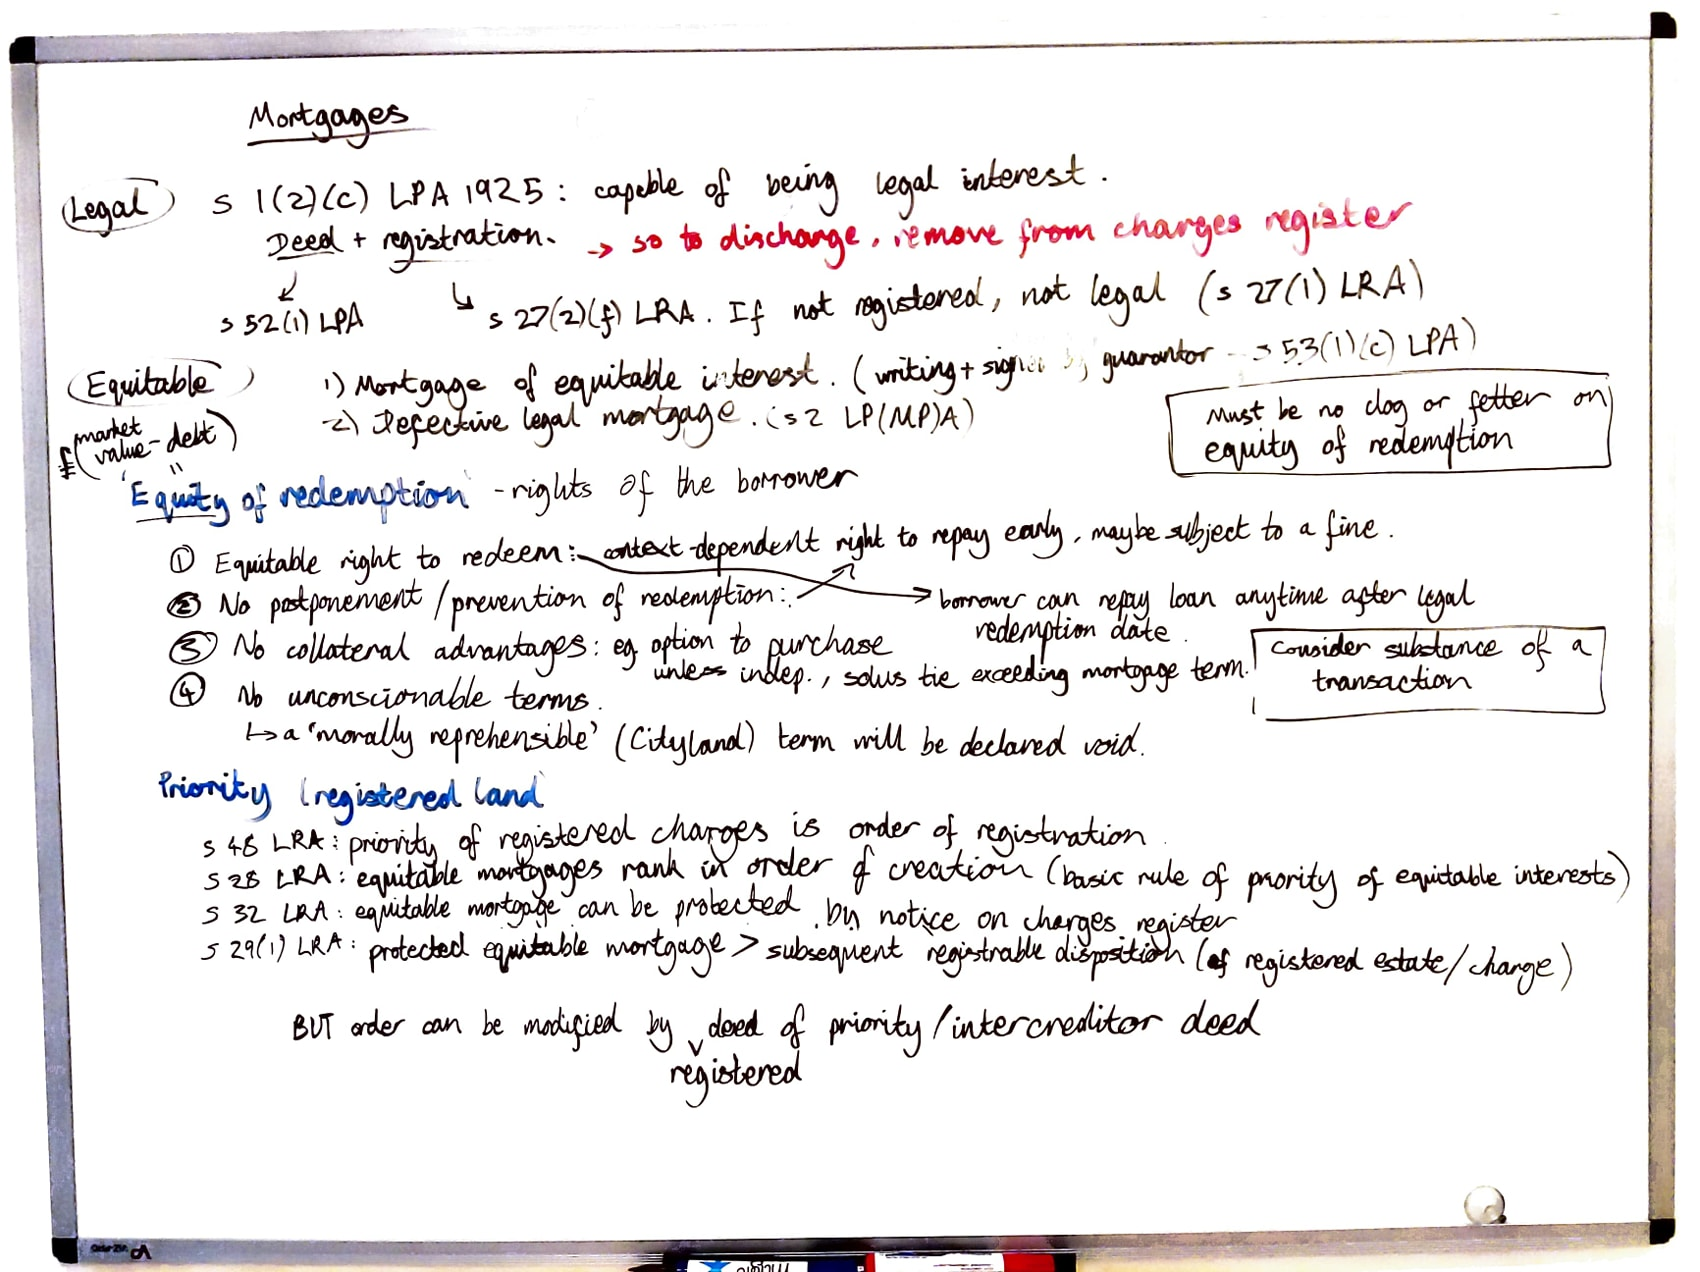
\includegraphics{C:/Users/shiva/Filen/MEGA/LegalPracticeCourse/mortgages 1_1.jpg}

\begin{env-615494ee-4c11-425d-a24a-676608cc22a4}

Definition

A mortgage is a bundle of proprietary rights granted to the lender (the
mortgagee) as security for a loan.

\end{env-615494ee-4c11-425d-a24a-676608cc22a4}

\hypertarget{legal-mortgages}{%
\subsubsection{Legal Mortgages}\label{legal-mortgages}}

Per LPA 1925, s 1(2)(c) a mortgage is capable of being a legal interest
in land. In order to be recognised as a legal interest, the mortgage
must be created in compliance with the formalities for a legal interest
over registered land. These are deed and registration.

\hypertarget{deed}{%
\paragraph{Deed}\label{deed}}

\begin{env-9843ce55-0506-497d-95ba-03a690b05b3c}

\href{https://www.legislation.gov.uk/ukpga/Geo5/15-16/20/section/52}{s
52(1) LPA 1925}

All conveyances of land or of any interest therein are void for the
purpose of conveying or creating a legal estate unless made by deed.

\end{env-9843ce55-0506-497d-95ba-03a690b05b3c}

To be valid, the deed must comply with the requirements set out in
\href{https://www.legislation.gov.uk/ukpga/1989/34/section/1}{s 1
LP(MP)A 1989}:

\begin{itemize}
\tightlist
\item
  A deed must be clear on the face of the document that it is intended
  to be a deed.
\item
  The deed must be validly executed.
\item
  The deed must be delivered.
\end{itemize}

\hypertarget{registration}{%
\paragraph{Registration}\label{registration}}

The mortgage deed must then be registered at the Land Registry
(\href{https://www.legislation.gov.uk/ukpga/2002/9/section/27}{s
27(2)(f) LRA 2002}). If it is not registered, the mortgage will not take
effect as a legal mortgage in the land (s 27(1)) but could still be an
equitable interest.

Dispositions are required to be registered:

\begin{env-9843ce55-0506-497d-95ba-03a690b05b3c}

\href{https://www.legislation.gov.uk/ukpga/2002/9/section/27}{s 27 LRA
2002}

(1) If a disposition of a registered estate or registered charge is
required to be completed by registration, it does not operate at law
until the relevant registration requirements are met.

(2) In the case of a registered estate, the following are the
dispositions which are required to be completed by
registration---\ldots{}

(f) the grant of a legal charge

\end{env-9843ce55-0506-497d-95ba-03a690b05b3c}

\hypertarget{legal-vs-equitable}{%
\subsubsection{Legal Vs Equitable}\label{legal-vs-equitable}}

If the mortgage is being granted over a legal estate by the legal owner,
the mortgage is capable of being a legal interest. Consider if the
mortgage has been granted by deed and properly registered. If it has,
the parties have created a valid legal mortgage. You do not need to
consider equitable mortgages in this scenario.

If:

\begin{enumerate}
\tightlist
\item
  the mortgagor (the borrower) only holds an equitable interest in the
  land (rather than being a legal owner), or
\item
  the mortgage is a defective legal mortgage (it does not comply with
  the requirements of a deed, or it has not been registered)
\end{enumerate}

Then consider if there is an equitable mortgage on the facts.

\hypertarget{equitable-mortgages}{%
\subsubsection{Equitable Mortgages}\label{equitable-mortgages}}

An equitable mortgage can arise for a number of reasons.

\hypertarget{mortgages-of-equitable-interests}{%
\paragraph{Mortgages of Equitable
Interests}\label{mortgages-of-equitable-interests}}

Where the borrower holds an equitable interest in the land (i.e., they
are not a legal owner, e.g., a beneficiary in a trust of land), any
mortgage of that interest will be equitable in nature. Such a mortgage
can be created very informally. In accordance with
\href{https://www.legislation.gov.uk/ukpga/Geo5/15-16/20/section/53}{s
53(1)(c) LPA 1925}, such a mortgage need only be in writing and signed
by the grantor in order to be validly created.

\hypertarget{defective-legal-mortgages}{%
\paragraph{Defective Legal Mortgages}\label{defective-legal-mortgages}}

A mortgage over registered land which is not granted by a valid deed or
that is not completed by registration will not take effect as a legal
mortgage (it will be defective). However, it may be regarded as an
equitable mortgage if it complies with
\href{https://www.legislation.gov.uk/ukpga/1989/34/section/2}{s 2
LP(MP)A 1989}. Equity will recognise it as a `contract to grant a legal
mortgage' providing it is in writing, contains all the agreed terms and
is signed by both the mortgagor and mortgagee.

\hypertarget{discharge-of-mortgages}{%
\paragraph{Discharge of Mortgages}\label{discharge-of-mortgages}}

Once a mortgage has been repaid in full, the mortgage entries at the
Land Registry must be cancelled. A mortgage is only considered to be
fully discharged when all reference to it has been removed from the
Charges Register at the Land Registry.

Discharge of a registered charge is done by using a specific Land
Registry form. A
\href{https://assets.publishing.service.gov.uk/government/uploads/system/uploads/attachment_data/file/808695/DS1__2019-06-17_.pdf}{DS1
form} is used to discharge a mortgage over the whole of the land in a
title.

If only part of the land in the title is being released from the
mortgage, for example if only part of the land is being sold to a buyer,
a
\href{https://assets.publishing.service.gov.uk/government/uploads/system/uploads/attachment_data/file/713043/DS3__2018-05-25_.pdf}{DS3
form} is used.

\hypertarget{summary}{%
\subsubsection{Summary}\label{summary}}

MERMAID2

See Equity of redemption.

\hypertarget{undue-influence}{%
\subsubsection{Undue Influence}\label{undue-influence}}

See Undue influence.

\hypertarget{context-2}{%
\paragraph{Context}\label{context-2}}

Consider a scenario where a married couple own the freehold to their
family home. A bank lends some money to the wife's business on the
condition that the bank is granted a mortgage over the property.

In the ordinary rules of priority, interests rank according to which was
created first. This means the bank's right in the land would rank behind
the husband's and wife's as the freehold owners -- their interest (i.e.,
their freehold ownership) was created before the bank's.

The mortgage deed will contain a provision stating that the bank
interest ranks in priority to the freehold ownership, which means the
bank can possess and sell if the land if the repayments stop. The effect
of this priority provision is that the Bank's interest in the land will
rank ahead of the husband and wife's interest. This happens in all
mortgage deals and means the bank and lender will be able to repossess
and then sell the land in the event of default.

Suppose the mortgage repayments stop and the bank wishes to enforce its
security over the house. The issue for the bank here is that the loan
was not for the joint benefit of both the husband and wife. If the
husband can successfully argue that he was unduly influenced into
entering the mortgage deed then the effect is that the mortgage will be
unenforceable against him (Barclays Bank plc v O'Brien {[}1994{]} 1 AC
180) because the clause which postpones his interest in favour of the
bank's is ineffective.

To ensure that the bank has priority, it must follow the guidelines set
out in RBS v Etridge (No 2) {[}2002{]} 2 AC 773.

These guidelines provide that the lender must write to the party who is
granting the mortgage not for their benefit (the husband in the example
we've looked at) explaining that the Bank needs confirmation from an
independent solicitor that he/she has explained the transaction to
him/her.

\begin{itemize}
\tightlist
\item
  The bank will ask that party to nominate an independent solicitor
\item
  Provide all information to that independent solicitor
\item
  And the bank must not proceed to lend until confirmation received from
  the independent solicitor that the transaction has been fully
  explained.
\end{itemize}

The solicitor must:

\begin{itemize}
\tightlist
\item
  Meet the party who is entering into the mortgage not for their own
  benefit face to face, on their own (i.e., not with the partner for
  whose benefit the mortgage loan is for!)
\item
  Explain why they have to come to see him/her, i.e., to stop them from
  being able to claim UI later
\item
  explain documents and transaction in a meaningful way using
  non-technical language
\item
  Point out the risks
\item
  Emphasise he/she has a choice
\item
  keep a detailed attendance note and confirm everything in writing
\item
  send certificate to Bank.
\end{itemize}

\begin{env-7ede146d-a28c-46fa-985d-64c388b7528b}

Warning

The House of Lords in Etridge said these steps should be taken in every
non-commercial case where a private individual offers his property as
security for another person's debts.

\end{env-7ede146d-a28c-46fa-985d-64c388b7528b}

\hypertarget{priority-of-mortgages-over-registered-land}{%
\subsubsection{Priority of Mortgages Over Registered
Land}\label{priority-of-mortgages-over-registered-land}}

There is an order of priority for mortgages on a piece of land.

\hypertarget{legal-mortgages-1}{%
\paragraph{Legal Mortgages}\label{legal-mortgages-1}}

Under the LRA all mortgages over registered land must themselves be
registered substantively in order to attain the status of a legal
mortgage
(\href{https://www.legislation.gov.uk/ukpga/2002/9/section/27}{LRA 2002,
s 27(2)(f)}).

Once registered, they take effect as a `registered charge' under the
LRA.

A mortgage over registered land which is not completed by substantive
registration will not take effect as a legal mortgage
(\href{https://www.legislation.gov.uk/ukpga/2002/9/section/27}{s 27(1)
LRA 2002}).

Under \href{https://www.legislation.gov.uk/ukpga/2002/9/section/48}{LRA
2002, s 48} priority between registered charges depends upon the order
in which they are entered on the register. This is regardless of the
order of creation. Where two or more mortgages are created at the same
time (i.e., first and second mortgage simultaneously), the application
for registration will specify the order of priority.

Priority between registered charges depends upon the order in which they
are registered.

\hypertarget{equitable-mortgages-1}{%
\paragraph{Equitable Mortgages}\label{equitable-mortgages-1}}

An equitable mortgage can arise for a number of reasons. The two most
common are:

\begin{itemize}
\tightlist
\item
  Mortgages of equitable interests
\item
  Defective legal mortgages.
\end{itemize}

\hypertarget{basic-rule}{%
\subparagraph{Basic Rule}\label{basic-rule}}

As against another equitable mortgagee, equitable mortgages rank in
order of creation
(\href{https://www.legislation.gov.uk/ukpga/2002/9/section/28}{LRA 2002,
s 28}). This is the `basic rule' of priority that applies to all
equitable interests because an equitable interest in the land can be
validly created and exist without registration.

\hypertarget{protected-equitable-mortgage}{%
\subparagraph{Protected Equitable
Mortgage}\label{protected-equitable-mortgage}}

Although not required in order to validly create it, an equitable
mortgage over registered land can be protected by the entering of a
notice on the charges register
(\href{https://www.legislation.gov.uk/ukpga/2002/9/section/32}{LRA 2002,
s 32}).

If protected by the entry of a notice, an equitable mortgage over
registered land will take \textbf{priority} over a subsequent legal
mortgage,
\href{https://www.legislation.gov.uk/ukpga/2002/9/section/29}{LRA 2002,
s 29(1)}. As between competing equitable mortgages, this \textbf{does
not} affect the priority, which will always be determined by creation.

However, an equitable mortgage not protected by a notice, will not take
priority (i.e., lose its priority) to a subsequent registrable
disposition of either a registered estate or a registered charge
(\href{https://www.legislation.gov.uk/ukpga/2002/9/section/29}{LRA 2002,
s 29(1)}). (i.e., a transfer of the legal estate for value or the grant
of a legal mortgage)

\begin{env-de3101d4-f08b-48eb-bc0e-2fa06f3bcf8e}

Example

A borrower grants a mortgage to Lender A. Although the mortgage is
granted by a valid deed, Lender A fails to register the mortgage at the
Land Registry -- it is a \textbf{defective legal mortgage}. However,
because it is in writing, signed by both the borrower and Lender A and
contains the agreed mortgage term, the mortgages take effect an
\textbf{equitable mortgage}.

The borrower subsequently enters into a second mortgage with Lender B.
The mortgage is granted by valid deed, which Lender B registers. The
mortgage therefore takes effect as \textbf{a valid legal mortgage}.

As a \textbf{registrable disposition of a legal charge over a registered
estate}, the legal mortgage in favour of Lender B will rank ahead of the
equitable mortgage in favour of Lender A.

The borrower then enters into a further mortgage with Lender C. Although
the borrower and Lender C enter into a document labelled as a deed, the
borrower's signature is not witnessed. There is no valid execution and
the \textbf{legal mortgage is defective}. As the document is in writing,
contains all the agreed terms and is signed by the borrower and Lender
C, there is an \textbf{equitable mortgage}, which Lender C proceeds to
\textbf{note on the charges register} of the borrower's registered
title.

If the borrower defaults in their mortgage repayments and the land has
to be sold, who then gets paid first? Which mortgage ranks in priority?

Lender A has an equitable mortgage which was created first, but not
protected. Lender B has a legal mortgage. Lender C has an equitable
mortgage which has been duly protected.

Lender B will get paid first. It take priority of Lender A's equitable
mortgage because the equitable mortgage was not protected by notice at
the Land Registry.

Lender A will then get paid second because Lender A and C both have
equitable mortgages and as between competing equitable mortgages, the
order of creation determines priority.

The fact Lender C protected its equitable mortgage by the entry of a
notice, does not affect priority here. However, if a subsequent legal
mortgage were entered into by the borrower, Lender C would take priority
over this because it has protected its interest.

\end{env-de3101d4-f08b-48eb-bc0e-2fa06f3bcf8e}

\hypertarget{postponement}{%
\subparagraph{Postponement}\label{postponement}}

The priority rules discussed can be modified to allow a mortgage to take
priority over a pre-existing interest which could otherwise enjoy
priority if there is a postponement of that pre-existing interest.
Lenders can agree to alter the position that would apply according to
the priority rules by entering into a \textbf{deed of priority} or
\textbf{intercreditor deed}.

Any agreement would need to be \textbf{registered} at the Land Registry.

\begin{env-99436a7e-0b1e-438d-960f-947d510b2b61}

Important

Mortgagees will also often require an express waiver or postponement to
be included in a mortgage agreement so that the rights of any person
living at the mortgaged property with the mortgagor are postponed to the
interests of the mortgagee.

This is important for the lender to be able to enforce their security
and take possession of the mortgaged property in the event of default.

If the lender's interest in the land does not rank in priority to the
interest of a person in occupation (not a party to the mortgage) then
the lender would not be able to take possession of the land in order to
exercise its power of sale.

\end{env-99436a7e-0b1e-438d-960f-947d510b2b61}

\hypertarget{rights-of-the-lender}{%
\subsubsection{Rights of the Lender}\label{rights-of-the-lender}}

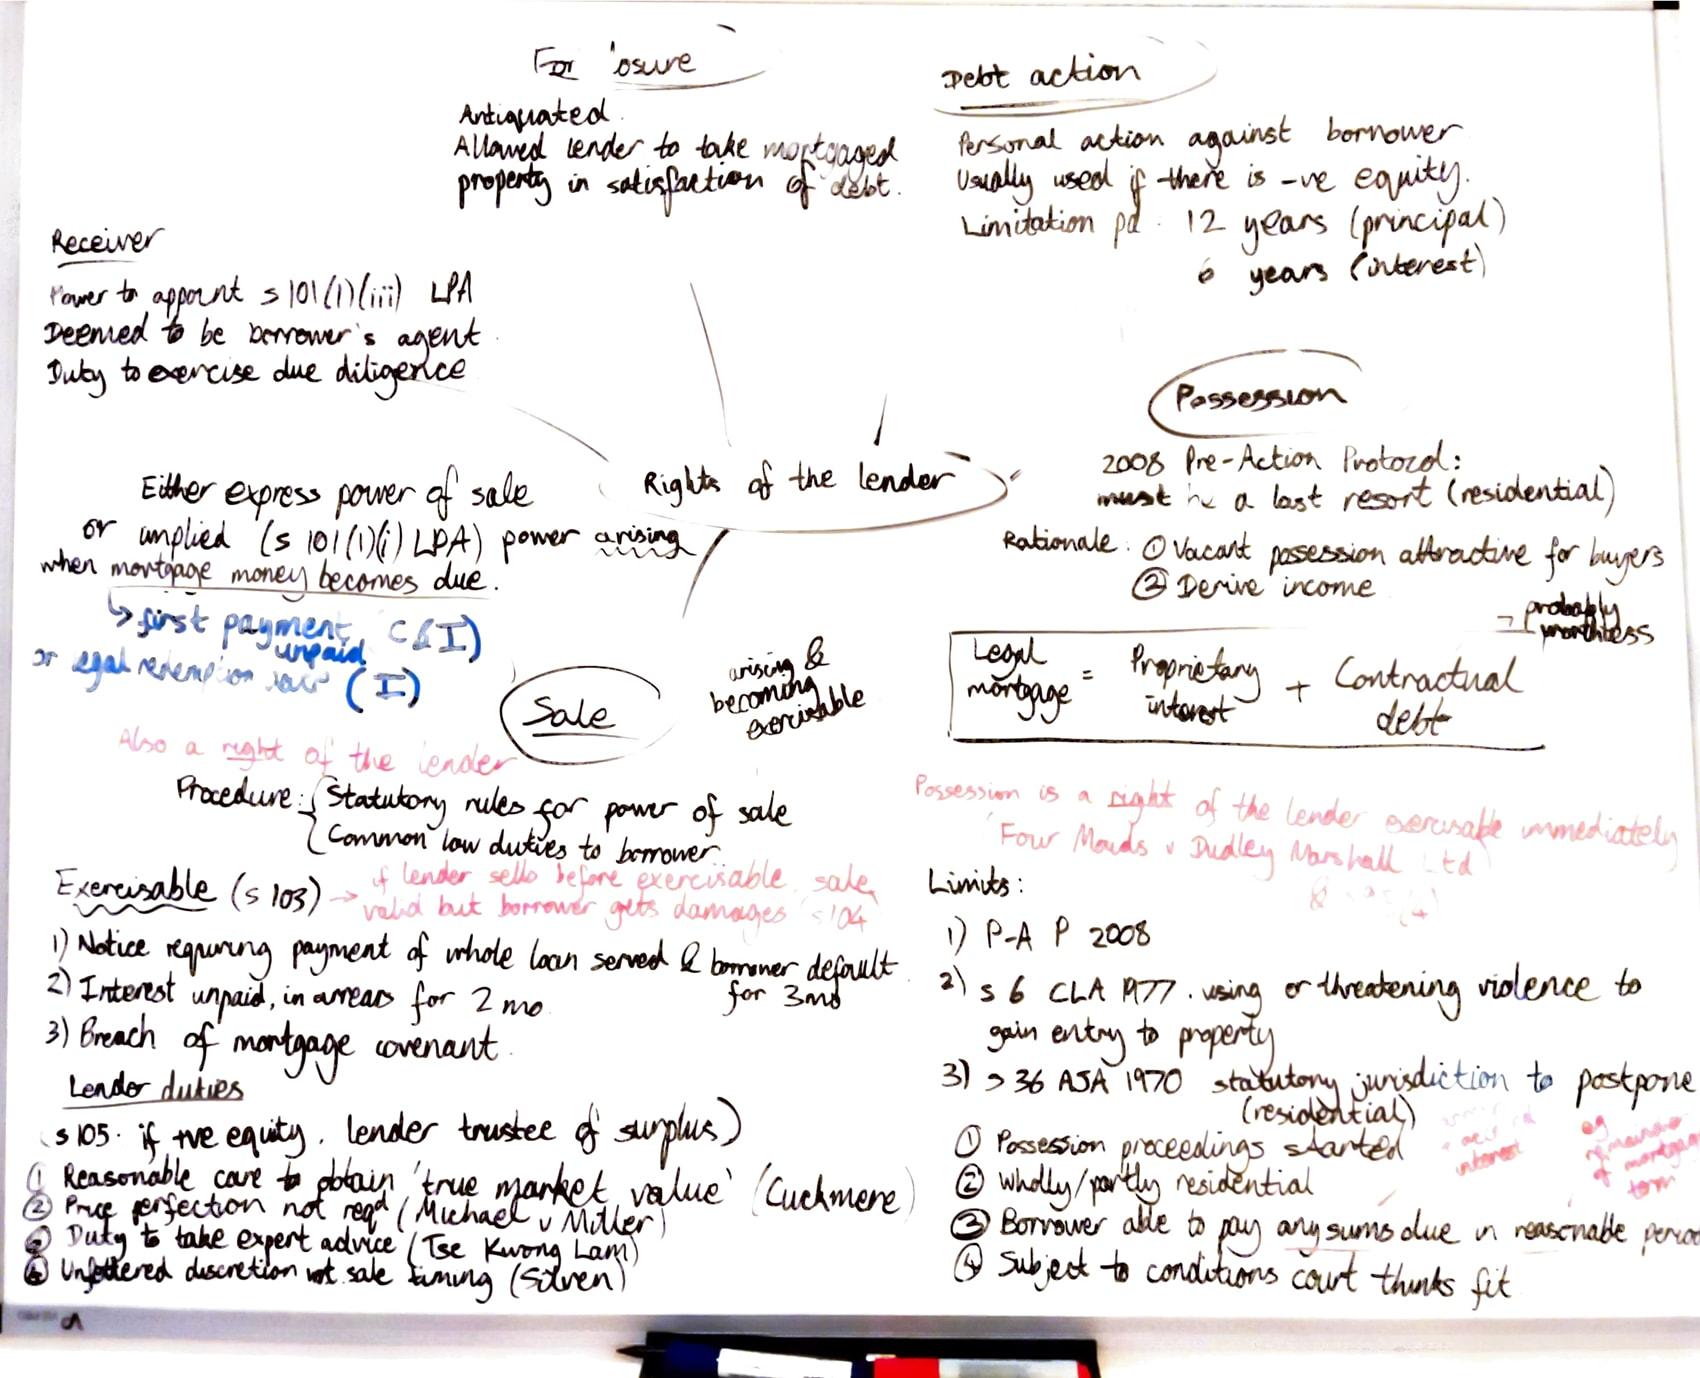
\includegraphics{C:/Users/shiva/Filen/MEGA/LegalPracticeCourse/rights of a lender_1.jpg}

It is inherent in the nature of a mortgage that the lender's right to
repayment of the loan is secured against the mortgaged property itself.
This security is very important to lenders, as without it, they may take
the view that it is simply too much of a risk to advance large sums of
money to borrowers.

If the mortgagor fails to make the mortgage payments, the lender will
wish to take steps to protect itself against losses. The lender can
always sue the borrower in contract for the debt, but this can be a long
and ultimately fruitless process if the borrower has insufficient money.
The fact that a mortgage is a proprietary right in the lender's favour
means that the lender has several remedies available to it. These
remedies are:

\begin{itemize}
\tightlist
\item
  Debt action
\item
  Possession
\item
  Sale
\item
  Receiver
\item
  Foreclosure.
\end{itemize}

There is no obligation for a lender to exercise any particular remedy,
or indeed any remedy at all. The choice of remedy is a matter for the
particular lender in the particular circumstances. However, if the
lender does decide to pursue a remedy, it will be under a duty to act
fairly and reasonably, and may be subject to additional duties to the
borrower, depending on the remedy sought.

The lender who holds the security of a legal mortgage, rather than an
equitable one, has a wider choice of remedies than an equitable
mortgagee.

An equitable mortgagee has the same rights to bring a debt action under
the mortgage contract for money owed, to apply for foreclosure, and to
appoint a receiver. However, the equitable lender does not, generally
speaking, have the right to repossess or sell without a court order.

\hypertarget{debt-action}{%
\paragraph{Debt Action}\label{debt-action}}

The contractual debt action is a personal action against the borrower.
As the lender has a proprietary right and can enforce it against the
property itself, it may be thought that the contractual right to sue for
the outstanding debt is rarely used. In fact, it is used in addition to,
not instead of, one of the other remedies, and in recent years, has been
used in particular situations.

If the value of the mortgaged property is less than the outstanding
mortgage debt, there is said to be \textbf{negative equity}. The lender
may take possession of and sell the property, but if the sale proceeds
so not cover the outstanding debt, the lender will wish to pursue a
personal debt action against the borrower for the shortfall.

The limitation period for a contractual debt is not straightforward: if
the mortgage has been created by deed, as all legal mortgages must be,
then the period for recovery of the debt stated in the deed (the
capital) is \textbf{twelve years}. The limitation period for recovery of
interest is \textbf{six years}. What this means in reality is that
borrowers can find themselves involved in contractual debt actions many
years after repossession, when they may have thought that their troubles
were behind them.

\hypertarget{possession}{%
\paragraph{Possession}\label{possession}}

A legal lender may wish to enforce its security by taking possession of
the mortgaged property as a precursor to sale. There are two reasons a
lender may wish to do this:

\begin{itemize}
\tightlist
\item
  Possession will enable the lender to offer the property for sale with
  vacant possession, free from any rights of the borrower. Vacant
  possession makes a property more attractive to a potential buyer and
  will enable a higher price to be obtained.
\item
  Possession will enable the lender to manage the property and derive an
  income from it. The income can then be used to reduce the outstanding
  mortgage debt.
\end{itemize}

Since 2008, the \textbf{Pre-Action Protocol} in residential cases,
possession must be a last resort. The mortgage lender is expected to
explore alternative arrangements with the borrower, such as extending
the mortgage term and/or scheduling a new payment plan.

\hypertarget{sale}{%
\paragraph{Sale}\label{sale}}

The power of sale is the strongest right which the lender can use
against a defaulting borrower. If exercised, the borrower loses all
rights to the property. The sale proceeds are applied towards the
outstanding debt. If there is a surplus, this will be forwarded to the
borrower; but if there is a shortfall, the borrower may be sued
personally by the lender for the outstanding contractual debt.

Because the power of sale has such drastic consequences for the
borrower, there are procedural steps which must be adhered to:

\begin{itemize}
\tightlist
\item
  The power of sale must have arisen in accordance with statutory rules;
\item
  The power of sale must be exercisable in accordance with statutory
  rules; and
\item
  The lender must fulfil its duties on sale, which have largely arisen
  from case law.
\end{itemize}

\hypertarget{receiver}{%
\paragraph{Receiver}\label{receiver}}

A receiver acts as manager of the mortgaged property if the lender does
not wish to take possession or to sell. The power to appoint a receiver
arises under
\href{https://www.legislation.gov.uk/ukpga/Geo5/15-16/20/section/101}{LPA
1925, s 101(1)(iii)}. The receiver is an administrator whose function is
to get an income from the land, for example by continuing an existing
business, and will apply it towards the outstanding mortgage debt.

The receiver is deemed to be the borrower's agent. This may seem odd, as
the receiver is appointed by the lender, but it means that the lender is
not liable for the receiver's negligence. Thus, the appointment of a
receiver is a safer option for the lender than taking possession and
running the business itself.

A receiver must act with due diligence, subject always to the main duty
of paying off the mortgage debt (Medforth v Blake {[}2000{]} Ch 86).

\hypertarget{foreclosure}{%
\paragraph{Foreclosure}\label{foreclosure}}

Foreclosure is a historic way of enforcing a mortgage which is rarely
used nowadays. It allows a lender to take the mortgaged property in
satisfaction of the debt, meaning that the freehold will vest in the
lender, and the borrower will lose all rights to the property. This
could happen even though there may be only a very small amount
outstanding on the mortgage security, when compared to the value of the
property as a whole.

From the lender's point of view, the procedure is lengthy and complex.
The court may order a sale in lieu of foreclosure, and almost certainly
will do so if the property is worth a lot more than the outstanding
debt. Even after the final decree of foreclosure, the borrower can
re-open the case if he can show that he has the means to pay.

From the borrower's point of view, there are some advantages in that an
order of foreclosure extinguishes all other mortgages secured on the
property. It also extinguishes the mortgagor's contractual debt, so the
lender cannot pursue the borrower for any surplus debt over and above
the value of the property.

Today, foreclosure is viewed as a particularly Draconian remedy and is
rarely encountered in practice. The Law Commission has recommended that
it be abolished and replaced by wider powers for the lender to sell the
property.

\hypertarget{lenders-right-to-possess}{%
\subsubsection{Lender's Right to
Possess}\label{lenders-right-to-possess}}

\hypertarget{legal-mortgage}{%
\paragraph{Legal Mortgage}\label{legal-mortgage}}

A legal mortgage comprises both a proprietary interest and a contractual
debt. If the borrower defaults, it is unlikely that a debt action will
be worthwhile. The lender will therefore wish to enforce its security by
selling the property and recovering the outstanding debt from the sale
proceeds. The Lender will need to repossess the mortgaged property in
order to sell `with vacant possession' and acquire the best possible
price. The lender may also require possession in order to manage the
property and generate an income to pay the outstanding mortgage debt.

\href{https://www.legislation.gov.uk/ukpga/Geo5/15-16/20/section/95}{LPA
1925, s 95(4)} acknowledges `the right of a mortgagee of land\ldots{} to
take possession', and in Four Maids v Dudley Marshall (Properties) Ltd
{[}1957{]} Ch 317 it was confirmed that the right arises as soon as the
mortgage is granted, `before the ink\ldots{} becomes dry' on the
mortgage deed. Possession is thus strictly a \textbf{right} of the
lender, and \textbf{not simply a remedy}. Having said that, lenders do
not exercise the right arbitrarily. It is a last resort, used when the
borrower is in default with little hope of repayment. Mortgage deeds
almost always contain a term which recognises that the right to possess
is postponed for as long as the borrower pays the agreed instalments.

\hypertarget{exercising-right-of-possession}{%
\paragraph{Exercising Right of
Possession}\label{exercising-right-of-possession}}

The right to possess is exactly what it says: a right. It is not
therefore strictly necessary for the lender to obtain a court order
prior to taking possession.

However, a series of safeguards for the borrower has evolved through
statute and case law, modifying the strict rule that a lender has a
right to possess mortgaged land even if the borrower is not in arrears
with payments.

Most of the protections are relevant for residential mortgages only.
However, all lenders have general duties to borrowers and the
\href{https://www.legislation.gov.uk/ukpga/1977/45/section/6}{Criminal
Law Act 1977, s 6} applies to all mortgage lenders.

\hypertarget{s-6-cla-1977}{%
\subparagraph{S 6 CLA 1977}\label{s-6-cla-1977}}

\href{https://www.legislation.gov.uk/ukpga/1977/45/section/6}{Criminal
Law Act 1977, s 6} makes it a criminal offence to use or threaten
violence for the purpose of gaining entry to property. This means that
exercising the right to repossess by `self-help' is risky, unless the
lender is certain that the property is unoccupied at the time.

A prudent lender will make an application to the court for an order for
possession, even though this may not be strictly necessary.

\hypertarget{pre-action-protocol-2008}{%
\subparagraph{Pre-Action Protocol 2008}\label{pre-action-protocol-2008}}

The
\href{https://www.justice.gov.uk/courts/procedure-rules/civil/protocol/prot_mha}{Pre-Action
Protocol for Possession Claims 2008} sets out the steps which a court
will expect a lender to have taken before resorting to possession of
residential property, which should be a last resort. Lenders should try
to discuss the debt with the borrower and accept reasonable requests for
a new payment plan.

Most lenders observe the Protocol. However, if they do not, they can
suffer delays in obtaining possession and may be ordered to pay the
borrower's legal costs. Non-compliance of itself does not mean that
possession is denied.

Statutory Jurisdiction to Postpone

\begin{env-9843ce55-0506-497d-95ba-03a690b05b3c}

\href{https://www.legislation.gov.uk/ukpga/1970/31/section/36}{Administration
of Justice Act (AJA) 1970, s 36}

(1) Where the mortgagee under a mortgage of land which consists of or
includes a dwelling-house brings an action in which he claims possession
of the mortgaged property, not being an action for foreclosure in which
a claim for possession of the mortgaged property is also made, the court
may exercise any of the powers conferred on it by subsection (2) below
if it appears to the court that in the event of its exercising the power
the mortgagor is likely to be able within a reasonable period to pay any
sums due under the mortgage or to remedy a default consisting of a
breach of any other obligation arising under or by virtue of the
mortgage.

(2) The court---

(a) may adjourn the proceedings, or

(b) on giving judgment, or making an order, for delivery of possession
of the mortgaged property, or at any time before the execution of such
judgment or order, may---

\begin{itemize}
\tightlist
\item
  (i) stay or suspend execution of the judgment or order, or
\item
  (ii) postpone the date for delivery of possession,
\end{itemize}

for such period or periods as the court thinks reasonable.

(3) Any such adjournment, stay, suspension or postponement as is
referred to in subsection (2) above may be made subject to such
conditions with regard to payment by the mortgagor of any sum secured by
the mortgage or the remedying of any default as the court thinks fit.

\end{env-9843ce55-0506-497d-95ba-03a690b05b3c}

The section does not:

\begin{itemize}
\tightlist
\item
  enable the court to prevent the lender from exercising its right to
  possess altogether; nor
\item
  enable the court to postpone possession in cases where there has been
  no application for an order for possession: Ropaigelach v Barclays
  Bank plc {[}2000{]} QB 263; nor
\item
  enable the court to prevent a lender from exercising a power of sale
  without first obtaining a court order: Horsham Properties Group Ltd v
  Clark {[}2009{]} 1 WLR 1255.
\end{itemize}

The section does apply where the property is wholly or partly
residential, although need not be the borrower's home. It enables the
court to adjourn possession proceedings or stay or postpone execution of
the possession order. In order to be able to do this, it must appear to
the court that the borrower is likely to be able to pay any sums due (or
remedy any other default) within a reasonable period.

\begin{env-d6ce83a0-f7a8-46b6-be95-b1235f1feb63}

Summary

\begin{itemize}
\tightlist
\item
  Possession proceedings must have started
\item
  The mortgaged property must be fully or partly residential
\item
  Borrower must be able to pay `any sums due'

  \begin{itemize}
  \tightlist
  \item
    `any sums due' means the arrears and accrued interest, and not the
    whole of the mortgage debt.
  \end{itemize}
\item
  `within a reasonable period'

  \begin{itemize}
  \tightlist
  \item
    In Cheltenham \& Gloucester Building Society v Norgan {[}1996{]} 1
    All E.R. 449 the Court of Appeal said that the starting point for
    pinpointing a `reasonable period' was the remainder of the mortgage
    term.
  \end{itemize}
\item
  Subject to such conditions `as the court thinks fit'
\end{itemize}

\end{env-d6ce83a0-f7a8-46b6-be95-b1235f1feb63}

More cases:

\begin{longtable}[]{@{}ll@{}}
\toprule()
Case & Ratio \\
\midrule()
\endhead
National \& Provincial Building Society v Lloyd {[}1996{]} 1 All ER 630
& A borrower requesting a postponement of possession should present a
detailed financial plan to the court, showing how the loan and arrears
will be paid off before the term expires. \\
Bristol and West Building Society v Ellis (1997) 73 P\&CR 158 & A
postponement was granted to allow the borrowers to achieve a sale of the
property themselves. The court needed to see that the sale proceeds
would be sufficient to cover the debt due. An estate agent's optimistic
estimate of the price likely to be achieved would not be enough. \\
Mortgage Services Funding plc v Steele (1996) 72 P\&CR 40 & In order to
grant a postponement to allow the borrower to sell, the court required
firm evidence of an imminent exchange of contracts. Simply instructing a
solicitor to handle the conveyancing will not be enough: courts are
suspicious of mortgagor's delaying tactics, enabling them to stay in
possession for longer. \\
Target Home Loans Ltd v Clothier {[}1994{]} 1 All ER 439 & The court
awarded a short, three-month postponement of possession to allow the
borrower to sell the property. There was evidence from an estate agent
that a genuine offer had been received. \\
\bottomrule()
\end{longtable}

\hypertarget{lenders-right-to-sell-and-duties}{%
\subsubsection{Lender's Right to Sell and
Duties}\label{lenders-right-to-sell-and-duties}}

The right to sell is the strongest of the lender's rights and there are
strict rules as to when the power arises and when it becomes
exercisable. As this power of sale is a right of the lender, no court
order is required. The power of sale must exist, have arisen and become
exercisable.

The lender's statutory power of sale which arises under the Law of
Property Act 1925 is explored. If there are co-owners of the property
who are not a party to the mortgage, the lender will instead rely on the
provisions of the
\href{https://www.legislation.gov.uk/ukpga/1996/47/contents}{Trusts of
Land and Appointment of Trustees Act 1996}.

\hypertarget{when-is-there-a-right-to-sell}{%
\paragraph{When is There a Right to
Sell}\label{when-is-there-a-right-to-sell}}

\hypertarget{express-power-of-sale}{%
\subparagraph{Express Power of Sale}\label{express-power-of-sale}}

Most mortgage documents will include an express power of sale and will
set out exactly how and when the power will be exercised. The lender
will not need to rely on \textbf{any} statutory provisions, although it
will be subject to duties on sale, in the same was as a lender relying
on statutory powers.

\hypertarget{implied-power-of-sale}{%
\subparagraph{Implied Power of Sale}\label{implied-power-of-sale}}

In the absence of an express power, a right to sell can be implied under
\href{https://www.legislation.gov.uk/ukpga/Geo5/15-16/20/section/101}{LPA
1925, s 101(1)(i)} unless it is excluded or modified in the mortgage
deed.

\begin{env-9843ce55-0506-497d-95ba-03a690b05b3c}

\href{https://www.legislation.gov.uk/ukpga/Geo5/15-16/20/section/101}{LPA
1925, s 101(1)(i)}

(1) A mortgagee, where the mortgage is made by deed, shall, by virtue of
this Act, have the following powers, to the like extent as if they had
been in terms conferred by the mortgage deed, but not further (namely):

(i) A power, \textbf{when the mortgage money has become due}, to sell,
or to concur with any other person in selling, the mortgaged property,
or any part thereof, either subject to prior charges or not, and
\textbf{either together or in lots, by public auction or by private
contract}, subject to such conditions respecting title, or evidence of
title, or other matter, as the mortgagee thinks fit, with power to vary
any contract for sale, and to buy in at an auction, or to rescind any
contract for sale, and to re-sell, without being answerable for any loss
occasioned thereby;

\end{env-9843ce55-0506-497d-95ba-03a690b05b3c}

\hypertarget{when-does-the-right-arise}{%
\subparagraph{When Does the Right
Arise?}\label{when-does-the-right-arise}}

The lender's statutory power of sale arises `when the mortgage money has
become due':

\begin{itemize}
\tightlist
\item
  If a borrower has a capital and interest repayment mortgage Payne v
  Cardiff {[}1932{]} 1 KB 241 confirms that the power of sale arises as
  soon as one portion of capital is due, meaning that it arises as soon
  as one payment is unpaid.
\item
  Where a mortgage is an interest-only mortgage, the capital is not due
  until the end of the loan term. In these cases, the mortgage money
  will `become due' at the \textbf{legal redemption date}, usually about
  six months from the start of the mortgage.
\end{itemize}

If the lender sells after the power has arisen but before it is
exercisable, a sale to an innocent purchaser will be valid, but the
lender will be liable in damages to the
borrower,\href{https://www.legislation.gov.uk/ukpga/Geo5/15-16/20/section/104}{LPA
1925, s 104}.

\hypertarget{when-is-the-right-exercisable}{%
\subparagraph{When is the Right
Exercisable?}\label{when-is-the-right-exercisable}}

Where the right to sell has been expressly conferred, the wording will
set out in what circumstances the power can be exercised.

If the power arises under
\href{https://www.legislation.gov.uk/ukpga/Geo5/15-16/20/section/101}{LPA
1925, s 101(1)(i)}, the power will become exercisable only when at least
one of the criteria in
\href{https://www.legislation.gov.uk/ukpga/Geo5/15-16/20/section/103}{s
103 LPA 1925} applies:

\begin{enumerate}
\tightlist
\item
  Notice requiring payment of the whole loan has been served by the
  lender and the borrower has defaulted -- No arrears are necessary
  here: the lender can request the full loan at any time.
\item
  Interest is unpaid and arrears for at least two months. This does not
  mean that two months' interest must be owed: there must be some
  interest outstanding for two months: it does not need to be a large
  sum!
\item
  There has been some breach of another mortgage provision, such as a
  covenant to keep the mortgaged property insured or in good repair.
  Examples: failure to insure the property or allowing it to fall into
  disrepair: basically something which could affect the value of the
  security.
\end{enumerate}

\hypertarget{lenders-duties-when-selling}{%
\subparagraph{Lender's Duties When
Selling}\label{lenders-duties-when-selling}}

When the lender exercises its right to sell mortgaged property, whether
the right is conferred expressly or by statute, it owes duties to the
borrower. The lender's basic motive is to recover the debt due, meaning
the capital sum, interest and costs. It is not necessarily interested in
achieving the best possible price. The cases show that the lender cannot
simply consider its own interests: these must be balanced against the
interests of the borrower.

After the sale, the lender is trustee of the surplus proceeds of the
sale
\href{https://www.legislation.gov.uk/ukpga/Geo5/15-16/20/section/105}{(LPA
1925, s 105}) and must hand them to the person next entitled. That may
be another lender, or the borrower.

\begin{longtable}[]{@{}ll@{}}
\toprule()
Case & Ratio \\
\midrule()
\endhead
Cuckmere Brick Co Ltd v Mutual Finance Ltd {[}1971{]} Ch 949 & The
lender owed the borrower a duty to take reasonable care to obtain the
`true market value' or `proper price' for the property. \\
Michael v Miller {[}2004{]} EWCA Civ 282 & Perfection as to price is not
required: the lender will not be liable for losses if the price is
within the correct bracket or within an acceptable `margin of error'. \\
Tse Kwong Lam v Wong Chit Sen {[}1983{]} 1 WLR 1349 & A lender cannot
simply put the property `under the hammer' as a matter of course.
Lenders are under a duty to take expert advice as to the method of sale,
the marketing strategy and the reserve price. \\
Silven Properties Ltd v Royal Bank of Scotland plc {[}2004{]} 4 All ER
484 & A lender has an `unfettered discretion' as to when to sell and can
not be expected to delay in order to improve the property or wait for an
upturn in the property market. \\
\bottomrule()
\end{longtable}

See also Scott v Southern Pacific Mortgages Limited {[}2014{]} UKSC 52.

\begin{itemize}
\tightlist
\item
  Or 'charge by way of legal mortgage'
\item
  Security for loan created by deed
\item
  If completed by registration, will be binding on successors in title
\item
  Remove from title on completion.
\end{itemize}

\hypertarget{co-ownership}{%
\subsection{Co-ownership}\label{co-ownership}}

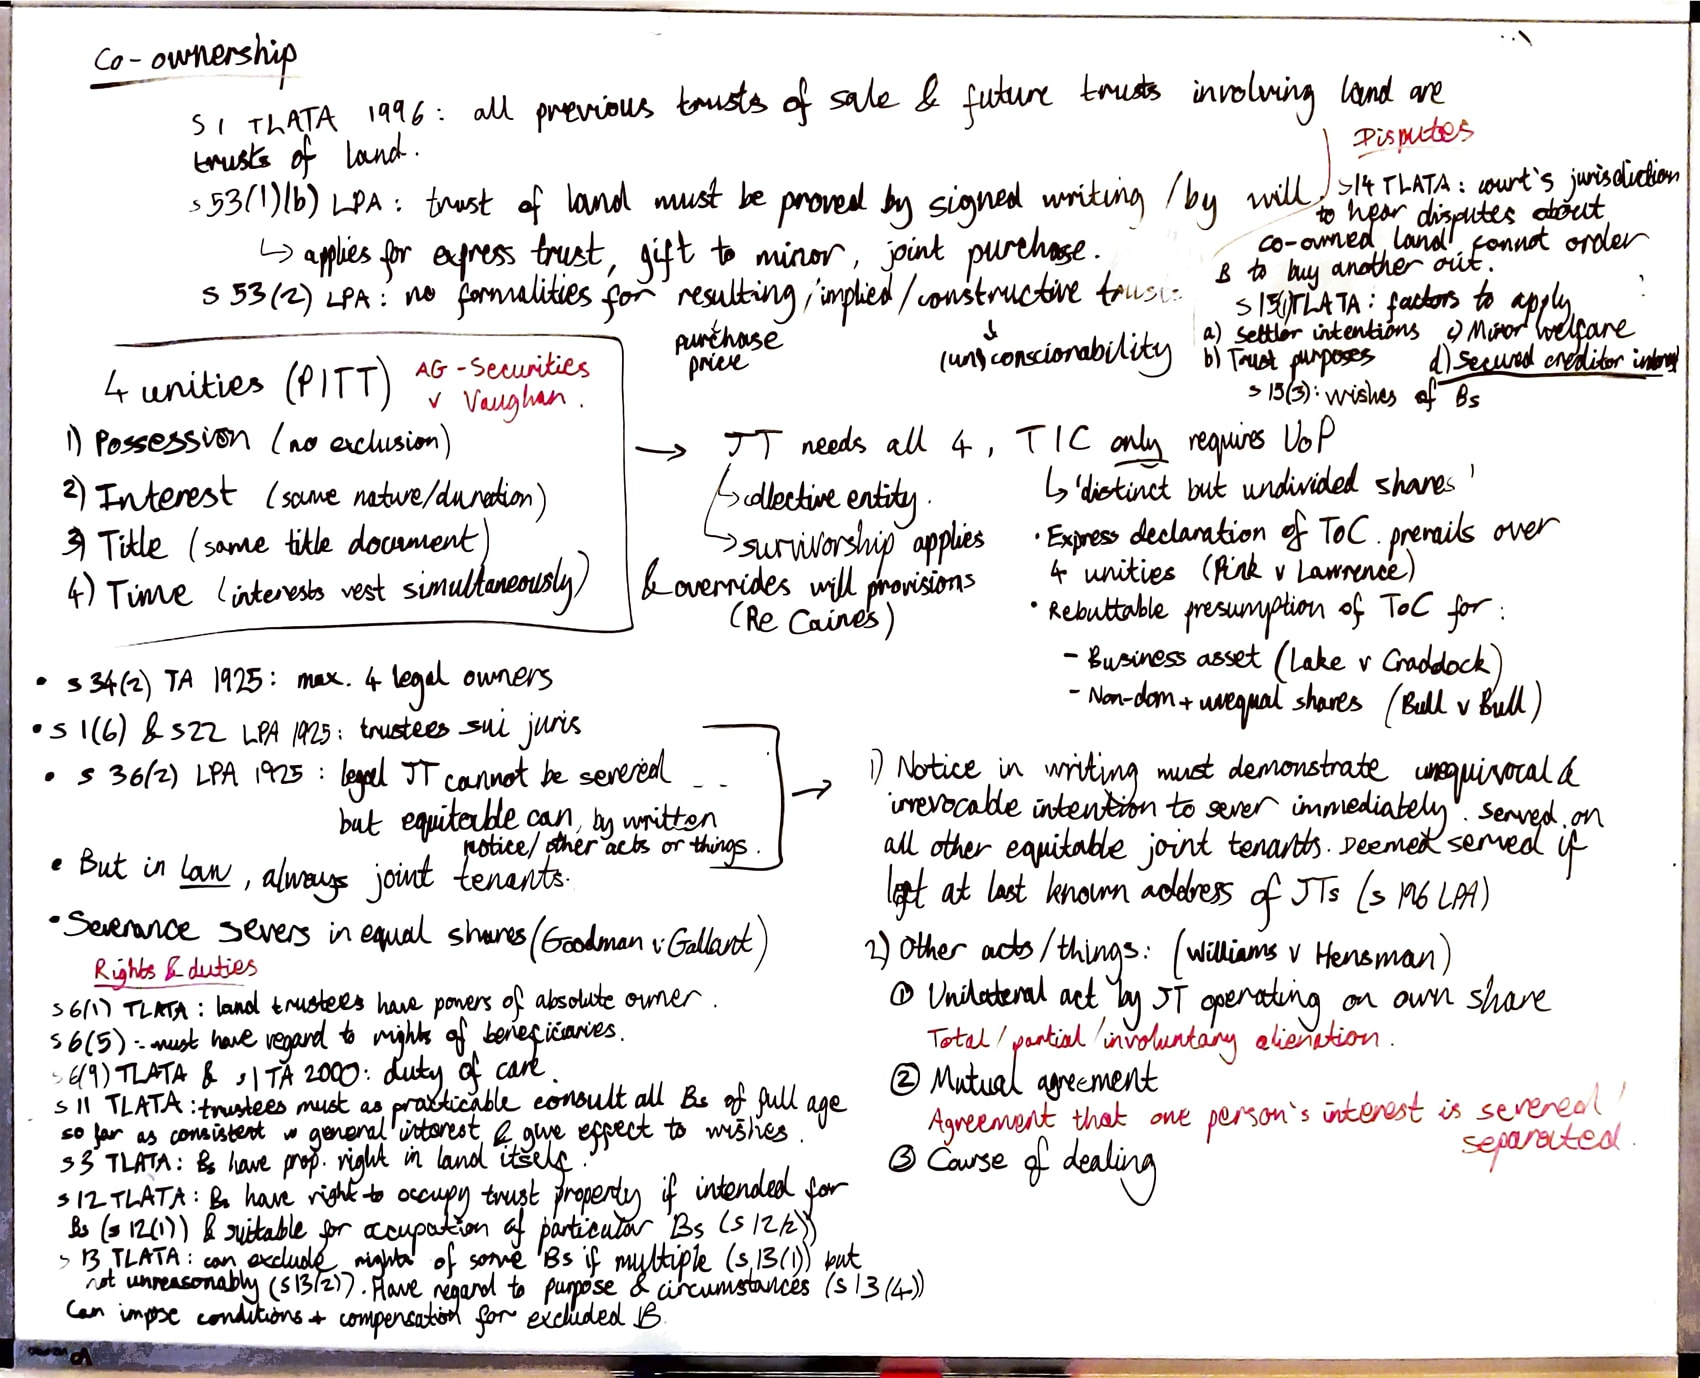
\includegraphics{C:/Users/shiva/Filen/MEGA/LegalPracticeCourse/Co-Ownership_1.jpg}

\hypertarget{introduction-2}{%
\subsubsection{Introduction}\label{introduction-2}}

Concurrent co-ownership arises where two or more people together own the
same estate in the same piece of land at the same time. Where a couple
buys a house together, both people share the ownership of the freehold
and are said to own the freehold concurrently.

Prior to 1925, concurrent co-ownership was relatively uncommon. Most
families lived in residential accommodation held on short-term
tenancies; and if the family home was owned outright, it would generally
be owned by the husband or father.

With increased prosperity throughout the 20th century, and as the status
of women changed, it was increasingly common for husbands and wives to
own their homes jointly. Today, development has continued, with
unmarried and same-sex couples jointly purchasing their own homes.

Co-ownership is all about the legal relationship between co-owners of
land.

\hypertarget{imposition-of-a-trust}{%
\paragraph{Imposition of a Trust}\label{imposition-of-a-trust}}

Today, whenever land is owned jointly, a trust of land is imposed. This
has the effect of separating the legal title to the land, which is held
by trustees, from the equitable title, which is held by the
beneficiaries.

Ownership of the legal title does not confer any rights of enjoyment
over the land. Instead, it carries with it powers and duties of
management. The people who benefit from the trust are the beneficiaries.

It is important to understand the historical reasons for imposing a
trust, as it explains the rationale behind today's law.

The distinction between legal and equitable title can be summarised as
follows:

\begin{longtable}[]{@{}ll@{}}
\toprule()
Legal title & Equitable title \\
\midrule()
\endhead
Held by trustees & Held by beneficiaries \\
Owner(s) registered at Land Registry & Names kept private and
arrangements relating to equitable title do not appear on the
registers \\
Powers and duties of management & Enjoyment over the land. \\
\bottomrule()
\end{longtable}

\hypertarget{historical-background}{%
\paragraph{Historical Background}\label{historical-background}}

Historically,
under\href{https://www.legislation.gov.uk/ukpga/Geo5/15-16/20/section/34}{Law
of Property Act 1925, s 34(2)} and
\href{https://www.legislation.gov.uk/ukpga/Geo5/15-16/20/section/36}{s
36}, the trust which was automatically imposed when property was jointly
owned was a trust for sale. The purpose of this was to reflect attitudes
to land ownership. Land was a commodity to be invested in, in the same
way as happened with wheat, oil, and coal. Ownership was designed to
provide an income for the family. If a better investment became
available, it was imperative that the existing investment in land could
be readily sold and the proceeds invested elsewhere. To enable this to
happen, land was transferred to trustees who had a primary duty to sell
the land, and reinvest the proceeds, although they did have a power to
postpone sale.

As attitudes towards land ownership changed, and property was bought as
a long-term home rather than a short-term investment, trustees
inevitably exercised their power to postpone sale more and more often,
and for an indefinite period. This meant that the law was out of step
with society's attitudes which viewed land, and particularly the home,
as an asset to keep. The
\href{https://www.legislation.gov.uk/ukpga/1996/47/contents}{Trusts of
Land and Appointment of Trustees Act 1996} came into effect on 1 January
1997 and reformed the law. Under
\href{https://www.legislation.gov.uk/ukpga/1996/47/section/1}{s 1}, all
previous trusts for sale and all future trusts involving land are trusts
of land; and the statute governs the rights and duties of trustees, the
rights of beneficiaries, and the resolution of disputes.

\hypertarget{types-of-trust}{%
\subsubsection{Types of Trust}\label{types-of-trust}}

\hypertarget{express-trust}{%
\paragraph{Express Trust}\label{express-trust}}

Where a trust is expressly created, there are formalities which must be
followed by the person who sets up the trust:

\href{https://www.legislation.gov.uk/ukpga/Geo5/15-16/20/section/53}{LPA
1925, s 53(1)(b)}:

\begin{quote}
`a declaration of trust respecting any land or interest therein must be
manifested and proved by some writing signed by some person who is able
to declare such trust or by his will.'
\end{quote}

These formalities, which require the declaration of trust to be
evidenced in signed writing, apply in the following situations:

\begin{itemize}
\tightlist
\item
  Where the trust is deliberately set up, either during the owner's
  lifetime or in his will.
\item
  Where land is gifted to a minor. Here, there must be a trust as minors
  cannot own property in their own right:
  \href{https://www.legislation.gov.uk/ukpga/Geo5/15-16/20/section/1}{LPA
  1925, s 1(6)}. It is therefore necessary to transfer the land to a
  trustee to hold it for the beneficiary.
\item
  Where land is bought by more than one person in joint names.
\end{itemize}

\hypertarget{implied-trust}{%
\paragraph{Implied Trust}\label{implied-trust}}

Trusts may arise informally, without any writing at all. There are no
formalities for the creation of such trusts.

\href{https://www.legislation.gov.uk/ukpga/Geo5/15-16/20/section/53}{LPA
1925, s 53(2)}:

\begin{quote}
`this section {[}which sets out the formalities for creating an express
trust{]} does not affect the creation or operation of resulting, implied
or constructive trusts.'
\end{quote}

Implied trusts may arise:

\begin{itemize}
\tightlist
\item
  If a property is bought in A's name, but B makes a financial
  contribution. A trust will be implied in favour of B to reflect B's
  contribution, by way of resulting trust. So if B paid 25\% of the
  price, A will hold the property on trust for A and B in a 75\%:25\%
  ratio. (In the context of the family home, a resulting trust no longer
  has any place, and a common intention constructive trust will be used
  instead.
\item
  Constructive trusts arise in a wider range of circumstances, but all
  respond to unconscionability. They will therefore be imposed in cases
  where it is unconscionable for the legal owner of the land to deny the
  interest of another person.
\end{itemize}

\hypertarget{legal-and-equitable-titles}{%
\subsubsection{Legal and Equitable
Titles}\label{legal-and-equitable-titles}}

\hypertarget{background}{%
\paragraph{Background}\label{background}}

Whenever land is co-owned, a trust of land is automatically imposed
(Trusts of Land and Appointment of Trustees Act 1996) which involves the
separation of the legal and equitable titles.

In cases of joint title, the joint owners are trustees and both are
registered at the Land Registry as the legal owners. The joint owners
are also the beneficiaries, who hold the property on trust for
themselves in equity.

This may seem a strange way of dealing with co-ownership, but it is
actually very efficient. The rules for holding the legal title are kept
as simple as possible to make it easy to buy, sell and mortgage land.
For example, there is a limit on the number of trustees who can hold the
legal title. This means that a buyer or lender only has a limited number
of people to deal with, making the process quicker and easier.

\hypertarget{types-of-co-ownership}{%
\paragraph{Types of Co-ownership}\label{types-of-co-ownership}}

A preliminary issue to consider is the nature of the co-ownership
relationship between the co-owning parties, and how this relates to
legal and equitable titles.

A common feature of co-owned land is that all co-owners are
simultaneously entitled to possession of it. No co-owner is entitled to
exclusive possession of any part. This is known as \textbf{unity of
possession,} and this is what distinguishes co-ownership from sole
ownership. Both the joint tenancy and the tenancy in common share the
common characteristic of unity of possession: without it there simply is
no co-ownership.

There are two types of co-ownership: the joint tenancy and the tenancy
in common.

\hypertarget{joint-tenancy}{%
\subparagraph{Joint Tenancy}\label{joint-tenancy}}

Where there is a joint tenancy, all co-owners are deemed to constitute
one single entity, and own the whole property as one collective entity.

As joint tenants are viewed as a single entity, they must hold the four
unities: A G Securities v Vaughan {[}1990{]} 1 AC 417.

\hypertarget{tenancy-in-common}{%
\subparagraph{Tenancy in Common}\label{tenancy-in-common}}

A tenancy in common requires only unity of possession, although the
other unities may be present.

This is because tenants in common are not viewed as a single entity, but
as each having a `distinct but undivided share' in the land. Each has a
clearly quantified share of the whole, say 25\%, but cannot point to any
particular part of the land and say `that is my 25\%'. If they could,
that would mean that there was no unity of possession!

\hypertarget{the-four-unities}{%
\subparagraph{The Four Unities}\label{the-four-unities}}

\begin{longtable}[]{@{}ll@{}}
\toprule()
Unity & Description \\
\midrule()
\endhead
Unity of possession & Each co-owner is as much entitled to possession of
any part of the land as the others. No co-owner can be excluded from any
part of the land. \\
Unity of interest & The interest in land held by each co-owner must be
of the same nature and duration. For example, in a leasehold context,
all owners must hold the lease for the same length of time, with joint
obligations. In a freehold context, the owners must hold the same
freehold interest, such as a legal fee simple or an equitable
freehold. \\
Unity of title & All co-owners must acquire their title from the same
document. This will be satisfied if they all obtain title from the same
transfer deed or lease. \\
Unity of time & The interest of each co-owner must vest at the same
time. This does not mean that they must all sign the document at the
same time, or move into the property at the same time. To have unity of
time, the interest of each co-owner must take effect at the same
time. \\
\bottomrule()
\end{longtable}

\hypertarget{survivorship}{%
\subparagraph{Survivorship}\label{survivorship}}

The practical significance of holding land as a joint tenant or as a
tenant in common arises when one co-owner dies. Joint tenants are
regarded as a single entity, and therefore when one joint tenant dies,
survivorship \emph{orius acccrescendi} (literally: right of
survivorship) applies.

This means that the notional interest of the deceased joint tenant
accrues to the surviving joint tenants. It is incorrect to say that the
deceased joint tenant's `share' goes to the surviving joint tenants, as
of course a joint tenant does not have a `share' in the first place.

\begin{env-881a4bd6-779e-4404-ae5b-86f77846f864}

Note

The right of survivorship will only apply to co-owners holding the land
as joint tenants.

\end{env-881a4bd6-779e-4404-ae5b-86f77846f864}

Survivorship operates automatically as soon as the joint tenant dies.
This means that the interest accrues immediately on death and is
unaffected by any provision in a will, or by the intestacy rules if
there is no will. This is because a will is of no effect until after
death, by which time the survivorship has already operated. Therefore,
any provision in a will which purports to leave a joint tenant's
interest to someone will have no effect: Re Caines deceased {[}1978{]} 1
WLR 540.

When there are two joint tenants, on the death of one, the interest
accrues to the survivor who becomes sole owner.

Survivorship does not apply to an interest held by a tenant in common,
which will pass in accordance with the deceased's will, or under the
intestacy rules if there is no will.

\begin{longtable}[]{@{}ll@{}}
\toprule()
Joint tenancy & Tenancy in common \\
\midrule()
\endhead
Single entity & Each person has own share \\
No shares: composite ownership & Individual but 'undivided' shares \\
Level of contribution irrelevant & Shares can be proportionate to
contribution \\
Must have 4 unities & Must have unity of possession \\
Survivorship applies & No survivorship: shares passes with will \\
\bottomrule()
\end{longtable}

\hypertarget{legal-title}{%
\subparagraph{Legal Title}\label{legal-title}}

The legal title is the `public' face of co-ownership: the trustees are
named as registered proprietors on the proprietorship register at the
Land Registry and are the people who deal with buyers and lenders.

To keep the title as simple as possible, the following rules apply:

\begin{itemize}
\tightlist
\item
  There must be a maximum of four legal owners:
  \href{https://www.legislation.gov.uk/ukpga/Geo5/15-16/19/section/34}{Trustee
  Act 1925, s 34(2)}.
\item
  The trustees must be `sui juris': of full age and sound mind:
  \href{https://www.legislation.gov.uk/ukpga/Geo5/15-16/20/section/1}{LPA
  1925, s 1(6)} and
  \href{https://www.legislation.gov.uk/ukpga/Geo5/15-16/20/section/22}{s
  22}.
\item
  If land is transferred to more than four people, the first four named
  who are sui juris will be the legal titleholders:
  \href{https://www.legislation.gov.uk/ukpga/Geo5/15-16/20/section/1}{LPA
  1925, s 34(2)}.
\end{itemize}

The legal titleholders must hold the property as joint tenants, meaning
that they have the four unities, are a single entity, and collectively
hold the whole legal estate. Nobody has a separate interest. Thus, on
the death of any legal joint tenant, the right of survivorship operates,
and the interest accrues to the surviving joint tenants.

The legal joint tenancy cannot be severed to make a tenancy in common:
\href{https://www.legislation.gov.uk/ukpga/Geo5/15-16/20/section/36}{LPA
1925, s 36(2)}. This avoids the complications which would arise if the
legal owners could leave their separate share to their heirs, because on
the death of a joint tenant the number of legal owners will reduce
rather than increase.

\hypertarget{equitable-title}{%
\subparagraph{Equitable Title}\label{equitable-title}}

The equitable title is the `private' face of co-ownership: the names of
the equitable owners do not appear on the registers of title, and the
way the equitable interests are held is not disclosed. The equitable
title is much more flexible and can be constructed to reflect the wishes
of the owners.

There is no limit on the number of people who can hold an equitable
interest in a piece of land; nor is there any requirement that they be
sui juris. Property is often held on trust for under-18s, for example.
The equitable owners can choose whether they hold the equitable title as
joint tenants or tenants in common, although they must of course hold
the four unities to be joint tenants.

If they hold as tenants in common, each owner will have what is called a
`distinct but undivided' share in the property. That means that if a
tenant in common holds a 25\% share of the equitable interest, that
person cannot point to any particular area of the property and say `that
is my 25\%'; instead they will have a 25\% of the whole.

An equitable joint tenancy can be severed by any joint tenant so that
that person in future holds a separate share as a tenant in common.

Characterisation

The equitable title can be held as a joint tenancy if the four unities
are present. If they are not, then there will be a tenancy in common as
long as unity of possession exists.

It is possible, and good practice, for the parties to make an express
declaration that they hold the beneficial interest as joint tenants.
These words will be found in the will or transfer deed. It is important
to remember that an express declaration by itself will not be enough:
the four unities must also be present.

The equitable title will be held as a tenancy in common if unity of
time, title or interest is missing.

Even if the four unities are present, an express declaration that the
owners hold as tenants in common will prevail: Pink v Lawrence
{[}1978{]} 36 P\&CR. Falling short of an express declaration, words such
as `in equal shares' or `equally' may be present, which indicate that
the parties intend to have `shares'.

Where there is no specific wording, a rebuttable presumption of a
tenancy in common will arise where:

\begin{itemize}
\tightlist
\item
  land is a business asset (Lake v Craddock (1732) 3 P Wms 158); and
\item
  the purchase price of a non-domestic property has been paid in unequal
  shares (Bull v Bull {[}1955{]} 1 QB 234).
\end{itemize}

\begin{env-d6ce83a0-f7a8-46b6-be95-b1235f1feb63}

Summary

Legal Title

\begin{itemize}
\tightlist
\item
  Maximum of 4 Trustees (i.e. 4 legal owners registered at the Land
  Registry)
\item
  All must be `sui juris' (+18 and of sound mind)
\item
  Must hold as joint tenants. This means the 4 unities must be present
  and the right of survivorship applies.
\item
  The joint tenancy cannot be severed into a tenancy in common
\end{itemize}

Equitable Title

\begin{itemize}
\tightlist
\item
  Unlimited number can hold
\item
  Can be held by U18's and those that lack mental capacity
\item
  Can be held as joint tenancy or tenancy in common
\item
  Equitable joint tenancy can be severed into tenancy in common
\item
  Survivorship also applies to equitable joint tenancy, but not to an
  equitable tenancy in common
\end{itemize}

\end{env-d6ce83a0-f7a8-46b6-be95-b1235f1feb63}

\hypertarget{severance}{%
\subsubsection{Severance}\label{severance}}

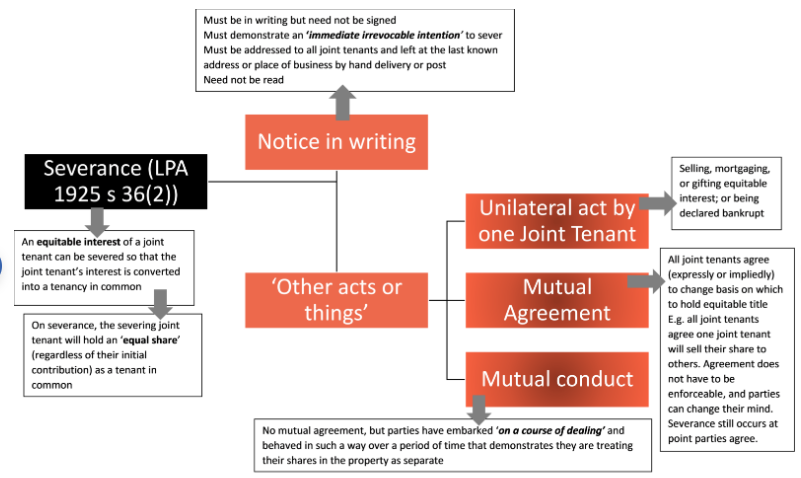
\includegraphics{C:/Users/shiva/Filen/MEGA/LegalPracticeCourse/severance-diagram.png}

The imposition of a trust involves the separation of legal and equitable
title. Legal title cannot be severed, but equitable title can be.

\hypertarget{definition-1}{%
\paragraph{Definition}\label{definition-1}}

\begin{quote}
Severance\ldots is the process of separating off the share of a joint
tenant, so that the concurrent ownership will continue, but the right of
survivorship will no longer apply. The parties will hold separate shares
as tenants in common.\\
Dillon LJ in Harris v Goddard {[}1983{]} 1 WLR 1203
\end{quote}

\begin{env-881a4bd6-779e-4404-ae5b-86f77846f864}

Note

Severance does not destroy co-ownership but simply changes the basis on
which the parties hold the equitable interest in the future.

\end{env-881a4bd6-779e-4404-ae5b-86f77846f864}

\hypertarget{details}{%
\paragraph{Details}\label{details}}

\begin{itemize}
\tightlist
\item
  Legal title

  \begin{itemize}
  \tightlist
  \item
    Maximum of 4 Trustees (i.e., 4 legal owners registered at the Land
    Registry)
  \item
    All must be `sui juris' (+18 and of sound mind)
  \item
    Must hold as joint tenants. This means the 4 unities must be present
    and the right of survivorship applies.
  \item
    The joint tenancy cannot be severed
  \end{itemize}
\item
  Equitable title

  \begin{itemize}
  \tightlist
  \item
    Unlimited number can hold
  \item
    Can be held by U18's and those that lack mental capacity
  \item
    Can be held as joint tenancy or tenancy in common
  \item
    Equitable joint tenancy can be severed into tenancy in common.
  \end{itemize}
\end{itemize}

If a beneficial (equitable) joint tenancy is created, it is open to any
joint tenant to sever that joint tenancy to create a tenancy in common.
A joint tenant may want to so this in order to exclude the operation of
survivorship, so that a distinct share in the property can be left to
someone other than the surviving joint tenant(s) on death. This may be
required because there has been a breakdown in the relationship between
the joint tenants, meaning that one person does not wish the other to
take the property by survivorship. However, sometimes the joint tenancy
is severed because, for example, the parties wish to enter a
tax-planning scheme which requires survivorship to be ruled out.

It is important to understand that severance does not bring co-ownership
to an end: it simply changes the basis on which the equitable co-owners
continue to hold the equitable title. Severance is the process of
converting an equitable interest held as a joint tenancy into an
interest held as a tenancy in common.

\begin{env-9843ce55-0506-497d-95ba-03a690b05b3c}

s 36(2) LPA 1925

No severance of a joint tenancy of a legal estate, so as to create a
tenancy in common in land, shall be permissible, whether by operation of
law or otherwise, but this subsection does not affect the right of a
joint tenant to release his interest to the other joint tenants, or the
right to sever a joint tenancy in an equitable interest whether or not
the legal estate is vested in the joint tenants:

Provided that, where a legal estate (not being settled land) is vested
in joint tenants beneficially, and any tenant desires to sever the joint
tenancy in equity, he shall give to the other joint tenants a notice in
writing of such desire or do such other acts or things as would, in the
case of personal estate, have been effectual to sever the tenancy in
equity, and thereupon the land shall be held in trust on terms which
would have been requisite for giving effect to the beneficial interests
if there had been an actual severance.

Nothing in this Act affects the right of a survivor of joint tenants,
who is solely and beneficially interested, to deal with his legal estate
as if it were not held in trust.

\end{env-9843ce55-0506-497d-95ba-03a690b05b3c}

It is not possible to sever a legal joint tenancy; only an equitable
one. This is to preserve the simplicity of the legal title. If legal
trustees could sever the joint tenancy and leave an interest held as a
tenancy in common to other(s), that would complicate the legal title for
two reasons: first, the number of legal owners could grow, not shrink!
Second, documents would be required to prove that the new holders had
actually acquired title properly. With a joint tenancy, the only
document required on the death of a joint tenant is a copy of that
person's death certificate.

\hypertarget{methods-of-severing}{%
\paragraph{Methods of Severing}\label{methods-of-severing}}

S 36(2) also states that the equitable joint tenancy can be severed and
states two basic ways that this can happen:

\begin{enumerate}
\tightlist
\item
  The severing joint tenant can give a \textbf{notice in writing} to all
  of the other equitable joint tenants.

  \begin{itemize}
  \tightlist
  \item
    The writing can be in any form and need not be signed.
  \item
    It must, however, demonstrate an unequivocal and irrevocable
    intention to sever the equitable joint tenancy immediately.
  \item
    Notice must also be served correctly if it is to have effect:

    \begin{itemize}
    \tightlist
    \item
      It must be given to all of the other equitable joint tenants
    \item
      The notice can be handed over or left at the last known place of
      abode or business of the other joint tenants
    \end{itemize}
  \item
    Case law makes it clear that the notice does not have to be read to
    be effective and severance takes place the moment the notice is
    served
  \end{itemize}
\item
  The joint tenant can do \textbf{`other acts or things'}, or behave in
  such a way that the joint tenancy is severed.

  \begin{itemize}
  \tightlist
  \item
    This piece of statute, deliberately vague, was intended so that the
    modes of severance recognised by Williams v Hensman (1861) 1 J \& H
    546 would continue to apply.
  \item
    In Williams v Hensmen, three possible ways in which a joint tenancy
    in personal property and land could be severed were identified.
    These 3 ways falls under the `other acts of things' mode of
    severance in s 36(2).
  \end{itemize}

  \begin{enumerate}
  \tightlist
  \item
    The first of these is a unilateral act by a joint tenant operating
    on his own share.

    \begin{itemize}
    \tightlist
    \item
      The most important point to note here is that the act can be
      unilateral: there is no requirement for the other joint tenant(s)
      to know or consent to the act for severance to take place.
    \item
      The unilateral act can be subdivided into 3 types of alienation.

      \begin{enumerate}
      \tightlist
      \item
        Total alienation

        \begin{itemize}
        \tightlist
        \item
          Acts of `total' alienation occur when the severing owner
          disposes of the interest permanently, by way of sale or gift
          of the equitable interest in land.
        \item
          For example, It is very common for one joint tenant to `buy
          out' another. The sale will have the effect of severing the
          equitable joint tenancy, and the purchaser will acquire the
          interest as a tenant in common.
        \end{itemize}
      \item
        Partial alienation

        \begin{itemize}
        \tightlist
        \item
          Acts of `partial' alienation occur where the severing owner
          temporarily disposes of the interest, by way of mortgage or
          lease. This is partial alienation because when the loan is
          repaid or the lease expires, the holder will take the interest
          back unencumbered.
        \item
          If an equitable joint tenant mortgages his or her equitable
          interest, that will be an act of severance, resulting in a
          tenancy in common. Please do not get confused with a legal
          mortgage, which would be where the joint tenants together
          charge the legal estate.
        \end{itemize}
      \item
        Involuntary alienation

        \begin{itemize}
        \tightlist
        \item
          occurs when a joint tenant is declared bankrupt by the court.
          It is `involuntary' as this will happen against the will of
          the joint tenant.
        \item
          If one of the co-owners is declared bankrupt, this will also
          operate to automatically sever their equitable interest in the
          land, which vests in the trustee in bankruptcy.
        \end{itemize}
      \end{enumerate}
    \end{itemize}
  \item
    Mutual agreement of joint tenants

    \begin{itemize}
    \tightlist
    \item
      Severance by mutual agreement will occur only when all equitable
      joint tenants agree that one person's interest is severed, thereby
      creating a tenancy In common.
    \item
      The agreement need not go as far as being a specifically
      enforceable contract to sell the interest; but it must amount to
      an agreement that one person's interest is separate or severed.
    \end{itemize}
  \item
    Mutual conduct (any course of dealing which indicates that interests
    were mutually treated as constituting a tenancy in common)

    \begin{itemize}
    \tightlist
    \item
      There is real overlap here with mutual agreement, and it is not
      always clear where the dividing line lies.
    \item
      If you cannot point to any moment where the parties have reached a
      mutual agreement, there may still be severance by mutual conduct.
    \item
      For example, if the parties have been negotiating over a prolonged
      period of time, then their conduct may suggest that they do
      recognise and are treating one person's interest as being
      separate. It will always be dependent on the facts of the case in
      hand, and the reality is that this mode of severance is hard to
      prove.
    \end{itemize}
  \end{enumerate}
\end{enumerate}

The severance must take place during the joint tenant's lifetime. Making
a will does not sever a joint tenancy as it takes effect after death,
whereas severance takes place immediately on death: Re Caines deceased
{[}1978{]} 1 WLR 540.

\hypertarget{effect-of-severance}{%
\paragraph{Effect of Severance}\label{effect-of-severance}}

If a joint tenant successfully severs the equitable joint tenancy, that
person will, in future, hold a tenancy in common which is an equal
share, based on the number of former joint tenants not on the proportion
of contributions made to the initial price: Goodman v Gallant {[}1986{]}
Fam 106.

\begin{env-de3101d4-f08b-48eb-bc0e-2fa06f3bcf8e}

Example

A, B, C and D are the legal owners of property, which they hold on trust
for themselves and E and F as joint tenants in equity. D wishes to sever
the joint tenancy so that he can leave his share of the property to G in
his will.

It is not possible to sever the legal joint tenancy, so D will continue
to have the administrative responsibilities of a legal trustee. The
equitable joint tenancy can be severed, and if D does this by one of the
methods recognised in \textbf{LPA s 36(2)}, D will have a one-sixth
separate equitable share as tenant in common.

\begin{itemize}
\tightlist
\item
  A B C and D hold legal title as joint tenants.
\item
  A B C E F hold 5/6 as JTs.
\item
  D has 1/6 as TIC.
\end{itemize}

\end{env-de3101d4-f08b-48eb-bc0e-2fa06f3bcf8e}

\begin{env-de3101d4-f08b-48eb-bc0e-2fa06f3bcf8e}

Example

A and B are the legal owners of property, which they hold on trust for
themselves as joint tenants in equity. B wishes to sever the joint
tenancy so that he can leave his share of the property to C in his will.

It is not possible to sever the legal joint tenancy, so B will continue
to have the administrative responsibilities of a legal trustee. The
equitable joint tenancy can be severed, and if B does this by one of the
methods recognised in LPA s 36(2), A and B will each have a 50\%
equitable share as tenant in common. It is not possible for A to
continue as a joint tenant.

\begin{itemize}
\tightlist
\item
  A and B hold legal title as joint tenants.
\item
  A and B hold 50\% each as TIC.
\end{itemize}

\end{env-de3101d4-f08b-48eb-bc0e-2fa06f3bcf8e}

MERMAID3

\hypertarget{notice-in-writing}{%
\paragraph{Notice in Writing}\label{notice-in-writing}}

S 36(2) states that the equitable joint tenancy can be severed. One way
this can be done is for the severing joint tenant to give a notice in
writing to all of the other equitable joint tenants.

Rules concerning the content and service of such notices must be
observed if the notice is to have the effect of severing the joint
tenancy.

The writing could be deliberately intended to sever the joint tenancy,
such as where it is the starting point to a tax planning scheme.
However, writing which is primarily intended for another purpose could
have the unintended consequence of severing the joint tenancy.

\hypertarget{form-and-intention}{%
\subparagraph{Form and Intention}\label{form-and-intention}}

There are no particular formalities to be observed for the notice: it
does not even need to be signed. However, it must demonstrate an
unequivocal and irrevocable intention to sever the equitable joint
tenancy immediately.

Two cases with similar facts, but different results demonstrate the
`intention' aspect perfectly. In each, one co-owner had died, and the
dispute had arisen between the surviving co-owner and the deceased's
next of kin. The surviving co-owner argued that the deceased had died as
a joint tenant and that they took the property by survivorship. The next
of kin argued that the deceased died as a tenant in common and that the
share passed to them.

\begin{itemize}
\tightlist
\item
  Re Draper's Conveyance {[}1969{]} 1 Ch 486
\item
  Harris v Goddard {[}1983{]} 1 WLR 1203
\item
  Quigley v Masterson {[}2011{]} EWHC 2529
\end{itemize}

\hypertarget{service}{%
\subparagraph{Service}\label{service}}

A notice in writing must be served correctly in order to sever the joint
tenancy. Section 36(2) makes it clear that the severing joint tenant
must `give to the other joint tenants' a notice in writing. It must
therefore be served on all of the other equitable joint tenants. In the
vast majority of cases this does not present a problem as there are only
two joint tenants to start with, but if there are more, then all must be
served.

Difficulties regarding when and whether a notice has been properly
served are resolved by \textbf{Law of Property Act 1925, s 196(3) and s
196(4)} and related case law.

\begin{env-9843ce55-0506-497d-95ba-03a690b05b3c}

s 196 LPA 1925

(1) Any notice required or authorised to be served or given by this Act
shall be in writing.

(2) Any notice required or authorised by this Act to be served on a
lessee or mortgagor shall be sufficient, although only addressed to the
lessee or mortgagor by that designation, without his name, or generally
to the persons interested, without any name, and notwithstanding that
any person to be affected by the notice is absent, under disability,
unborn, or unascertained.

(3) Any notice required or authorised by this Act to be served shall be
sufficiently served if it is left at the last-known place of abode or
business in the United Kingdom of the lessee, lessor, mortgagee,
mortgagor, or other person to be served, or, in case of a notice
required or authorised to be served on a lessee or mortgagor, is affixed
or left for him on the land or any house or building comprised in the
lease or mortgage, or, in case of a mining lease, is left for the lessee
at the office or counting-house of the mine.

(4) Any notice required or authorised by this Act to be served shall
also be sufficiently served, if it is sent by post in a registered
letter addressed to the lessee, lessor, mortgagee, mortgagor, or other
person to be served, by name, at the aforesaid place of abode or
business, office, or counting-house, and if that letter is not returned
{[}F1by the postal operator (within the meaning of {[}F2Part 3 of the
Postal Services Act 2011{]}) concerned{]} undelivered; and that service
shall be deemed to be made at the time at which the registered letter
would in the ordinary course be delivered.

\end{env-9843ce55-0506-497d-95ba-03a690b05b3c}

A notice can be served by handing it over personally. If it is posted it
will be deemed to be served if it has been left at the `last known place
of abode or business' of the joint tenants. This means that it could be
served by the severing joint tenant leaving it there, or by postal
delivery there. If it is made by registered post and not returned
undelivered, it will be deemed served at the time a registered item
would in the ordinary course of events be delivered.

Note that the provision says that the notice is deemed to have been
served when it has been delivered. It does not say that the notice has
to be received or read.

\begin{itemize}
\tightlist
\item
  Kinch v Bullard {[}1999{]} 1 WLR 423
\item
  Re 88 Berkeley Road {[}1971{]} Ch 648
\end{itemize}

\hypertarget{other-acts-or-things}{%
\paragraph{Other Acts or Things}\label{other-acts-or-things}}

S 36(2) states that the equitable joint tenancy can be severed. One way
this can be done is by other acts or things which would have the effect
of severing a joint tenancy in personal property.

In Williams v Hensman (1861) 1 J \& H 546 Page-Wood VC identified three
possible ways in which a joint tenancy in personal property and land
could be severed:

(1) A unilateral act by a joint tenant operating on his own share\\
(2) Mutual agreement of the joint tenants\\
(3) Any course of dealing which indicates that the interests were
mutually treated as constituting a tenancy in common.

\hypertarget{unilateral-act-by-one-joint-tenant}{%
\subparagraph{Unilateral Act by One Joint
Tenant}\label{unilateral-act-by-one-joint-tenant}}

There is a logical inconsistency in saying that a joint tenancy can be
severed by one joint tenant `acting on his own share' as we already know
that the joint tenant does not have a `share' in the first place.
However we can interpret this as meaning that the act itself creates the
share: it does not exist unless and until the act takes place.

The most important point to note here is that the act can be unilateral:
there is no requirement for the other joint tenant(s) to know or consent
to the act for severance to take place.

The unilateral acts can be subdivided into acts of total alienation;
partial alienation; and involuntary alienation.

\begin{itemize}
\tightlist
\item
  Total alienation: acts of `total' alienation occur when the severing
  owner disposes of the interest permanently, by way of sale or gift of
  the interest.
\item
  Partial alienation: acts of `partial' alienation occur where the
  severing owner temporarily disposes of the interest, by way of
  mortgage or lease. This is partial alienation because when the loan is
  repaid or the lease expires, the holder will take the interest back
  unencumbered.
\item
  Involuntary alienation: this occurs when the joint tenant is declared
  bankrupt by the court. It is `involuntary' as this will happen against
  the will of the joint tenant!
\end{itemize}

\begin{env-de3101d4-f08b-48eb-bc0e-2fa06f3bcf8e}

Sale as an act of total alienation

It is very common for one joint tenant to `buy out' another. The sale
will have the effect of severing the equitable joint tenancy and the
purchaser will acquire the interest as a tenant in common. The legal
title will remain unaffected as the legal joint tenancy cannot be
severed. Imagine that A B C and D own property as beneficial joint
tenants. B has been offered a job in another city and sells his
equitable interest to C.

Position before the sale: the usual rules on co-ownership operate and
ABC \& D are legal joint tenants holding the property on trust for
themselves as equitable joint tenants.

Position after the sale: ABC \& D continue as legal joint tenants as the
legal title cannot be severed. B's equitable interest is severed on sale
to C, who holds it as a tenant in common. C remains a joint tenant with
A \& D as to the remaining equitable title.

\end{env-de3101d4-f08b-48eb-bc0e-2fa06f3bcf8e}

\begin{env-de3101d4-f08b-48eb-bc0e-2fa06f3bcf8e}

Mortgage as an act of partial alienation

Most property purchases are funded by mortgage finance. Where all legal
joint tenants act together to create a legal mortgage or charge over the
property as security for a loan, this does not result in severance,
because the joint tenants are charging the legal estate. The equitable
estate remains unaffected.

If an equitable joint tenant mortgages his/her equitable interest, that
will be an act of severance, resulting in a tenancy in common.

Where one joint tenant fraudulently tries to mortgage/sell the entire
property. In this case, the disposition is deemed to be a mortgage/sale
of the equitable interest.

\end{env-de3101d4-f08b-48eb-bc0e-2fa06f3bcf8e}

See First National Security v Hegarty {[}1985{]} QB 850

\hypertarget{mutual-agreement}{%
\subparagraph{Mutual Agreement}\label{mutual-agreement}}

Severance by mutual agreement will occur only when all equitable joint
tenants agree that one person's interest is severed, thereby creating a
tenancy in common. The agreement need not go as far as the `unilateral
acts' operating on a share. The agreement need not go as far as being a
specifically enforceable contract to sell the interest; but it must
amount to an agreement that one person's interest is separate or
severed.

This mode of severance is closely linked to severance by mutual conduct,
and it is unclear where the dividing line lies. The leading case here is
Burgess v Rawnsley {[}1975{]} Ch 429.

Hunter v Babbage (1995) 69 P\&CR 548

\hypertarget{mutual-conduct}{%
\subparagraph{Mutual Conduct}\label{mutual-conduct}}

Where the parties have not reached a point where there can be said to be
`mutual agreement' to sever the joint tenancy, there may still be
severance by `mutual conduct'. In Williams v Hensman (1861) 1 J \& H 546
Page-Wood VC defined mutual conduct as:

\begin{quote}
` any course of dealing sufficient to intimate that the interests of all
were mutually treated as constituting a tenancy in common\ldots'
\end{quote}

The question of severance by mutual conduct is most likely to arise
where the parties have not reached a point where there could be said to
be a `mutual agreement' to sever. However the fact that they are
negotiating over a prolonged period of time suggests that they do
recognise and are treating one person's interest as being separate.

In Burgess v Rawnsley {[}1975{]} Ch 429, Sir John Pennycuick
acknowledged that severance could be inferred from negotiations, but
this was obiter as the decision in that case was made on the basis of
mutual agreement. The reality is that it will prove difficult to show
that there has been severance by mutual conduct, as the fact that the
negotiations are ongoing means that it is unlikely that there is any
mutuality at all!

See Gore and Snell v Carpenter {[}1990{]} 60 P\&CR 456 and Davis v Smith
{[}2011{]} EWCA Civ 1603.

\begin{env-d6ce83a0-f7a8-46b6-be95-b1235f1feb63}

Summary

\textbf{Law of Property Act 1925, s 36(2)} states that an equitable
joint tenancy can be severed by `other acts or things\ldots'.

According to the case of \textbf{Williams v Hensman} this behaviour can
be unilateral acts, mutual agreement or mutual conduct.

Examples of unilateral acts operating on a share include selling,
mortgaging, or gifting a share; or being declared bankrupt.

Severance by mutual agreement occurs when the joint tenants all agree,
expressly or impliedly, to change the basis on which they continue to
hold the equitable title to the property

Severance by mutual conduct may occur when the parties embark on a
`course of dealings' which demonstrates that they are treating their
shares in the property as separate. This may cover ongoing negotiations,
but it is unclear exactly what will suffice here.

\end{env-d6ce83a0-f7a8-46b6-be95-b1235f1feb63}

\hypertarget{bevan-1}{%
\paragraph{Bevan}\label{bevan-1}}

Concurrent ownership is one of the most common forms of land holding,
and poses many challenges. The law must finely balance all parties'
interests, and the interests of co-owners against any creditors. Two
fundamental features:

\begin{itemize}
\tightlist
\item
  The distinguishing feature of co-ownership is ``unity of possession'',
  meaning each co-owner enjoys an entitlement to possess the co-owned
  land.
\item
  Under English law, all forms of shared ownership must operate behind a
  trust, so wherever there is co-ownership, a trust will arise. This
  involves the separation of the formal legal title to land from the
  underlying equitable ownership of the land.
\end{itemize}

The two forms of co-ownership recognised in English law today are the
joint tenancy and tenancy in common.

\hypertarget{joint-tenancy-1}{%
\subparagraph{Joint Tenancy}\label{joint-tenancy-1}}

Each co-owner is regarded as wholly entitled to the land. No single
co-owner has any 'share' in the co-owned land, and collectively all
co-owners are treated as a single unit. If there is an express
declaration of joint tenancy, this will give rise to a joint tenancy
even if the contributions to the purchase price are unequal.

A joint tenancy can only exist where the four unities are present. These
are:

\begin{itemize}
\tightlist
\item
  Unity of possession
\item
  Unity of interest
\item
  Unity of title
\item
  Unity of time
\end{itemize}

The most important practical significance of co-ownership under a joint
tenancy is that between joint tenants, the doctrine of survivorship
(\emph{ius accrescendi}) operates. When one joint tenant dies, her
interest automatically passes to or 'survives to' the remaining joint
tenants. This operates automatically upon death, and takes precedence
over the terms of a will.

When all but one joint tenant has deceased, the remaining joint tenant
is no longer a co-owner and becomes absolutely entitled to the land.
What if the final surviving joint tenants die simultaneously? Then the
younger will be deemed to have survived the older (s 184 LPA 1925).

Survivorship has several advantages:

\begin{enumerate}
\tightlist
\item
  Often reflects the wishes of parties
\item
  Simplifies probate
\item
  Simplifies purchases of co-owned land (only one title vested in
  several joint tenants).
\end{enumerate}

\hypertarget{tenancy-in-common-1}{%
\subparagraph{Tenancy in Common}\label{tenancy-in-common-1}}

Joint tenants can separate their interest from other joint tenants
through the process of severance. This transforms a joint tenant's
interest in the co-owned land into a notional share of the co-owned
land, and that co-owner becomes a tenant in common. The size of the
share is calculated as a proportion of the total number of co-owners. On
death, the interest of the tenant in common does not survive
automatically to the remaining co-owners; the co-owner is free to
bequeath her interest to her heirs. A tenant in common is even able to
sell or mortgage their share. Only unity of possession is needed for a
tenancy in common to arise.

\hypertarget{position-in-law}{%
\subparagraph{Position in Law}\label{position-in-law}}

\begin{itemize}
\tightlist
\item
  At law, co-ownership can only exist under a joint tenancy. There can
  be no tenancy in common at law
  (\href{https://www.legislation.gov.uk/ukpga/Geo5/15-16/20/section/1}{s
  1(6) LPA 1925}).
\item
  Consequently, there can be no severance of a joint tenancy at law
  (\href{https://www.legislation.gov.uk/ukpga/Geo5/15-16/20/section/36}{s
  36(2) LPA 1925}). This does not affect a joint tenant's ability to
  'release' her interest to the other joint tenants and simply drop out
  of legal co-ownership of land.
\item
  There can be no more than four legal co-owners of land
  (\href{https://www.legislation.gov.uk/ukpga/Geo5/15-16/20/section/34}{s
  34(2) LPA 1925}) -- though in equity, there is no limit on the number
  of co-owners that can exist nor any rule against co-owners under 18.
\end{itemize}

\hypertarget{position-in-equity}{%
\subparagraph{Position in Equity}\label{position-in-equity}}

Co-ownership in equity is far more flexible: co-owners may be either
joint tenants or tenants in common. To determine which category
co-owners fall into, consider:

\begin{enumerate}
\tightlist
\item
  Any express declarations of trust
\item
  The presence of the four unities
\item
  The application of various equitable presumptions.
\end{enumerate}

Express Declaration of Trust

An express declaration may indicate how the property is to be held in
equity. A clear expression of intention will be conclusive and not
usurped by any implication drawn on the facts (though it could be
usurped by vitiating factors, e.g., fraud) -- Goodman v Gallant
{[}1986{]} Fam 106, Pankhania v Chandegra {[}2012{]} EWCA Civ 1438

\hypertarget{rights-and-duties-of-trustees-and-beneficiaries}{%
\subsubsection{Rights and Duties of Trustees and
Beneficiaries}\label{rights-and-duties-of-trustees-and-beneficiaries}}

All co-owned land is held under a trust of land.

The trust is governed by the
\href{https://www.legislation.gov.uk/ukpga/1996/47/contents}{Trusts of
Land and Appointment of Trustees Act 1996} (TLATA 1996). The Act governs
the way the trust of land operates and confers rights and powers on both
trustees and beneficiaries, and sets out the duties of the trustees.

When looking at the provisions of \textbf{TLATA 1996} it must be
remembered that the statute does not simply cover trusts which arise as
a result of land being co-owned. Many of the provisions apply to trusts
of land set up in wills, or express lifetime trusts created by a
settlor.

\hypertarget{powers-and-duties-of-trustees}{%
\paragraph{Powers and Duties of
Trustees}\label{powers-and-duties-of-trustees}}

The legal title to land is vested in the trustees who have the powers of
an absolute owner:
\href{https://www.legislation.gov.uk/ukpga/1996/47/section/6}{TLATA
1996, s 6(1)}. This means that they can sell, mortgage, lease, grant
easements and so on. However, the power is not absolute: the trustees
have the powers of an absolute owner subject to the brakes imposed in
the Act.
\href{https://www.legislation.gov.uk/ukpga/1996/47/section/6}{TLATA
1996, s 6(5)} says that the trustees must have regard to the rights of
the beneficiaries when exercising their powers, and act in accordance
with the duty of care imposed in
\href{https://www.legislation.gov.uk/ukpga/1996/47/section/6}{TLATA
1996, s 6(9)} and
\href{https://www.legislation.gov.uk/ukpga/2000/29/section/1}{Trustee
Act 2000 s 1}.

One of the most important brakes on the trustee's powers is contained in
\href{https://www.legislation.gov.uk/ukpga/1996/47/section/11}{TLATA
1996, s 11}. The trustees must, in the exercise of any function relating
to the land, so far as practicable consult the beneficiaries of full
age, and so far as is consistent with the general interest of the trust,
give effect to the wishes of those beneficiaries or, in the case of a
dispute, to the wishes of the majority by value of the combined
interests.

This means that if the trustees wish to sell the property they are
obliged to consult the beneficiaries, but need not give effect to their
wishes unless it is deemed to be in the general interest of the trust.

\begin{env-9843ce55-0506-497d-95ba-03a690b05b3c}

s 6 TLATA 1996

(1) For the purpose of exercising their functions as trustees, the
trustees of land have in relation to the land subject to the trust all
the powers of an absolute owner.

(2) Where in the case of any land subject to a trust of land each of the
beneficiaries interested in the land is a person of full age and
capacity who is absolutely entitled to the land, the powers conferred on
the trustees by subsection (1) include the power to convey the land to
the beneficiaries even though they have not required the trustees to do
so; and where land is conveyed by virtue of this subsection---

\begin{itemize}
\item
  (a) the beneficiaries shall do whatever is necessary to secure that it
  vests in them, and
\item
  (b) if they fail to do so, the court may make an order requiring them
  to do so.
\end{itemize}

(3) The trustees of land have power to acquire land under the power
conferred by section 8 of the Trustee Act 2000.

(5) In exercising the powers conferred by this section trustees shall
have regard to the rights of the beneficiaries.

(6) The powers conferred by this section shall not be exercised in
contravention of, or of any order made in pursuance of, any other
enactment or any rule of law or equity.

(7) The reference in subsection (6) to an order includes an order of any
court or of the Charity Commission.

(8) Where any enactment other than this section confers on trustees
authority to act subject to any restriction, limitation or condition,
trustees of land may not exercise the powers conferred by this section
to do any act which they are prevented from doing under the other
enactment by reason of the restriction, limitation or condition.

(9) The duty of care under section 1 of the Trustee Act 2000 applies to
trustees of land when exercising the powers conferred by this section.

\end{env-9843ce55-0506-497d-95ba-03a690b05b3c}

\begin{env-d6ce83a0-f7a8-46b6-be95-b1235f1feb63}

Summary

Trustees - hold legal title

\begin{itemize}
\tightlist
\item
  Have the powers of an absolute owner (s 6(1)) but must have regard to
  the rights of the beneficiaries (s 6(5))
\item
  Duty of care imposed in s 6(9) and Trustee Act 2000 s 1
\item
  Duty to consult beneficiaries of full age and give effect to the
  wishes of those beneficiaries or, in the case of a dispute, to the
  wishes of the majority by value of the combined interests.
\end{itemize}

\end{env-d6ce83a0-f7a8-46b6-be95-b1235f1feb63}

\hypertarget{rights-of-beneficiaries}{%
\paragraph{Rights of Beneficiaries}\label{rights-of-beneficiaries}}

Before TLATA 1996 was enacted, beneficiaries' interests were regarded as
being in the proceeds of sale of land and not in land itself. This is
known as the doctrine of conversion, whereby the interests were seen as
being personal interests in money even though there had been no sale!

\href{https://www.legislation.gov.uk/ukpga/1996/47/section/3}{TLATA
1996, s 3} abolished the doctrine of conversion and beneficiaries now
enjoy proprietary interests in the land itself. They have two main
rights: the right to be consulted and the right to occupy trust land,
but these rights are hedged and bound by qualifications.

As has been seen, the trustees hold the land for the beneficiaries and
the trustees' powers are to be exercised in their best interests. The
trustees owe the beneficiaries a duty of care:
\href{https://www.legislation.gov.uk/ukpga/1996/47/section/1}{TLATA
1996, s 1}, and
\href{https://www.legislation.gov.uk/ukpga/1996/47/section/6}{s 6(5)}
obliges the trustees to have regard to the rights of the beneficiaries
when exercising their powers. They must also, in the exercise of any
function, consult the beneficiaries, but need not give effect to their
wishes unless it is deemed to be in the general interest of the trust:
\href{https://www.legislation.gov.uk/ukpga/1996/47/section/11}{TLATA
1996, s 11}.

The right to be consulted is very important if the beneficiaries' views
are to be heard, especially in trusts of land where equitable owners are
not also legal owners. However, as stated above, the trustees are not
obliged to act on their wishes.

\hypertarget{right-to-occupy}{%
\subparagraph{Right to Occupy}\label{right-to-occupy}}

Beneficiaries have a right to occupy trust property:
\href{https://www.legislation.gov.uk/ukpga/1996/47/section/12}{TLATA
1996, s 12}. The right will only arise where two criteria are met:

\begin{enumerate}
\tightlist
\item
  It must be shown that the land was intended for occupation by those
  beneficiaries: TLATA 1996, s 12(1).
\item
  It must be shown that the land is suitable for occupation by the
  particular beneficiaries: TLATA 1996, s 12(2).
\end{enumerate}

\begin{env-9843ce55-0506-497d-95ba-03a690b05b3c}

s 12 TLATA 1996

(1) A beneficiary who is beneficially entitled to an interest in
possession in land subject to a trust of land is entitled by reason of
his interest to occupy the land at any time if at that time---

\begin{itemize}
\item
  (a) the purposes of the trust include making the land available for
  his occupation (or for the occupation of beneficiaries of a class of
  which he is a member or of beneficiaries in general), or
\item
  (b) the land is held by the trustees so as to be so available.
\end{itemize}

(2) Subsection (1) does not confer on a beneficiary a right to occupy
land if it is either unavailable or unsuitable for occupation by him.

(3) This section is subject to section 13.

\end{env-9843ce55-0506-497d-95ba-03a690b05b3c}

It is clear from above that where a couple owns a home jointly, each
will have the right to occupy it, as the property is both intended and
suitable for occupation by them.

However, if the land was bought as an investment, say as a buy-to-let
property, then there may be no right to occupy, as it was not intended
for occupation by beneficiaries.

Note that TLATA 1996, s 12(2) states that there is no right to occupy if
the land is unsuitable for occupation by a beneficiary. The land does
not have to be unsuitable for occupation altogether, it must simply be
unsuitable for occupation by that particular beneficiary. For example,
land which is a farm may not be suitable for occupation by a beneficiary
who is not a farmer.

\hypertarget{restrictions}{%
\subparagraph{Restrictions}\label{restrictions}}

If two or more beneficiaries have a right to occupy the same land, the
trustees can exclude or restrict the right for one or more, but not all,
of them:
\href{https://www.legislation.gov.uk/ukpga/1996/47/section/13}{TLATA
1996, s 13(1)}; although they may not unreasonably exclude any
beneficiary, or restrict to an unreasonable extent:
\href{https://www.legislation.gov.uk/ukpga/1996/47/section/13}{TLATA
1996, s 13(2)}.

In exercising the power to exclude or restrict, the trustees must have
regard to the purpose for which the land was bought, and the
circumstances and wishes of each beneficiary who is entitled to occupy:
\href{https://www.legislation.gov.uk/ukpga/1996/47/section/13}{TLATA
1996, s 13(4)}.

The trustees may impose conditions such as paying outgoings and
expenses, on beneficiaries in occupation: TLATA 1996, s 13(3) ands
13(6). If a beneficiary has been excluded, the trustees may require the
occupying beneficiaries to pay compensation to him/them: TLATA 1996, s
13(6).

If a beneficiary is already in occupation of the land, the trustees
cannot exercise their powers so as to exclude that person, nor in a
manner likely to make the beneficiary leave, unless the beneficiary
consents or the court approves.

These provisions weaken the apparently strong right to occupy
considerably.

\begin{env-d6ce83a0-f7a8-46b6-be95-b1235f1feb63}

Summary

Beneficiaries - hold Equitable title

\begin{itemize}
\tightlist
\item
  Right to be consulted if 18+ (s 11)
\item
  Right to occupy the land (s 12) if the land was intended for and is
  suitable for occupation, but can be restricted if two or more
  beneficiaries have the right to occupy (s 13). Conditions can also be
  imposed, such as paying outgoings.
\end{itemize}

\end{env-d6ce83a0-f7a8-46b6-be95-b1235f1feb63}

\hypertarget{dispute-resolution}{%
\subsubsection{Dispute Resolution}\label{dispute-resolution}}

By its very nature, co-ownership involves two or more people owning the
same land at the same time. It is inevitable that there will be
differences of opinion affecting ownership, particularly as to whether
the land should be sold or not.

Where the trustees and the beneficiaries are different people, and the
land is owned as a commercial venture or as an investment, any
difference of opinion may be dealt with by the trustees using their
discretion.

However, where the property has been purchased as a home, and the
trustees and the beneficiaries being the same people whose relationship
has ended, the chances of any dispute being resolved amicably are much
reduced. Further, if one or more co-owners is in debt, the creditors may
wish to press for a sale of the property in order to recover the money
due to them, although the co-owners may not want this.

\hypertarget{tlata-1996}{%
\paragraph{TLATA 1996}\label{tlata-1996}}

Trusts of Land and Appointment of Trustees Act 1996 (TLATA 1996) does
not simply govern the way the trust of land operates. It also contains
provisions as to how disputes relating to land held in trust are to be
resolved.

\href{https://www.legislation.gov.uk/ukpga/1996/47/section/14}{TLATA
1996, s 14} gives courts jurisdiction to hear applications regarding
disputes which involve co-owned land. Anyone with an interest in the
land can apply to the court for an order relating to it.

\begin{env-9843ce55-0506-497d-95ba-03a690b05b3c}

s 14 TLATA 1996

(1) Any person who is a trustee of land or has an interest in property
subject to a trust of land may make an application to the court for an
order under this section.

(2) On an application for an order under this section the court may make
any such order---

\begin{itemize}
\tightlist
\item
  (a) relating to the exercise by the trustees of any of their functions
  (including an order relieving them of any obligation to obtain the
  consent of, or to consult, any person in connection with the exercise
  of any of their functions), or
\item
  (b) declaring the nature or extent of a person's interest in property
  subject to the trust,\\
  as the court thinks fit.
\end{itemize}

(3) The court may not under this section make any order as to the
appointment or removal of trustees.

(4) The powers conferred on the court by this section are exercisable on
an application whether it is made before or after the commencement of
this Act.

\end{env-9843ce55-0506-497d-95ba-03a690b05b3c}

\begin{itemize}
\tightlist
\item
  Applicants could be trustees; beneficiaries; mortgagees of the legal
  or equitable title; trustees in bankruptcy; people who hold charging
  orders etc.
\item
  The court may order trustees to do something eg: sell; or allow a
  beneficiary into occupation. It cannot order one beneficiary to `buy
  out' the another
\item
  Orders which may be made include orders for sale (which may be
  postponed); orders as to who occupies; and orders as to the nature or
  extent of a beneficiary's interest.
\end{itemize}

\hypertarget{court-decision-making}{%
\paragraph{Court Decision-making}\label{court-decision-making}}

The court must apply all factors in
\href{https://www.legislation.gov.uk/ukpga/1996/47/section/15}{s 15
TLATA 1996} in reaching its decision in relation to s 14 applications.
It cannot pick and choose which factors to apply: all relevant factors
must be considered equally. Each must be considered carefully and a
decision made as to whether it leans towards granting an application
for, say, an order for sale, or against it.

\begin{env-9843ce55-0506-497d-95ba-03a690b05b3c}

s 15 TLATA 1996

(1) The matters to which the court is to have regard in determining an
application for an order under section 14 include---

\begin{itemize}
\tightlist
\item
  (a) the intentions of the person or persons (if any) who created the
  trust,
\item
  (b) the purposes for which the property subject to the trust is held,
\item
  (c) the welfare of any minor who occupies or might reasonably be
  expected to occupy any land subject to the trust as his home, and
\item
  (d) the interests of any secured creditor of any beneficiary.
\end{itemize}

(2) In the case of an application relating to the exercise in relation
to any land of the powers conferred on the trustees by section 13, the
matters to which the court is to have regard also include the
circumstances and wishes of each of the beneficiaries who is (or apart
from any previous exercise by the trustees of those powers would be)
entitled to occupy the land under section 12.

(3) In the case of any other application, other than one relating to the
exercise of the power mentioned in section 6(2), the matters to which
the court is to have regard also include the circumstances and wishes of
any beneficiaries of full age and entitled to an interest in possession
in property subject to the trust or (in case of dispute) of the majority
(according to the value of their combined interests).

(4) This section does not apply to an application if section 335A of the
M1Insolvency Act 1986 (which is inserted by Schedule 3 and relates to
applications by a trustee of a bankrupt) applies to it.

\end{env-9843ce55-0506-497d-95ba-03a690b05b3c}

When we are considering co-owned land, we need not be concerned with the
factor in \textbf{TLATA 1996, s 15(a)} as this relates to expressly
created lifetime trusts, or will trusts, and not to everyday
co-ownership. It is where someone sits down to bequeath their assets
through a trust to create wealth for their family. TLATA 1996, s 15(b)
requires the court to consider: "the purposes for which the property
subject to the trust is held".

If that purpose is still continuing, it will weigh against an order for
sale being made. The contrasting cases In re Ever's Trust {[}1980{]} 1
WLR 1327 and Jones v Challenger {[}1961{]} 1 QB 176 illustrate this.

\begin{env-881a4bd6-779e-4404-ae5b-86f77846f864}

Note

These cases were decided under a different statutory regime, before
TLATA 1996 came into force, but there is no reason to think that, were
they to be decided today, the outcome would be any different.

\end{env-881a4bd6-779e-4404-ae5b-86f77846f864}

\hypertarget{s-15c}{%
\subparagraph{S 15(c)}\label{s-15c}}

TLATA 1996, s 15(c) requires the court to consider `the welfare of any
minor who occupies or might reasonably be expected to occupy any land
subject to the trust as his home'. This factor is heavily dependent on
circumstances. Children aged six and seven may well have great weight
attached to their welfare, with the continuity of their living
arrangements being given priority over the interests of the applicant
who wants a sale. On the other hand, a young person who is seventeen and
still a child for these purposes, but may well be at work, and
relatively independent. In that case, less weight will be given to their
interests.

\hypertarget{s-15d}{%
\subparagraph{S 15(d)}\label{s-15d}}

TLATA 1996, s 15(d) requires the court to consider `the interests of any
secured creditor of any beneficiary'.

The approach of the court to the interests of the creditor has changed
over time. Pre-TLATA 1996, the presumption was always in favour of a
sale, and the interests of the creditors tended to take precedence even
where there were children in the property and the purpose for which the
property was bought continued. Post-TLATA 1996 the interests of the
secured creditors are just one factor to be considered. There is no
presumption for or against a sale at the start. The new approach is
illustrated by Mortgage Corporation v Shaire {[}2001{]} Ch 743.

Further cases:

\begin{longtable}[]{@{}ll@{}}
\toprule()
Case & Summary \\
\midrule()
\endhead
Bank of Ireland Home Mortgages v Bell {[}2001{]} 2 FLR 809 & The Court
of Appeal ordered a sale. The purpose of a family home, and the
interests of a minor were not material factors, as Mr and Mrs Bell had
divorced and their son was almost 18. The bank was owed £300,000 and no
payment had been made for almost eight years. The level of debt was
rising daily. Without a sale the bank had no real prospect of recovering
anything, which the court felt was very unfair to the bank in the
circumstances. \\
C Putnam and Sons v Taylor {[}2009{]} EWCH 317 (Ch) & The secured
creditor of a husband was granted an order for sale of a jointly owned
property when his debts became unmanageable. The purpose of a family
home still continuing, but the court ordered the sale as the wife held
enough equity in the property to enable her to buy a smaller property
outright. \\
Fred Perry v Genis {[}2015{]} 1 P\&CR DG5 & A sale was ordered even
though the children's education at a specialist school would be
disrupted. The court specifically stated that commercial interests
should take precedence over the residential security of the family.
However it postponed the order for a year to give the family time to
relocate. \\
\bottomrule()
\end{longtable}

\hypertarget{s-153}{%
\paragraph{S 15(3)}\label{s-153}}

Finally, do not forget the general sweeper in s 15(3). The court must
have regard to the wishes of the beneficiaries who are over 18. If there
is a dispute, the court shall have regard to the majority (in respect of
value of interest held.)

\begin{env-d6ce83a0-f7a8-46b6-be95-b1235f1feb63}

Summary

\textbf{TLATA 1996 s 14} allows anyone with an interest in land to apply
to the court for an order in relation to that land.

The usual form of order requested is an order for sale of the property,
which can be postponed for a period of time.

In making its decision, the court must have regard to the criteria in
\textbf{TLATA 1996, s 15.}

All criteria should be weighed even-handedly: the purpose for which the
land was bought; the interests of minors; the interests of secured
creditors; and the circumstances and wishes of beneficiaries of full
age.

In practice, greater weight tends to be given to the interests of
creditors, especially where the debt has spiralled out of control, or
there is sufficient equity in the property to purchase an alternative.

\end{env-d6ce83a0-f7a8-46b6-be95-b1235f1feb63}

When land is co-owned, owned under a trust of land.

Two types:

\begin{itemize}
\tightlist
\item
  Joint tenancy (legal and equitable interest)
\item
  Tenancy in common (equitable interest).
\end{itemize}

\hypertarget{conduct-issues}{%
\section{Conduct Issues}\label{conduct-issues}}

Summary of conduct issues most likely to be encountered in a
conveyancing transaction.

\hypertarget{acting-for-seller-and-buyer}{%
\subsection{Acting for Seller and
Buyer}\label{acting-for-seller-and-buyer}}

\begin{env-d6ce83a0-f7a8-46b6-be95-b1235f1feb63}

Question

Can a solicitor act for both the buyer and seller in a conveyancing
transaction?

\end{env-d6ce83a0-f7a8-46b6-be95-b1235f1feb63}

Occasionally, the parties to a conveyancing transaction ask if one
solicitor or one firm of solicitors can act for both parties. The
parties usually request this as a way of saving duplication of time and
expense.

\hypertarget{basic-rule-1}{%
\subsubsection{Basic Rule}\label{basic-rule-1}}

para 6.2 SRA Codes, a solicitor or firm cannot act if the solicitor or
firm has a conflict of interest or significant of such a conflict.

Recall Conflicts of Interest: a conflict of interest is `a situation
where your separate duties to act in the best interests of two or more
clients conflict'.

Whilst the SRA Codes do not prohibit acting for both buyer and seller,
it is worth noting that guidance issued by the SRA notes this can give
rise to a conflict of interest or a significant risk of one.

\hypertarget{relevant-factors}{%
\subsubsection{Relevant Factors}\label{relevant-factors}}

Factors to take into account when determining whether a conflict of
interest exists, or is likely to arise, include:

\begin{enumerate}
\tightlist
\item
  the complexity of the matter and length of the conveyancing chain
  involved.
\item
  the likelihood of negotiations having to take place. In higher value
  or complex transactions, there is a greater likelihood of substantial
  contract negotiations, increasing the risk of a conflict;
\item
  the bargaining power of the parties and any particular vulnerability
  of either party.
\end{enumerate}

\hypertarget{exceptions}{%
\subsubsection{Exceptions}\label{exceptions}}

If there is a conflict, or a significant risk of one, the solicitor or
firm can only act for both parties if one of the two exceptions
contained in para 6.2 applies.

\begin{itemize}
\tightlist
\item
  Under para 6.2(a), a solicitor can act for more than one party even if
  there is a conflict where the clients have a `substantially common
  interest' in relation to a matter or a particular aspect of it and the
  conditions set out in para 6.2(i)--(iii) are satisfied.

  \begin{itemize}
  \tightlist
  \item
    According to the SRA Glossary, a `substantially common interest' is
    a situation where there is a clear common purpose between the
    clients and a strong consensus on how it is to be achieved.
  \item
    Law Society guidance issued in June 2020 states that this exception
    `does not apply to a property purchase. Although both clients have a
    common interest in completing the sale, they also have different
    interests, since one is buying and one is selling.'
  \end{itemize}
\item
  The other exception to the general prohibition in para 6.2 is
  contained in para 6.2(b) and applies when the clients are competing
  for the same objective.

  \begin{itemize}
  \tightlist
  \item
    This cannot apply to a seller and buyer in a conveyancing
    transaction as they are not competing for the same asset and
    therefore do not satisfy the definition of `competing for the same
    objective'.
  \end{itemize}
\end{itemize}

\begin{env-d6ce83a0-f7a8-46b6-be95-b1235f1feb63}

Summary

So a solicitor or firm may only act for both parties in a conveyancing
transaction in the rare instances where they are satisfied that there is
no existing conflict of interest and no significant risk of a conflict
arising in future, or there is a conflict of interest but the parties
share a substantially common interest. This will be difficult to
establish where the land or interest in land is being transferred for
value.

Many solicitors and firms therefore take the view that it is best never
to act for both buyer and seller in a property transaction, even where
this could be justified under the SRA Codes.

\end{env-d6ce83a0-f7a8-46b6-be95-b1235f1feb63}

\hypertarget{steps-to-take-if-you-act}{%
\subsubsection{Steps to Take if You
Act}\label{steps-to-take-if-you-act}}

If you do decide to act:

\begin{itemize}
\tightlist
\item
  Inform the clients in writing that should a conflict arise you will
  cease to act.
\item
  Obtain client's consent to the firm acting
\item
  Record the factors considered in reaching a decision.
\item
  Ensure that each party is represented by a different fee earner.
\end{itemize}

If a decision is made to act under the `substantially common interest'
exception then the conditions in para 6.2(i)--(iii) must be complied
with.

\hypertarget{acting-for-joint-buyers}{%
\subsection{Acting for Joint Buyers}\label{acting-for-joint-buyers}}

It is usually acceptable to act for joint buyers. It may be necessary to
advise residential buyers separately about their rights in property,
particularly when they are not married/ in civil partnership.

\hypertarget{acting-for-borrower-and-lender}{%
\subsection{Acting for Borrower and
Lender}\label{acting-for-borrower-and-lender}}

As soon as the buyer's solicitor receives instructions to act for the
lender, they are effectively acting for both parties in one transaction
(i.e., for both lender and borrower). They have two clients and owe a
duty to both (see Mortgage Express v Bowerman \& Partners (A Firm)
{[}1996{]} 2 All ER 836). Acting for borrower and lender is possible
unless, under para 6.2 of the SRA Codes, the solicitor or firm has a
conflict of interest or a significant risk of a conflict.

\begin{env-d6ce83a0-f7a8-46b6-be95-b1235f1feb63}

When might there be a conflict between a buyer and lender?

\begin{enumerate}
\tightlist
\item
  The terms of the mortgage offer are unfair to the borrower (e.g., an
  extortionate rate of interest is being charged);
\item
  Instructions reveal that the buyer would be in breach of one of the
  terms of the offer (e.g., by allowing tenants into possession of the
  property);
\item
  The buyer is unable to comply with the lender's terms (e.g., to
  provide the balance of the purchase price from his own funds);
\item
  The mortgage documentation requires negotiation between the parties
  (but see below).
\end{enumerate}

\end{env-d6ce83a0-f7a8-46b6-be95-b1235f1feb63}

Note that (4) is more finely balanced. In residential transactions, the
borrower will often be borrowing from a high street bank or building
society, where the mortgage is offered on standard terms and conditions.
Arguably, there is either no conflict of interest or, if there is, there
is a `substantially common interest' under para 6.2 in that both the
borrower and the lender want a good and marketable title to the property
to be acquired.

\begin{env-785438bb-4d67-4370-80ef-9aa959fc6b60}

Law Society guidance (June 2020)

It may be acceptable to act for both borrower and lender where:

\begin{enumerate}
\tightlist
\item
  the mortgage is on standard terms,
\item
  a significant part of the lender's activities consists of lending,
\item
  the mortgaged property is the borrower's private residence and
\item
  the certificate of title required by the lender is in the form
  approved by the Law Society and UK Finance.
\end{enumerate}

The risk of conflict is high `if the mortgage is not a standard mortgage
\ldots{} of property to be used as the borrower's private residence'.

\end{env-785438bb-4d67-4370-80ef-9aa959fc6b60}

Sometimes, the lender may ask the borrower's solicitor to act for both
the lender and the borrower on the title investigation and searches and
enquiries but instruct its own solicitors to negotiate the loan
documentation.

\begin{env-7ede146d-a28c-46fa-985d-64c388b7528b}

Warning

If a solicitor is aware that their buyer client is attempting to
perpetrate a mortgage fraud, they must stop acting for that client
immediately and their duty of confidentiality to the buyer client is
discharged.

\end{env-7ede146d-a28c-46fa-985d-64c388b7528b}

\hypertarget{acting-for-joint-borrowers}{%
\subsection{Acting for Joint
Borrowers}\label{acting-for-joint-borrowers}}

Provided no conflict of interest exists or is likely to exist, there is
no rule of law or conduct which prevents the same solicitor acting for
joint borrowers. But there is the problem of potential Undue influence.

The House of Lords, in the case of RBS v Etridge (No 2) {[}2002{]} 2 AC
773 laid down detailed guidance for solicitors acting in such a
situation.

\begin{env-d6ce83a0-f7a8-46b6-be95-b1235f1feb63}

Recall

\begin{itemize}
\tightlist
\item
  The burden of proof that a landowner entered into a charge because of
  undue influence rests on the landowner.
\item
  Where there is a special relationship (parent and child; solicitor and
  client; but not husband and wife), there is a rebuttable presumption
  that there has been undue influence.
\item
  In the case of husband and wife, there is no such presumption.
  However, where a wife proposes to charge the matrimonial home as a
  security for a bank loan to her husband, or to a company through which
  he operates his business, a lender is put on enquiry because, prima
  facie, such transaction is not to the wife's advantage.
\item
  Where the lender is put on such enquiry, it need do no more than take
  reasonable steps to satisfy itself that the practical implications of
  the proposed transaction have been explained and understood.
\item
  This usually involves hiring a solicitor to advise the wife.
\end{itemize}

\end{env-d6ce83a0-f7a8-46b6-be95-b1235f1feb63}

Solicitor should ensure to:

\begin{itemize}
\tightlist
\item
  Explain the nature of the documents and practical consequences of
  signing
\item
  Warning of the seriousness of risks involves
\item
  Explain wife has a choice
\item
  Check whether wife wants the solicitor to write to the lender
  confirming that matters have been explained to her.
\end{itemize}

\begin{env-d6ce83a0-f7a8-46b6-be95-b1235f1feb63}

What if the solicitor thinks the transaction is not in the best
interests of the wife?

\begin{itemize}
\tightlist
\item
  They should give reasoned advice to that effect.
\item
  Ultimately the decision is for the wife.
\item
  The Etridge guidelines on what advice should be given and how it
  should be given must be followed, even where a wife insists on a very
  short meeting and appears determined to proceed regardless of the
  solicitor's advice (Padden v Bevan Ashford Solicitors {[}2011{]} EWCA
  Civ 1616).
\item
  If it is `glaringly obvious' that the wife is being `grievously
  wronged', the solicitor should decline to act.
\end{itemize}

\end{env-d6ce83a0-f7a8-46b6-be95-b1235f1feb63}

If a solicitor or firm is satisfied that it can act under the SRA Codes,
there is no rule

of law preventing one solicitor acting for both the husband and wife.
The same principles will apply to civil partners or cohabitees.

\hypertarget{contract-races}{%
\subsection{Contract Races}\label{contract-races}}

\begin{env-615494ee-4c11-425d-a24a-676608cc22a4}

Definition

A contract race occurs when a seller enters into the conveyancing
process with two or more prospective buyers at the same time. The buyers
are competing with each other, and the winner of the race is the buyer
who is ready to exchange contracts first.

\end{env-615494ee-4c11-425d-a24a-676608cc22a4}

\hypertarget{disclosure}{%
\subsubsection{Disclosure}\label{disclosure}}

The Law Society practice note on Conflict of interests advises that it
would be sensible to inform all buyers immediately of the seller's
intention to deal with more than one buyer, provided that the seller
consents to the disclosure. Note that under the 2011 Code this used to
be mandatory.

This is consistent with the solicitor's duties under the 2019 Code:

\begin{longtable}[]{@{}ll@{}}
\toprule()
Paragraph & Provision \\
\midrule()
\endhead
para 1.2 & Solicitors must not abuse their position by taking unfair
advantage of clients or others \\
para 1.4 & The solicitor and firm must not mislead others, either by
their own acts or omissions or allowing or being complicit in the acts/
omissions of the seller. \\
\bottomrule()
\end{longtable}

The solicitor must explain to the client that they are required to
comply with the above paragraphs.

If the seller wants to proceed with the contract race, having obtained
his client's authority, the seller's solicitor should disclose the
seller's decision to conduct a contract race direct to the solicitor
acting for each prospective buyer, or, where no solicitor is acting, to
the prospective buyer(s) in person.

\begin{env-d6ce83a0-f7a8-46b6-be95-b1235f1feb63}

What if the seller refuses to allow the solicitor to notify all
prospective buyers?

If the seller refuses to allow the solicitor to notify all the
prospective buyers of the contract race, the solicitor cannot disclose
the contract race to the prospective buyers as they have a duty of
confidentiality to their client under para 6.3. Instead, if they
consider that paras 1.2 or 1.4 would be breached by the non-disclosure,
they must decline to act to avoid breaching Principle 2 (acting with
integrity).

\end{env-d6ce83a0-f7a8-46b6-be95-b1235f1feb63}

In certain circumstances, it may be possible to act under the exception
in para 6.2(b), as the clients have a conflict of interest but are
competing for the same objective, particularly where the clients are
sophisticated users of legal services and effective safeguards, such as
information barriers, can be put in place, as this will make it more
likely that the conditions in para 6.2(i)--(iii) have been complied
with.

\hypertarget{withdrawal-of-papers}{%
\subsection{Withdrawal of Papers}\label{withdrawal-of-papers}}

If the seller gets a better offer and withdraws acceptable of the first
offer, this is not a contract race, since only one buyer is in
possession of a draft contract at any one time.

\hypertarget{undertakings}{%
\subsection{Undertakings}\label{undertakings}}

See Intro to Professional Practice/Professional Conduct and
Regulation/Undertakings.

\begin{env-615494ee-4c11-425d-a24a-676608cc22a4}

Definition

An undertaking is a statement, made by a solicitor or their firm, that
the solicitor or the firm will do something or cause something to be
done, or refrain from doing something, given to someone who reasonably
places reliance on it.

\end{env-615494ee-4c11-425d-a24a-676608cc22a4}

In conveyancing contexts where it is standard practice for a solicitor
to give an undertaking, The Law Society has agreed standard wording for
undertakings.

All the general rules on undertakings apply equally in the context of
conveyancing. An undertaking must be performed within the agreed
timescale or, in the absence of an agreed timescale, within a
`reasonable amount of time' (see para 1.3 of the SRA Codes).

Failure to honour an undertaking constitutes professional misconduct.

\begin{env-7ede146d-a28c-46fa-985d-64c388b7528b}

Warning

Unlike an undertaking given by an\\
individual solicitor or a traditional partnership, an undertaking given
by an incorporated law firm is not capable of being enforced under the
court's supervisory jurisdiction over solicitors as officers of the
court (Harcus Sinclair v Your Lawyers {[}2021{]} UKSC 32). However, it
may be enforceable as a contract (or deed), by an action for breach of
trust or negligence or in professional disciplinary proceedings.

\end{env-7ede146d-a28c-46fa-985d-64c388b7528b}

\hypertarget{dealing-with-non-solicitors}{%
\subsection{Dealing with
Non-solicitors}\label{dealing-with-non-solicitors}}

\hypertarget{licensed-conveyancers}{%
\subsubsection{Licensed Conveyancers}\label{licensed-conveyancers}}

Licensed conveyancers are bound by rules made by the Council for
Licensed Conveyancers which relate to conduct, discipline, insurance and
accounts. These rules are similar to those which bind solicitors.

\hypertarget{dealing-with-unqualified-persons}{%
\subsubsection{Dealing with Unqualified
Persons}\label{dealing-with-unqualified-persons}}

The Legal Services Act 2007 makes it an offence to carry on reserved
legal activities through an unqualified person, including preparing a
contract, transfer or charge for the purposes of the Land Registration
Act 2002. At the start of a transaction which apparently involves an
unqualified person, the solicitor should write to the unqualified person
asking for satisfactory evidence that no offence will be committed. The
solicitor's client should also be informed of the situation.

Undertakings should not be accepted from unqualified persons because
there is no method of enforcing them.

\hypertarget{acting-for-lender}{%
\subsubsection{Acting for Lender}\label{acting-for-lender}}

A solicitor acting for a lender where the borrower is represented by an
unqualified person is under no obligation to undertake work which the
buyer's solicitor would normally carry out (e.g., drafting the transfer)
and should not give the unqualified person additional assistance.

However, in such a situation, the solicitor must bear in mind that the
interests of their lender client in obtaining a good title to the
property are paramount.

\hypertarget{buyer-or-seller-not-represented-at-all}{%
\subsubsection{Buyer or Seller Not Represented at
All}\label{buyer-or-seller-not-represented-at-all}}

\begin{itemize}
\tightlist
\item
  The solicitor is under a duty in conduct to act in the best interests
  of their client (Principle 7), but also to act with integrity
  (Principle 5) and not to take unfair advantage of third parties (para
  1.2 of the SRA Codes).
\item
  Where two or more Principles come into conflict, the Introduction to
  the SRA Codes states that those which safeguard the wider public
  interest take precedence over an individual client's interest.
\item
  Maintain a balance between doing the best for the client and not
  taking advantage of an unrepresented opponent
\item
  \textbf{Great care must be taken not to create a contractual
  relationship with the unrepresented opponent} (thereby putting the
  solicitor in breach of para 6.2 of the SRA Codes), or to become
  involved in possible breaches of the Legal Services Act 2007.

  \begin{itemize}
  \tightlist
  \item
    i.e., don't want to create a contract to be the opponent's solicitor
    implied through conduct
  \end{itemize}
\end{itemize}

\begin{env-785438bb-4d67-4370-80ef-9aa959fc6b60}

Guidance

Where a transaction is over £5,000 in value and one of the parties is
unrepresented, Land Registry requires a solicitor making certain
applications (including applications to register a transfer or discharge
a mortgage) to provide certified details and evidence of the
unrepresented party's identity.

\end{env-785438bb-4d67-4370-80ef-9aa959fc6b60}

\hypertarget{money-laundering}{%
\subsection{Money Laundering}\label{money-laundering}}

See Money Laundering.

\begin{env-615494ee-4c11-425d-a24a-676608cc22a4}

Definition

Money laundering is the conversion, concealment or disguise of the\\
proceeds of crime, so as to make it appear that they come from a
legitimate source.

\end{env-615494ee-4c11-425d-a24a-676608cc22a4}

Firms must:

\begin{itemize}
\tightlist
\item
  Assess the risk of money laundering and terrorist financing
\item
  Appoint a nominated officer
\item
  Obtain verification of the identity of each of the firm's clients.
\end{itemize}

\begin{env-785438bb-4d67-4370-80ef-9aa959fc6b60}

Guidance

The Legal Sector Affinity Group, the anti-money laundering supervisors
for the legal sector, issues guidance on anti-money laundering for the
legal profession.

\end{env-785438bb-4d67-4370-80ef-9aa959fc6b60}

\hypertarget{mortgage-fraud}{%
\subsection{Mortgage Fraud}\label{mortgage-fraud}}

Mortgage fraud occurs where individuals defraud a lender through the
mortgage process.

\begin{env-de3101d4-f08b-48eb-bc0e-2fa06f3bcf8e}

Example

\begin{itemize}
\tightlist
\item
  The borrower overstates his income in order to obtain a higher
  mortgage,
\item
  A husband forges his wife's signature
\item
  The price shown in the transfer is not the price actually paid by the
  buyer.
\end{itemize}

\end{env-de3101d4-f08b-48eb-bc0e-2fa06f3bcf8e}

Potential consequences for a solicitor in acting/ continuing to act for
a client committing mortgage fraud:

\begin{itemize}
\tightlist
\item
  Disciplining by SRA
\item
  Criminal prosecution for having aided and abetted a fraud,
\item
  Civil claim for negligence brought by the lender
\item
  Proceeds of Crime Act 2002: a solicitor risks committing a money
  laundering offence if they enter into an arrangement with respect to
  or transfers the value of a mortgage obtained through fraud.
\end{itemize}

\hypertarget{suspected-fraud-and-confidentiality}{%
\subsubsection{Suspected Fraud and
Confidentiality}\label{suspected-fraud-and-confidentiality}}

The duty of confidentiality to the borrower is discharged only where the
solicitor is satisfied of a strong prima facie case that the borrower is
using them to further a fraud or other criminal purpose.

\begin{env-785438bb-4d67-4370-80ef-9aa959fc6b60}

Guidance

The Law Society suggests that this test may be satisfied if a client
makes a deliberate misrepresentation on their mortgage application.

\end{env-785438bb-4d67-4370-80ef-9aa959fc6b60}

If the duty of confidentiality is not released, the solicitor should
return the mortgage documents to the lender, stating only that they are
ceasing to act due to professional reasons. In practice, this may result
in the lender withdrawing its mortgage offer.

\hypertarget{mortgage-fraud-practice-note}{%
\subsection{Mortgage Fraud Practice
Note}\label{mortgage-fraud-practice-note}}

\hypertarget{nature}{%
\subsubsection{Nature}\label{nature}}

Mortgage fraud occurs where individuals defraud a financial institution
or private lender through the mortgage process.

Broadly consists of either:

\begin{itemize}
\tightlist
\item
  opportunistic action using misrepresentation of income or property
  value to obtain greater loans than a person is entitled to
\item
  organised crime syndicates overvaluing properties, using false
  identities and failing to make any mortgage repayments.
\end{itemize}

A solicitor can be held criminally liable if their client commits
mortgage fraud, because of the extended definition of fraud in Fraud Act
2006 and the anti-money laundering regime. False representations can be
made explicitly or implicitly and may occur even where you know only
that the representation might be misleading or untrue.

You risk committing a money laundering offence if you:

\begin{itemize}
\tightlist
\item
  acquire, use, have possession of, enter into an arrangement with
  respect to, or transfer this criminal property
\item
  fail to report suspected money laundering.
\end{itemize}

\hypertarget{methods}{%
\subsubsection{Methods}\label{methods}}

\hypertarget{opportunistic}{%
\paragraph{Opportunistic}\label{opportunistic}}

Individuals can commit opportunistic mortgage fraud by providing untrue
or misleading information, or failing to disclose required information.
They will usually be evasive and dissuade you from conducting relevant
checks.

\hypertarget{large-scale}{%
\paragraph{Large-scale}\label{large-scale}}

More sophisticated, involves several properties. May be committed by
criminal groups or individuals. Buy-to-let market particularly
vulnerable.

\begin{enumerate}
\tightlist
\item
  Purchasers take out a mortgage without having any beneficial interest
  in the property;
\item
  Property value inflated;
\item
  Mortgage payments often not met;
\item
  Fraudster sells property back to themselves and take out mortgage at
  another bank;
\item
  Second mortgage inflated, first mortgage paid off at substantial
  profit.
\end{enumerate}

May also use private sources of funding like property clubs, who have
lower safeguards than institutional investors. Often offshore groups and
different private companies are used. Fraudsters can 'flip' the property
with back to back sales.

At least one professional will usually be at the core of the fraud.
Mortgage lenders often rely on other professionals to verify the
legitimacy of the transaction.

May be asked to complete a transaction where all the paperwork is
already done.

Further, criminals can become involved in equity release schemes: sees
homeowners receiving an offer from a third party to purchase the
property while the homeowner can rent the property. The criminals will
default on mortgage payments, and renting former homeowners will be
evicted.

Application hijacking involves criminals intervening before completion,
claiming they are the new representatives for the purchaser. They will
often pose as solicitors or conveyancers.

After-the-event mortgaging is when criminals use dirty money to buy a
property, and then seek external funding against the property. They then
run off with the mortgage advance.

Or pose as a property developer, claim deceased estates.

Seek out properties unoccupied and boarded up, and apply to the County
Court for a judgment against the owner for a non-existent debt. The
property is sold to the person claiming the debt or one of their
associates. Mortgage obtained over property → mortgage advance taken.

\hypertarget{warning-signs}{%
\subsubsection{Warning Signs}\label{warning-signs}}

\begin{itemize}
\tightlist
\item
  Identity and ownership

  \begin{itemize}
  \tightlist
  \item
    Client located a long distance away
  \item
    Client unusually uninterested in their purchase
  \item
    Seller is a private company; check shareholders and directors etc.
  \item
    Client does not usually engage in property investment of this scale
  \item
    Client has limited knowledge of property
  \item
    Credit history shorter than expected
  \item
    Last minute change of representation
  \item
    Unrelated parties paying fees
  \end{itemize}
\item
  Value of property

  \begin{itemize}
  \tightlist
  \item
    Property out of line with market in the area
  \item
    Mortgage is for the full property value
  \item
    Deposit paid for someone else
  \item
    Recent transfer of land where no money has changed hands.
  \end{itemize}
\end{itemize}

\hypertarget{mitigating-steps}{%
\paragraph{Mitigating Steps}\label{mitigating-steps}}

\begin{enumerate}
\tightlist
\item
  Ask lots of questions if there are warning signs
\item
  Identify and verify the client.

  \begin{enumerate}
  \tightlist
  \item
    If concerned, double check a negative database (e.g., register of
    deaths or known fraudsters).
  \item
    If you don't meet clients, carry out enhanced due diligence in
    accordance with Money Laundering, Terrorist Financing and Transfer
    of Funds (Information on the Payer) Regulations 2017.
  \end{enumerate}
\item
  Reliance (e.g., on another solicitor)

  \begin{enumerate}
  \tightlist
  \item
    Consider reliance provisions under Money Laundering regulations as
    potentially risky themselves.
  \item
    To avoid liability, check reputation and client due diligence
    material
  \end{enumerate}
\item
  Identify other solicitors and conveyancers

  \begin{enumerate}
  \tightlist
  \item
    Check them in a directory of their professional body:

    \begin{itemize}
    \tightlist
    \item
      \href{http://solicitors.lawsociety.org.uk/}{Find a Solicitor}
    \item
      \href{http://www.conveyancer.org.uk/CLC-Consumers/Find-a-Licensed-Conveyancer.aspx}{Directory
      of Licensed Conveyancers}
    \end{itemize}
  \item
    You should not transfer funds to the seller's solicitors without
    contacting their firm and checking the accuracy of the account
    details you have been supplied with.
  \end{enumerate}
\item
  Consider all information on the retainer

  \begin{enumerate}
  \tightlist
  \item
    Does it all add up?
  \end{enumerate}
\item
  Ensure documents are fully completed
\item
  Ensure you only witness signatures you have physically witnessed.
\item
  Check for anything unusual in property value
\item
  Check changes to the retainer.
\end{enumerate}

\hypertarget{property-and-title-fraud}{%
\subsection{Property and Title Fraud}\label{property-and-title-fraud}}

Buyers' solicitors should be aware of the Court of Appeal decision in
P\&P Property Ltd v Owen White {[}2018{]} EWCA Civ 1082 and Catlin LLP
Dreamvar (UK) Ltd v Mischon de Reya. Both cases were heard together, as
they contained similar facts.

The Law Society has considered the implications of the case and
published a new edition of its Code for Completion by Post. The Code
expressly provides that the seller's solicitor holds the purchase moneys
on trust for the buyer and is under a fiduciary duty not to deal with
that money other than in accordance with the terms of the Code. The
seller's solicitor also undertakes that they have authority from the
true owner of the property to receive the money and that the person
named as the owner in the contract is entitled to transfer the property
to the buyer.

\hypertarget{data-protection}{%
\subsection{Data Protection}\label{data-protection}}

\begin{itemize}
\tightlist
\item
  Lawyers must comply with GDPR.
\item
  Some property transactions involve personal data.
\item
  Property lawyers must consider whether they are a controller or
  processor for GDPR purposes and the legal basis for processing
  personal data.
\end{itemize}

\hypertarget{property-taxation}{%
\section{Property Taxation}\label{property-taxation}}

\hypertarget{vat}{%
\subsection{VAT}\label{vat}}

Value added tax is chargeable in respect of a supply of goods or
services made in the course of a business.

\begin{itemize}
\tightlist
\item
  Supplies can be exempt, zero-rated or standard-rated depending upon
  the circumstances.
\item
  Standard-rated supplies are subject to VAT at the current standard
  rate; zero-rated supplies are taxable, but, as the name suggests, are
  subject to VAT at 0\%. Exempt supplies are not subject to tax.
\item
  The current standard rate of VAT is 20\%.
\end{itemize}

\hypertarget{recovery}{%
\subsubsection{Recovery}\label{recovery}}

Value added tax paid by a business on supplies made to it (`input tax')
can be recovered from HMRC, provided that it was incurred in making
taxable (i.e., standard-rated or zero-rated, but not exempt) supplies.

In practice, the input tax incurred in making those supplies is deducted
from the output tax and only the balance is paid over to HMRC. Deducting
the input tax is colloquially referred to as `recovering the VAT'.

Residential properties:

\begin{longtable}[]{@{}ll@{}}
\toprule()
Transaction & VAT status \\
\midrule()
\endhead
Sale of a green field site & Exempt, but subject to option to tax. \\
Construction and civil engineering works & Zero-rated \\
Legal and other professional services & Standard-rated \\
Sale or lease of a new house & Zero-rated. \\
\bottomrule()
\end{longtable}

Commercial properties:

\begin{longtable}[]{@{}ll@{}}
\toprule()
Transaction & VAT status \\
\midrule()
\endhead
Sale of a green field site & Exempt, but subject to option to tax \\
Construction and civil engineering works & Standard-rated \\
Legal and other professional services & Standard-rated \\
Sale or lease of a new freehold building & Standard-rated \\
Sale or lease of an old freehold building & Exempt, but subject to
option to tax \\
Grant or assignment of a lease & Exempt, but subject to option to tax \\
\bottomrule()
\end{longtable}

\hypertarget{option-to-tax}{%
\subsection{Option to Tax}\label{option-to-tax}}

When an exempt supply is made, any input tax incurred in connection with
that supply cannot be recovered from HMRC. The purpose of the option to
tax is to enable an individual to convert an exempt supply into a
taxable one, enabling him to recover any input tax incurred.

Notification of the option to HMRC is necessary for it to be effective.

\begin{env-881a4bd6-779e-4404-ae5b-86f77846f864}

Note

If the option to tax is exercised, tax is chargeable at standard rate.

\end{env-881a4bd6-779e-4404-ae5b-86f77846f864}

\hypertarget{residential-properties}{%
\subsubsection{Residential Properties}\label{residential-properties}}

\begin{itemize}
\tightlist
\item
  The sale or lease of a new house by the person constructing it is
  zero-rated.
\item
  The subsequent sale of a dwelling (either freehold or leasehold) by a
  private individual will not be made in the course of a business.
\item
  The sale of a buy-to-let property is an exempt supply.
\end{itemize}

So in none of these cases will the seller be charging the buyer VAT in
addition to the purchase price.

In the case of residential development, the purchase of land by a
developer will be an exempt supply, unless the seller has opted to
charge tax. The construction work will be zero-rated and so no input tax
will be incurred on this, but input tax will be paid on the professional
fees. The sale of the houses will be zero-rated and, as this is a
taxable supply (albeit at 0\%), the developer will be able to recover
the input tax incurred from HMRC.

\hypertarget{commercial-properties}{%
\subsubsection{Commercial Properties}\label{commercial-properties}}

\begin{itemize}
\tightlist
\item
  The sale of a `new' freehold commercial building is standard-rated,

  \begin{itemize}
  \tightlist
  \item
    Enables a developer to recover the potentially significant amounts
    of input tax incurred in developing the site.
  \item
    For these purposes, a `new' building is one completed within the
    three years prior to the sale.
  \item
    Further, although the purchase of land in the first place will prima
    facie have been an exempt supply, the seller to the developer might
    have opted to charge tax.
  \end{itemize}
\item
  The freehold sale of a commercial property which is more than three
  years old and the grant of a lease of commercial property (whatever
  the age of the building) are exempt, but subject to the option to tax.
\item
  VAT may have been incurred in carrying out repair and refurbishment
  works on the building, and as this cannot be recovered on making an
  exempt supply, the seller/landlord can opt to tax and recover his
  input tax by setting it off against the output tax being charged to
  the buyer/tenant.
\end{itemize}

\hypertarget{togc}{%
\paragraph{TOGC}\label{togc}}

Where the property is a `new' freehold or `old' property where the
option to tax has been exercised (so that the standard rate would
normally apply), if the property is let and the buyer intends to
continue the letting business, it may be possible to treat the sale of
the property as a transfer of a business as a going concern (TOGC).

If the transaction is a TOGC, no VAT will be chargeable on the
transaction. The seller and buyer must both be VAT registered, and the
buyer must opt to tax the property and notify HMRC prior to the tax
point for the transaction.

\hypertarget{vat-sensitivity}{%
\paragraph{VAT Sensitivity}\label{vat-sensitivity}}

Potential buyers and tenants who make mainly standard-rated or
zero-rated supplies in the course of their businesses (e.g., retail food
stores or solicitors) will not be adversely affected by a charge to VAT
on the purchase price or rent, since they will be able to recover the
VAT. They will do this either by offsetting the input tax against their
output tax (in the case of those making standard-rated supplies) or by
reclaiming it from HMRC (in the case of those making zero-rated
supplies). However, for those businesses that make only exempt supplies
(e.g., banks, building societies, insurance companies), any VAT they pay
on the purchase price or the rent will be irrecoverable.

\hypertarget{conveyancing-points}{%
\paragraph{Conveyancing Points}\label{conveyancing-points}}

If VAT is chargeable in a property transaction, it is necessary to
ensure that the documentation deals with it adequately. Under general
principles, a price is deemed to be inclusive of VAT unless the contrary
is stated.

\hypertarget{new-commercial-freehold}{%
\paragraph{New Commercial Freehold}\label{new-commercial-freehold}}

\begin{itemize}
\tightlist
\item
  Sale of new commercial freehold standard rated
\item
  Seller needs to ensure contract allows him to charge VAT as well as
  agreed purchase price.
\item
  Will usually either incorporate Standard Conditions (SC) or Standard
  Commercial Property Conditions (SCPC)

  \begin{itemize}
  \tightlist
  \item
    SC 1.4.1: the price is inclusive of VAT
  \item
    SCPC 2: VAT at the standard rate will be payable by the buyer (so
    make the buyer aware of this).
  \end{itemize}
\end{itemize}

\hypertarget{old-commercial-freehold}{%
\paragraph{Old Commercial Freehold}\label{old-commercial-freehold}}

Seller has the option to tax. If the option to tax is exercised, see
above for impact of standard conditions.

\begin{env-23740ccd-d11c-4294-a684-8ca7c2f17646}

Action

The buyer should be warned of the dangers of the seller opting to tax
prior to completion in respect of an old commercial building. Consider:

\begin{enumerate}
\tightlist
\item
  Incorporating condition A1 in Part 2 of SCPCs.

  \begin{itemize}
  \tightlist
  \item
    Provides that the sale does not constitute a supply for VAT purposes
    and the seller will not opt to tax.
  \item
    Exception: A1.3: if there is a change in law between exchange and
    completion that makes the sale of the property a VATable supply, the
    buyer will have to pay VAT.
  \end{itemize}
\item
  Incorporating a special condition that disapplies SCPC 2 and provides
  that the purchase price is inclusive of VAT.

  \begin{itemize}
  \tightlist
  \item
    Eliminates the risk of the exception above
  \item
    But seller may not agree.
  \end{itemize}
\end{enumerate}

\end{env-23740ccd-d11c-4294-a684-8ca7c2f17646}

\hypertarget{commercial-lease}{%
\paragraph{Commercial Lease}\label{commercial-lease}}

The grant of a commercial lease is an exempt supply subject to the
\textbf{option to tax}. If the option is made after the grant of the
lease, s 89 VATA 1994 allows the rent to be increased by the amount of
VAT, unless there is a clause making the rent inclusive of VAT. If an
election is made before the grant of the lease, s 89 will not apply. So
include the clause.

\hypertarget{seller-landlord-cannot-add-vat}{%
\paragraph{Seller/ Landlord Cannot Add
VAT}\label{seller-landlord-cannot-add-vat}}

If the option to tax is made and the seller/ landlord is unable to
charge VAT in addition to the agreed price, the seller is still liable
to account to HMRC for VAT on the sale.

\hypertarget{sdlt}{%
\subsection{SDLT}\label{sdlt}}

SDLT replaced stamp duty from 01/12/03. Charged on property
transactions, at different rates depending on the type of property and
value of transaction. Payable to HMRC within 14 days of completion. In
Wales, SDLT replaced with Land Transaction Tax (LTT).

\hypertarget{rates}{%
\subsubsection{Rates}\label{rates}}

\hypertarget{residential-freehold-property}{%
\paragraph{Residential Freehold
Property}\label{residential-freehold-property}}

For those who are not first-time buyers,

\begin{longtable}[]{@{}ll@{}}
\toprule()
Part of consideration, {\(C\)} & Rate \\
\midrule()
\endhead
{\(\leq \pounds 125,000\)} & 0\% \\
{\(\pounds 125,000 < C \leq \pounds 250,000\)} & 2\% \\
{\(\pounds 250,000 < C \leq \pounds 925,000\)} & 5\% \\
{\(\pounds 925,000 < C \leq \pounds 1,500,000\)} & 10\% \\
{\(C > \pounds 1,500,000\)} & 12\% \\
\bottomrule()
\end{longtable}

\hypertarget{non-residential-or-mixed-use-freehold}{%
\paragraph{Non-residential or Mixed Use
Freehold}\label{non-residential-or-mixed-use-freehold}}

\begin{longtable}[]{@{}ll@{}}
\toprule()
Part of consideration, {\(C\)} & Rate \\
\midrule()
\endhead
{\(\leq \pounds 150,000\)} & 0\% \\
{\(\pounds 150,000 < C \leq \pounds 250,000\)} & 2\% \\
{\(C > \pounds 250,000\)} & 5\% \\
\bottomrule()
\end{longtable}

\hypertarget{special-rates}{%
\paragraph{Special Rates}\label{special-rates}}

\begin{itemize}
\tightlist
\item
  Purchases by corporate bodies:
\item
  15\% rate applies to residential purchases {\(> \pounds 500,000\)} by
  certain corporate bodies
\item
  Buying 6 or more residential properties: non-residential rate applies.
\item
  Linked transactions: SDLT paid on the total value.
\item
  Additional residential properties: 3\% surcharge.
\end{itemize}

\hypertarget{exemptions-reliefs}{%
\paragraph{Exemptions/ Reliefs}\label{exemptions-reliefs}}

First time residential buyer: no SDLT paid up to £300,000 and 5\% paid
on {\(\pounds 300,000 \leq C < \pounds 500,000\)}. Reliefs available
between group companies. Exemptions for purpose-built student
accommodation and mobile homes.

SDLT payable only on the consideration for the land, not on that
separately attributed to chattels. Possible to reduce SDLT liability by
attributing some of the purchase price to chattels included in the sale.
But must be a fair reflection (or criminal sanctions).

\hypertarget{annual-tax-on-enveloped-dwellings}{%
\subsection{Annual Tax on Enveloped
Dwellings}\label{annual-tax-on-enveloped-dwellings}}

ATED chargeable on companies, collective investment vehicles and
partnerships who own UK residential property valued at over a certain
threshold (currently £500,000). The ownership of the property sits
within a corporate envelope. ATED payable worked out using a banding
system based on the value of the property.

\hypertarget{planning-building-regulations}{%
\section{Planning \& Building
Regulations}\label{planning-building-regulations}}

\hypertarget{town-and-country-planning}{%
\subsection{Town and Country Planning}\label{town-and-country-planning}}

\hypertarget{planning-system}{%
\subsubsection{Planning System}\label{planning-system}}

\begin{itemize}
\tightlist
\item
  The planning system exists to ensure the development of land is
  carried out in a planned way.
\item
  Local Planning Authority (LPA) usually responsible for grant or
  refusal of planning permission, and taking enforcement action.
\item
  Guided by policies including:

  \begin{itemize}
  \tightlist
  \item
    Development plan and Local Development Framework (LDF)
  \item
    Ministry of Housing, Communities and Local Government (MHCLG)
    guidance, including National Planning Policy Framework.

    \begin{itemize}
    \tightlist
    \item
      Considers sustainable development.
    \item
      Economic, social and environmental objectives.
    \end{itemize}
  \end{itemize}
\item
  Legislation: Town and Country Planning Act 1990
\item
  Transaction

  \begin{itemize}
  \tightlist
  \item
    Very important.
  \item
    Affects whether building can be built, altered or extended.
  \item
    Heavy fines for breaching planning controls
  \end{itemize}
\end{itemize}

\hypertarget{when-is-planning-permission-needed}{%
\subsubsection{When is Planning Permission
Needed}\label{when-is-planning-permission-needed}}

\hypertarget{development}{%
\paragraph{Development}\label{development}}

Required for any activity constituting 'development'.

\begin{env-615494ee-4c11-425d-a24a-676608cc22a4}

Definition

\begin{enumerate}
\tightlist
\item
  The carrying out of building, engineering, mining or other operations
  in, on, over or under land. This can include the erection of new
  buildings and alteration to existing buildings; and/or
\item
  The making of any material change in the use of any buildings or other
  land.
\end{enumerate}

\end{env-615494ee-4c11-425d-a24a-676608cc22a4}

Material is a question of fact and degree in each case.

\hypertarget{not-development}{%
\paragraph{Not Development}\label{not-development}}

Excluded from the definition of development are:

\begin{enumerate}
\tightlist
\item
  Works for maintenance, improvement or other alteration affecting only
  the interior/ not materially affecting the exterior
\item
  Use of buildings or land within the 'curtilage' (garage, garden) of a
  dwelling house for any incidental purpose.
\item
  Changes of use within the same use class.

  \begin{itemize}
  \tightlist
  \item
    Classes specified by Town and Country Planning (Use Classes) Order
    1987
  \item
    e.g., ``professional services'' grouped together as a use class;
    bookshops and cafes grouped together.
  \end{itemize}
\end{enumerate}

Note:

\begin{itemize}
\tightlist
\item
  A change between use classes is likely to count as a material change
  of use.
\item
  Splitting a dwelling house in two counts as development
\item
  Some uses ('sui generis') are expressly excluded from any category.

  \begin{itemize}
  \tightlist
  \item
    Includes petrol stations, night clubs, scrapyards, hot food
    takeaways and casinos.
  \item
    Changes to/ from always require planning permission.
  \end{itemize}
\end{itemize}

\hypertarget{express-pp-not-required}{%
\paragraph{Express PP Not Required}\label{express-pp-not-required}}

\begin{itemize}
\tightlist
\item
  Town and Countr y Planning (General Permitted Development) Order 2015
  (GDPO) automatically grants planning permission to development falling
  in scope
\item
  So planning permission needed, but no need to apply because it will be
  granted automatically.
\item
  Most commonly:

  \begin{itemize}
  \tightlist
  \item
    Development within the curtilage of a dwelling house
  \item
    Minor operations

    \begin{itemize}
    \tightlist
    \item
      e.g., fences, gates
    \end{itemize}
  \item
    Changes of use

    \begin{itemize}
    \tightlist
    \item
      e.g., from hotel to state-funded school
    \item
      Many exceptions which keep changing, consult table.
    \end{itemize}
  \item
    Extension/ alteration of an office building, shop, financial or
    professional services establishment, industrial unit or warehouse.

    \begin{itemize}
    \tightlist
    \item
      Subject to restrictions.
    \end{itemize}
  \end{itemize}
\end{itemize}

\begin{env-7ede146d-a28c-46fa-985d-64c388b7528b}

Warning

\begin{itemize}
\tightlist
\item
  Consider conditions imposed under GPDO
\item
  Rights may be excluded/ varied in certain areas, e.g., conservation
  areas or areas of outstanding natural beauty.
\item
  LPA has the power to restrict GPDO in its area ("Article 4
  Direction").
\end{itemize}

\end{env-7ede146d-a28c-46fa-985d-64c388b7528b}

\hypertarget{overlapping-lpa-powers}{%
\subparagraph{Overlapping LPA Powers}\label{overlapping-lpa-powers}}

\begin{enumerate}
\tightlist
\item
  Local planning authorities also have the power to issue `local
  development orders'. These operate like permitted development under
  the GPDO, and may be site-specific or cover the whole or part of an
  LPA's area.
\item
  Under Localism Act 2011, LPA can make "neighbourhood development
  orders" and "community right to build orders" (giving a community the
  right to build without requiring planning permission). LPA entering
  the site on a brownfield land register triggers a grant of permission
  for the land.
\end{enumerate}

\hypertarget{demolition}{%
\paragraph{Demolition}\label{demolition}}

The Town and Country Planning (Demolition --\\
Description of Buildings) Direction 2014 (which applies to England but
not Wales) excludes\\
the total demolition of the following from the definition of
`development':

\begin{enumerate}
\tightlist
\item
  any building of less than 50 cubic metres volume;
\item
  any means of enclosure (such as a gate, fence or wall), except if it
  is in a conservation area.
\end{enumerate}

In most cases, planning permission for demolition will be granted
automatically. Exceptions:

\begin{itemize}
\tightlist
\item
  Demolition of certain buildings in a conservation area
\item
  Demolition likely to impact environmental substantially
\item
  Demolition of a listed building requires listed building consent, but
  not PP
\item
  Partial demolition (usually PP required).
\end{itemize}

\hypertarget{obtaining-pp}{%
\subsubsection{Obtaining PP}\label{obtaining-pp}}

\hypertarget{general}{%
\paragraph{General}\label{general}}

\begin{itemize}
\tightlist
\item
  Apply to the relevant LPA, enclosing fee.
\item
  Don't need to own freehold to apply, but must notify owner.
\item
  Requirements about content of application and consultation/ publicity
  requirements.
\end{itemize}

\hypertarget{types}{%
\paragraph{Types}\label{types}}

\begin{longtable}[]{@{}ll@{}}
\toprule()
Application for & Details \\
\midrule()
\endhead
Outline planning permission & Establishes whether the scale and nature
of a proposed development would be acceptable to a local planning
authority. Can be obtained for a new building, but not a change of use.
Less detailed than full application. Approval for details must be sought
before works can start. \\
Full planning permission & Comprehensive. Costly, but no need for a
further reserved matters application. \\
Permission in principle & Method of obtaining permission for small scale
'housing-led' development. Stage 1: establishes whether a site is
suitable in principle; stage 2: technical details consent. Certain types
of development are excluded, where the development is large/
complicated/ environmentally impactful. \\
\bottomrule()
\end{longtable}

\hypertarget{lpa-decision}{%
\paragraph{LPA Decision}\label{lpa-decision}}

LPA must make a decision within certain time limits. Failure to do so
gives the applicant a right of appeal.

\hypertarget{duration}{%
\paragraph{Duration}\label{duration}}

\begin{itemize}
\tightlist
\item
  Full permission: development must usually be started within \textbf{3
  years} of the grant of planning permission.
\item
  Outline permission: application for approval of reserved matters must
  be made within 3 years, and development commenced within 2 years of
  reserved approval.
\item
  Express permission: Technical details consent must be obtained within
  3 years (and this achieves a full planning permission).
\end{itemize}

No time limit for development to be completed, though if not completed
in reasonable time, the LPA can issue a completion notice, specifying a
time limit for completion. If not met, planning permission treated as
withdrawn.

\hypertarget{planning-obligations}{%
\paragraph{Planning Obligations}\label{planning-obligations}}

\begin{itemize}
\tightlist
\item
  Developer cannot be required to make a payment in return for the grant
  of planning permission.
\item
  Developer may be required to contribute towards local infrastructure,
  if a demand is placed on this by the development

  \begin{itemize}
  \tightlist
  \item
    e.g., housing development creating a need for extra school
    classrooms.

    \begin{itemize}
    \tightlist
    \item
      See s 106 TCPA 1990.
    \end{itemize}
  \end{itemize}
\item
  Reg 122 Community Infrastructure Levy Regulations 2010 provides that a
  planning obligation may constitute a reason for granting planning
  permission only if the obligation is:

  \begin{itemize}
  \tightlist
  \item
    Necessary to make the development acceptable.
  \item
    Directly related to development
  \item
    Fairly and reasonably related to development.
  \end{itemize}
\item
  The Planning Act 2008 introduced the \textbf{Community Infrastructure
  Levy} (CIL), a form of discretionary tax that an LPA may choose to
  charge on developments which impact on local infrastructure.
\end{itemize}

\hypertarget{enforcement}{%
\subsubsection{Enforcement}\label{enforcement}}

\hypertarget{time-limits}{%
\paragraph{Time Limits}\label{time-limits}}

\begin{longtable}[]{@{}ll@{}}
\toprule()
Enforcement wrt & Time limit \\
\midrule()
\endhead
Building works/ changing a building use to single dwelling house & 4
years \\
Anything else & 10 years \\
\bottomrule()
\end{longtable}

Localism Act 2011 has introduced a power for an LPA to apply to a
magistrates' court for a planning enforcement order, where breach of
planning control concealed (regardless of time limits).

\hypertarget{enforcement-powers}{%
\paragraph{Enforcement Powers}\label{enforcement-powers}}

Include:

\begin{itemize}
\tightlist
\item
  Enforcement notice

  \begin{itemize}
  \tightlist
  \item
    State the breach, steps to remedy and time to take action.
  \end{itemize}
\item
  Stop notice

  \begin{itemize}
  \tightlist
  \item
    Served in conjunction with enforcement notice.
  \item
    Stops activity pending appeal by recipient.
  \end{itemize}
\item
  Temporary stop notice

  \begin{itemize}
  \tightlist
  \item
    Stop while more permanent action is considered.
  \end{itemize}
\item
  Breach of condition notice

  \begin{itemize}
  \tightlist
  \item
    Notifies of breach of condition attached to planning consent.
  \item
    Recipient cannot appeal.
  \end{itemize}
\item
  Injunction.
\end{itemize}

\begin{env-8a5e7adb-7713-4332-8aea-793ed113699a}

Danger

Non-compliance with an operative enforcement or other notice is a
\textbf{criminal} offence.

\end{env-8a5e7adb-7713-4332-8aea-793ed113699a}

\hypertarget{listed-buildings-conservation-areas}{%
\subsection{Listed Buildings \& Conservation
Areas}\label{listed-buildings-conservation-areas}}

Buildings of outstanding historic or architectural interest, it may be
`listed'. There are different grades of listing.

Consequently, listed building consent is required for the total
demolition of a listed building and alterations or extensions that
affect the building's character as a building of special interest.

Enterprise and Regulatory Reform Act 2013 (`ERRA 2013') introduced the
ability for the Secretary of State to make a consent order allowing
alterations or extensions to listed buildings nationally (`Listed
Building Consent Order') or to certain types of listed building or
listed buildings in a specific area (`Local Listed Building Consent
Order').

Listed building owners can enter into a 'heritage partnership agreement'
with a local authority.

Criminal sanctions for non-compliance.

\hypertarget{building-regulation-control}{%
\subsection{Building Regulation
Control}\label{building-regulation-control}}

Building regulation control is concerned with the health and safety
aspects of the building to be erected or altered, and regulates the
types of materials and construction methods used in carrying out the
work.

Building regulation consent may be required irrespective of whether the
works constitute\\
development for the purposes of planning control.

\hypertarget{compliance}{%
\subsubsection{Compliance}\label{compliance}}

Two ways to make an application:

\begin{longtable}[]{@{}ll@{}}
\toprule()
Type of application & Details \\
\midrule()
\endhead
Full plans application & Requires submission of detailed plans and
details of construction. \\
Building notice application & Simple form \\
\bottomrule()
\end{longtable}

After inspection, local authority will issue a certificate of
compliance. There are self-certification schemes for competent
contractors.

\hypertarget{non-compliance}{%
\subsubsection{Non-compliance}\label{non-compliance}}

Care must be taken when seller unable to produce proof of compliance:

\begin{itemize}
\tightlist
\item
  Local authority enforcement powers

  \begin{itemize}
  \tightlist
  \item
    Can bring a prosecution for breach of building regulation control
    within 2 years of the completion of the work.
  \item
    Can serve enforcement notice requiring alteration/ removal of work
    within 1 year of alleged breach.
  \end{itemize}
\item
  Structural concerns

  \begin{itemize}
  \tightlist
  \item
    Could lead to expensive repairs/ remedial work.
  \end{itemize}
\end{itemize}

\begin{env-23740ccd-d11c-4294-a684-8ca7c2f17646}

Action

\begin{itemize}
\tightlist
\item
  The buyer should consider asking the seller to obtain a regularisation
  certificate from the local authority which will list the work required
  to bring the building up to the correct standard.
\item
  Insurance can be obtained in cases where proof of building regulation
  consent is not forthcoming
\item
  The buyer's lender must also be informed of any breach, who may insist
  on a full survey.
\end{itemize}

\end{env-23740ccd-d11c-4294-a684-8ca7c2f17646}

\hypertarget{transactional-matters}{%
\subsection{Transactional Matters}\label{transactional-matters}}

\hypertarget{acting-for-seller}{%
\subsubsection{Acting for Seller}\label{acting-for-seller}}

\begin{itemize}
\tightlist
\item
  When was property built and uses since
\item
  Additions/ alterations/ extensions
\item
  Activities potentially requiring planning permission.
\item
  Any breaches of covenant
\item
  Listed building/ conservation area
\item
  Compliance with building regulations.
\end{itemize}

\hypertarget{acting-for-buyer}{%
\paragraph{Acting for Buyer}\label{acting-for-buyer}}

\begin{itemize}
\tightlist
\item
  Ensure no problems with planning/ related matters
\item
  Have irregularities corrected at seller's expense/ take out
  indemnities from them.
\item
  Ask buyer about plans for property.
\item
  Consider restrictive covenants and building regulations.
\end{itemize}

\hypertarget{environmental}{%
\subsection{Environmental}\label{environmental}}

Contamination in land is bad:

\begin{itemize}
\tightlist
\item
  Makes land difficult to sell or mortgage.
\item
  LPA may impose onerous conditions to develop the land.
\item
  Potential Environmental Protection Act 1990 consequences, or
  consequences under common law.
\end{itemize}

Remediation can be expensive. Undertake a \textbf{CON29 search} to check
whether the land has been designated contaminated by the local
authority.

\hypertarget{contaminated-land-regime}{%
\subsubsection{Contaminated Land
Regime}\label{contaminated-land-regime}}

Introduced under EPA 1990.

\begin{itemize}
\tightlist
\item
  Each local authority is under a duty to inspect its area for
  contaminated sites.
\item
  Local authority must serve a remediation notice specifying steps
  necessary to clean up site.
\item
  Served on whoever caused/ knowingly permitted pollution.
\end{itemize}

\hypertarget{planning-and-contamination}{%
\subsubsection{Planning and
Contamination}\label{planning-and-contamination}}

Environmental concerns ⇾ LPA likely to impose conditions of
decontamination/ investigation.

\end{document}
